\documentclass[a4paper, 12pt]{ctexart}

% --- 页面设置 ---
% 上下左右各留出2.5厘米的页边距
\usepackage[left=2.5cm,right=2.5cm,top=2.5cm,bottom=2.5cm]{geometry}

% --- 宏包引入 ---
\usepackage{fancyhdr}       % 页眉页脚设置
\usepackage{amsmath, amsfonts, amssymb} % 数学公式
\usepackage{graphicx}       % 插入图片
\usepackage{booktabs}       % 三线表
\usepackage{float}          % 浮动体控制
\usepackage{caption}        % 图表标题设置
\usepackage{setspace}       % 行距设置

\usepackage{verbatim}

% --- 字体设置（定义不同级别的黑体与宋体） ---
\newcommand{\sanhao}{\zihao{3}}
\newcommand{\sihao}{\zihao{4}}
\newcommand{\xiaosi}{\zihao{-4}}

% 行距：单倍行距
\singlespacing

% --- 页眉页脚设置 ---
\pagestyle{fancy}
\fancyhf{}
% 【请修改】将XXXX替换为你们的参赛队号
\chead{参赛队号 \# 5868}
\renewcommand{\headrulewidth}{0pt} % 去除页眉横线

% --- 标题格式设置 ---
\ctexset{
    section = {
        format = \sihao\heiti\centering, % 一级标题四号黑体居中
        name = {,、},
        number = \chinese{section},
        beforeskip = 1.0ex plus 0.2ex minus .2ex,
        afterskip = 1.0ex plus 0.2ex minus .2ex,
    },
    subsection = {
        format = \xiaosi\heiti, % 二级标题及正文其他部分小四号黑体/宋体
    },
    subsubsection = {
        format = \xiaosi\heiti,
    }
}

% --- 图表标题设置 ---
\captionsetup{font={small, bf}, labelsep=quad}

\begin{document}

% ==================== 摘要页 (对应第3页) ====================
% 摘要页没有页码，但算作前4页内
\cfoot{} 

\begin{center}
    {\sanhao\heiti 基于多目标优化的智能增材制造激光扫描路径设计算法研究} % 【请修改论文题目】三号黑体，居中
\end{center}

\vspace{1em}

\noindent{\sihao\heiti 摘\quad 要：}

本文针对智能增材制造过程中的激光扫描路径规划问题展开研究，旨在解决局部热积累过高、残余应力大以及空走时间长导致效率低下的痛点。通过综合考虑热力学特征与路径几何分布，建立了一种基于多目标优化的智能扫描路径设计模型。

首先，将连续二维制造区域离散为网格化扫描单元，以空走距离为边权建立图论网络，为路径寻优提供统一的几何拓扑基础。

其次，从时间维度出发，对总制造时间进行三段式解构，剥离恒定的扫描时间与激光启动时间，将路径规划问题等价转化为开放式旅行商问题(TSP)。引入虚拟节点与0-1整数规划框架，采用分支定界法精确求解各层最小空走路径。

再次，从热力学维度出发，修正了原始热贡献模型：区分自热与邻域传热的初始强度，引入单元质量、比热容及共享边界长度等物理参数，并通过分位数对齐法标定修正模型下的过热阈值。从扫描单元形状及材料本身的性质的维度出发构建热敏感性因子，提升单元热积累到热风险的映射的合理性。在此基础上，从局部高温、热循环冲击、冷却不充分及邻域温差四个相互独立的维度构建单元级热风险指标，提取均值、最值、上10\%分位数均值等数据特征，进而建立熵权法-加权和法双层综合评价架构,计算成路径级综合风险得分，并通过理想解相似度顺序偏好法（TOPSIS）对加权和法得出的结果进行二次验证。

最后，将本文最优路径与三种工业基准策略进行系统对比。结果表明，本文路径在打印效率上显著优于顺序扫描（Row Major）与蛇形扫描（Serpentine）策略，空走距离缩短约30\%\textasciitilde45\%；在热安全方面，综合风险得分仅次于专为热均匀性设计的中心向外扫描（Center Out）策略，优于Row Major与Serpentine。灵敏度分析验证了模型在多个层面的稳健性。问题一方面，空走速度与激光启动时间的变化不影响最优路径结构，零件间转移距离的波动对总时间影响可忽略，起止约束分析证实了等效最优解空间的广泛存在。问题二方面，模型对关键参数、多种典型材料及不同主观权重场景均具有良好的稳健性，路径优劣排序未发生实质性改变。

综上，本文提出的扫描路径优化框架在打印效率与成形质量之间取得了良好的平衡，为增材制造领域的路径规划提供了兼具理论严谨性与工程实用性的解决方案。

\vspace{1em}
\noindent{\xiaosi\heiti 关键词：} {\xiaosi\songti 智能增材制造；扫描路径规划；开放式旅行商问题；热风险评估；多目标优化；灵敏度分析} 

\newpage

% ==================== 英文摘要页 (对应第4页，选填) ====================
\begin{center}
    {\sanhao\bfseries Research on Laser Scanning Path Design Algorithm for Intelligent Additive Manufacturing Based on Multi-objective Optimization}
\end{center}

\vspace{1em}

\noindent{\sihao\bfseries Abstract:}

{\xiaosi
This paper investigates laser scanning path planning in Laser-Powder Bed Fusion (LPBF) to address excessive local heat accumulation, high residual stress, and prolonged idle travel time. A multi-objective optimization-based intelligent scanning path design model is established by integrating thermomechanical characteristics and path geometry.

First, the continuous 2D manufacturing region is discretized into grid-based scanning units, and a graph network with idle travel distance as edge weights is constructed.

Second, from the temporal perspective, total manufacturing time is decomposed into three components. Constant terms (scanning time and laser on-delay time) are eliminated, reducing the problem to an open Traveling Salesman Problem (TSP). A dummy node and 0-1 integer programming are introduced, and branch-and-bound exactly solves the minimum idle travel path per layer.

Third, from the thermodynamic perspective, the original heat contribution model is revised by distinguishing the initial intensities of self-heating and neighboring heat transfer, and incorporating physical parameters including unit mass, specific heat, and shared boundary length. The overheating threshold under the modified model is calibrated using the quantile alignment method. A thermal sensitivity factor is constructed based on the geometry of scanned units and intrinsic material properties, improving the rationality of mapping from unit thermal accumulation to thermal risk. On this basis, unit-level thermal risk indicators are constructed from four orthogonal dimensions: local high temperature, thermal cycling shock, insufficient cooling, and neighborhood temperature difference. Data features including the mean, extreme values, and mean of the upper 10\% quantile are extracted. Subsequently, a two-layer comprehensive evaluation framework integrating the entropy weight method and weighted sum method is established to compute the path-level integrated risk scores, and the results derived from the weighted sum method are secondarily validated via the Technique for Order Preference by Similarity to Ideal Solution (TOPSIS) method.

Finally, the proposed path is compared with three industrial benchmarks. It reduces idle travel distance by approximately 30\%, significantly outperforming Row Major and Serpentine in efficiency. In thermal safety, its risk score ranks second only to Center Out, superior to Row Major and Serpentine. Sensitivity analysis confirms robustness across multiple dimensions. For Problem 1, variations in travel speed and laser on-delay do not affect the optimal path structure, inter-part distance fluctuations have negligible impact, and start/end constraints reveal a rich space of equivalent optimal solutions. For Problem 2, robustness is confirmed across key parameters, five materials, and five subjective weight scenarios, with path ranking unchanged.

In summary, the proposed framework balances printing efficiency and forming quality, providing a theoretically rigorous and practical solution for LPBF path planning.

}

\vspace{1em}
\noindent{\xiaosi\bfseries Keywords:} {\xiaosi Intelligent Additive Manufacturing; Scanning Path Planning; Open Traveling Salesman Problem; Thermal Risk Assessment; Multi-objective Optimization; Sensitivity Analysis}

\newpage
% ==================== 目录生成区 (Drafting Only!) ====================
% 【高能预警】：仅供团队内部打磨草稿时取消注释使用！
% 认证杯规范要求正文必须从第5页开始，因此交卷前务必将以下两行重新加上 % 注释掉！
\tableofcontents
\newpage
% =================================================================
% ==================== 正文 (对应第5页起) ====================
\setcounter{page}{1}
\cfoot{\thepage}
\xiaosi\songti % 正文一律采用小四号黑色宋体字

\newpage

\section{问题重述}

\subsection{问题背景}
激光粉末床熔融（LPBF）等智能增材制造技术，凭借其可实现复杂内部结构与高定制化设计的优势，已成为航空航天与精密医疗器械领域的核心制造手段。在实际加工中，零件被离散为若干薄层，高能激光束在二维工作面上按既定路径逐层进行“扫描单元”的访问与熔化。

然而，这一物理过程伴随着严峻的热力学与运筹学矛盾。一方面，激光扫描会引发局部极高温度，若扫描路径在短时间内频繁访问空间相邻区域，会导致局部热量难以消散，产生严重的热积累，进而引发残余应力增大、零件翘曲甚至开裂等致命质量问题；另一方面，激光在不同扫描单元之间无出光移动的“空走”动作不产生实际加工效益，若空走路径过长，将极大地降低整体打印效率，增加制造成本。


\subsection{问题提出}

基于上述背景，如何在给定的零件分层几何拓扑与设备参数限制下，设计一种兼顾“热力学成形质量”与“时间制造效率”的激光扫描路径，是当前增材制造工程领域亟待解决的痛点。具体而言，本文需要完成以下任务：

\begin{enumerate}
    \item 针对单层打印区域，已知该层包含若干扫描单元及其几何位置、有效扫描长度、单元间空走距离及邻接关系等信息，建立合理的数学模型，确定各扫描单元的访问顺序，使得单层打印总时间最小。模型中需给出总打印时间的表达式，说明设备约束（如扫描速度、空走速度、起止点规则等）的纳入方式，并给出可计算的求解方法。

    \item 针对仅最小化时间可能导致的热积累问题，基于给定的热影响规则（热影响随时间衰减、随空间距离衰减、多源叠加），建立合理的热积累风险评估模型。该模型需给出热风险的数学表达，阐明热风险与扫描顺序、空间距离、时间间隔之间的关系，分析如何用该指标刻画“局部过热”与“热分布不均匀”，并讨论参数变化对模型结果的影响。

    \item 将问题1中设计的最小化时间方案与题目附件中给出的三种基准扫描方案进行系统比较，评估各方案在打印时间、空走距离及热风险三个维度上的表现。
\end{enumerate}

\vspace{1em}
\section{问题分析}
\vspace{0.5em}
针对增材制造中“扫描单元”的访问顺序和单元内部的扫描路径问题，本质上需要解决“热质量”与“时间效率”的博弈。

\subsection{空走路径最小化分析}

对于单层打印区域，激光在不同扫描单元之间跳转的距离累加即为空走路径。从总时间构成来看，扫描时间与激光启动时间均为与路径无关的常数，真正影响打印效率的是空走时间。因此，问题一可视为在给定节点集合与节点间距离的条件下，寻找一条经过所有节点恰好一次且总距离最短的开放路径，即开放式 TSP。

\subsection{热积累与温度场分析}

若激光连续访问物理位置相邻的扫描单元，由于前序单元热量尚未散去，会产生热叠加效应。因此，需要在模型中引入时间衰减函数和空间距离函数，量化扫描顺序、时间间隔与空间距离对热积累的耦合影响。进一步地，需从局部过热、热循环冲击、冷却充分性及温度分布均匀性等多个维度构建热风险评价体系，以综合评估不同扫描路径的热成形质量。

\vspace{1em}
\section{模型假设}
\vspace{0.5em}

为了在不失一般性的前提下聚焦于扫描路径优化的核心矛盾，本文提出以下合理假设：
\begin{enumerate}
    \item \textbf{遵循逐层打印原则，而非逐零件打印}：即激光需完成所有零件的第 $n$ 层扫描后，工作台才会下降并铺粉进行第 $n+1$ 层。这符合大多数商业 LPBF 设备的实际运行逻辑。
    \item \textbf{激光扫描头的零件间转移参数}：基础模型下，激光扫描头在零件间的平均转移距离取 50 mm，在灵敏度分析中进一步讨论其他情况。转移速度等于空走速度（1800 mm/s）。
    \item \textbf{忽略初始绝对定位时间}：即忽略扫描头从系统原点移动到第一个扫描单元的起始空走时间，仅考察加工过程中的相对移动与热力学状态演变。原因是初始绝对定位时间本身较小，且对路径优化价值不大。
    \item \textbf{忽略层间及零件间的热传导累积效应}：假设在层间铺粉与切换时间（约 1.5s）内，上一层的剧烈温度梯度已基本耗散，当前层的初始温度场可视为均匀分布。由于零件间没有直接接触，热传递远远小于层内单元，可忽略不计。此假设符合题面的预设。
    \item \textbf{热事件时间粒度的划分依据}：将每次单元扫描完成时刻视为一次离散热事件，热状态仅在这些事件时刻进行更新。这样既保留了时间先后关系，又避免了连续时间求解的高复杂度。
    \item \textbf{热风险评估对象}：仅对已扫描成形的单元评估热风险，不对未扫描的单元单独定义失效风险。由于未扫描单元几何与材料状态尚未完成固化，难以定义“形变”“开裂”等概念。
    \item \textbf{薄壁/细长敏感区域定义}：将 thin\_wall 类型单元直接视为薄壁/细长敏感区域。由于所有单元的大小和形状相同，而内部构造未知，难以直接定义“细长结构”，因此将其统一归于 thin\_wall 类型单元。
    \item \textbf{孔边区域区域定义}：孔边区域通过 grid\_x、grid\_y 重建层网格后识别：不与外边界连通的空缺连通域视为内部孔洞，与其 4 邻接或 8 邻接的单元视为孔边单元。
    \item \textbf{基础材料和材料数据参考值选取}：问题二基础材料场景取 PA12，但材料耐受因子中的参考尺度采用五种典型材料总体中位参考值。
\end{enumerate}

\vspace{1em}
\section{符号说明}
\begin{table}[H]
    \centering
    \begin{tabular}{ll}
        \toprule
        符号 & 含义 \\
        \midrule
        $t^{\text{intra-layer}}_i$ & 第 $i$ 层的层内总耗时 \\
        $t^{\text{inter-layer}}_i$ & 第 $i$ 层的层间切换时间 \\
        $t^{\text{inter-part}}_i$ & 第 $i$ 层的零件间跳跃空走时间 \\
        $t^{\text{on}}_j$ & 扫描单元 $j$ 的激光启动附加时间 \\
        $v_{\text{travel}}$ & 激光空走速度 \\
        $d_{ij}$ & 扫描单元 $i$ 与 $j$ 间的空走距离 \\
        $S_j$ & 单元 $j$ 的热敏感因子 \\
        $H_{\text{thres}}$ & 过热阈值 \\
        $R_{\text{total}}$ & 路径综合热风险得分 \\
        \bottomrule
    \end{tabular}
    \caption{核心符号说明}
    \label{tab:core_symbols}
\end{table}

\vspace{1em}
\section{模型的建立与求解}
\vspace{0.5em}

\subsection{问题一：面向时间降维解耦的单层路径规划模型}
针对问题一，核心目标是在暂不考虑热力学约束的理想环境下，探究扫描单元最优的访问拓扑顺序，以使单层打印及整体任务的总耗时达到理论极小值。

\subsubsection{打印总耗时的“三段式”宏观解构}
在多零件（Part A 与 Part B）协同制造的实际工业场景中，增材制造的总时间成本并非单层空走时间的简单线性累加。考虑到“逐层交替打印”的机器调度规则，本文从宏观运筹视角出发，将整任务总时间 $T_{total}$ 严格解构为层内加工时间、层间切换时间以及零件间转移时间三大部分的离散序列和：
\begin{equation}
    T_{total} = \sum_{L \in \mathcal{L}} t_L^{intra-layer} + \sum_{r \in \mathcal{R}_{layer}} t_r^{inter-layer} + \sum_{q \in \mathcal{R}_{part}} t_q^{inter-part}
\end{equation}
其中，$\mathcal{L}$ 为全部待打印层的集合；$\mathcal{R}_{layer}$ 为工作台下降铺粉的层间切换事件集合；$\mathcal{R}_{part}$ 为激光头在零件边界间的跨越转移事件集合。
根据给定的 LPBF 设备物理参数，层间切换时间为严格的机械常数（$t^{inter-layer} = 1.5\text{s}$）。此外，在基础模型设定中，本文提取多零件几何外围边界，取激光头在两个元件之间的平均转移距离为 $50\text{mm}$，并依据空走速度将其转换为固定的统计学时间常量 $t^{inter-part}$。至此，宏观时间框架下的全局耦合项被有效剥离。

\subsubsection{冗余常数剥离与优化目标降维}
在确立了全局时间框架后，路径优化的核心矛盾完全聚焦于第 $L$ 层的层内加工时间 $t_L^{intra-layer}$。在微观层面，激光头的运动动作可进一步精细拆分：
\begin{equation}
    t_L^{intra-layer} = \sum_{j=1}^{K-1} t^{travel}_j + \sum_{j=1}^{K} (t^{scan}_j + t^{on}_j)
\end{equation}
上式中，$K$ 为当前层内包含的扫描单元总数；$t^{travel}_j$ 为单元间的无出光空走时间；$t^{scan}_j$ 为单元内的有效扫描时间；$t^{on}_j$ 为激光开启时的定位与稳定延迟（设备常数，单次计为 $0.015\text{s}$）。

在任意一种合法的单层遍历路径中，均受到“全覆盖物理约束”的限制，即当前层内的每一个扫描单元都必须且仅被访问一次。因此，无论路径拓扑结构如何重排，当前层的总有效扫描时间（$\sum t^{scan}_j$）与总激光启动附加时间（$\sum t^{on}_j$）在数学求和上构成了绝对的几何与物理定值。

根据最优化理论，目标函数中的平移常数不改变最优解的结构位置。将上述冗余常数项彻底剥离后，原本包含多重物理动作的庞大时间极小化问题，被完美降维成了单一的“层内空走时间极小化”问题。最终，问题一的实质优化目标函数严格收敛为：
\begin{equation}
    \min F_{time} = \sum_{i=1}^{12} \left( \sum_{j=1}^{K-1} \frac{d^{travel}_j}{v_{travel}} \right) + \sum_{i=1}^{6} t^{inter-part}_i
\end{equation}
对于零件间的转移时间，我们在基础模型中取一个固定估计值：扫描头在两个零件之间的平均移动距离按 $50$ 毫米计算，除以空走速度得到时间。更细致的分析将在灵敏度讨论中展开。

\subsubsection{基于图论映射的开放式 TSP 建模与精确求解}

承接上述降维结论，为对化简后的空走目标函数进行算法求解，本文将二维物理加工空间严格映射为网络图论模型。具体而言，将每个扫描单元定义为图中的节点 $V_i$，单元间的无出光空走距离抽象为边权 $d_{ij}$。由于实际增材制造中，激光扫完本层最后一个单元后无需立即返回该层起点，该问题在数学本质上属于寻找开放式 TSP 的最短哈密顿路径。

为使开放式路径能够无缝适配标准 0-1 整数规划求解框架，本文在网络中引入一个虚拟节点$V_0$。设定该虚拟节点到网络中所有真实节点的几何距离均为 0，即 $d_{0,i} = d_{i,0} = 0 \ (\forall i \in V)$。引入 0-1 决策变量 $x_{ij}$，若激光由节点 $i$ 直接移动至节点 $j$ 则 $x_{ij}=1$，否则为 0。加入虚拟节点后，扩展图 $G' = (V \cup \{V_0\}, E')$ 的目标函数与标准流平衡约束定义如下：
\begin{equation}
    \min F_{travel} = \sum_{i \in G'} \sum_{j \neq i} d_{ij} x_{ij}
\end{equation}
\begin{equation}
    \text{s.t.} \quad \sum_{j \in G'} x_{ij} = 1, \quad \sum_{i \in G'} x_{ij} = 1 \quad (\forall i, j \in V \cup \{V_0\})
\end{equation}
此外，模型中引入了 Miller-Tucker-Zemlin 连续变量约束，以严格消除图中的非法孤立子回路。通过求解该扩展图的闭环 TSP，随后将虚拟节点 $V_0$ 及其相连的两条零权边从最优回路中剔除，即可在不破坏图论闭包性质的前提下，无损还原出原问题的最优开放式路径。

在模型求解阶段，考虑到单层扫描单元的规模（每层约26至39个单元），本文采用分支定界法对该0-1整数规划模型进行精确求解。求解器返回状态表明已成功输出了各层路径的全局最优解（Optimal），从而在数学层面上确立了单层打印时间的理论极小值下界。

\subsection{问题二：引入时空热衰减约束的多维热风险评估模型}

针对问题二，核心目标是在考虑热力学约束的现实环境下，建立能够量化评估任意扫描路径热风险的综合指标体系，并据此比较不同扫描策略在成形质量层面的优劣表现。

\subsubsection{热风险的四维解构与评价框架设计}

LPBF 过程中的热致质量问题具有多因一果的复杂特征：局部过热可能导致材料蒸发或飞溅，反复热循环可能引发热疲劳与微裂纹，冷却不充分可能积累残余应力导致翘曲变形，邻域温差过大则会在界面处产生热应力集中。单一指标难以完整刻画上述耦合损伤机制。

基于上述认识，本文从工程失效模式的物理本质出发，将扫描路径的热风险分解为四个相互独立但互为补充的评价维度：
\begin{itemize}
\item\textbf{局部高温指数 $\theta_j$}：度量单元 $j$ 在整个扫描过程中处于过热状态的时间累积。该指标直接对应“局部热积累过高”导致的材料降解与飞溅风险。

\item\textbf{热循环影响指数 $\mu_j$}：度量单元 $j$ 在扫描过程中反复受热的累积强度。每一次非自加热的升温事件均构成一次热冲击，多次冲击的叠加效应会加速材料的热机械疲劳。该指标对应“反复加热”导致的材料性能退化。

\item\textbf{成型不稳定性指数 $\xi_j$}：度量单元 $j$ 从扫描结束到完全冷却的时长。过长的冷却时间（长时间超过热积累阈值）可能导致尚未完全成型的材料发生形变。

\item\textbf{邻域热分布不均匀性指数 $\phi_j$}：度量单元 $j$ 与其相邻单元之间的热积累差异程度。相邻单元的热膨胀量差异会在界面处产生剪切应力，是诱导层间开裂与翘曲变形的重要机制。该指标对应“温度分布不均匀”导致的热应力集中。
\end{itemize}

上述四个维度分别刻画了热致损伤的不同物理机制，在后续建模中将分别构建其数学表达式，并通过综合评价方法聚合成单一路径风险指标。

\subsubsection{单元热敏感因子的引入与结构脆弱性表征}

在实际工程构件中，不同几何位置的单元对热载荷的耐受能力存在显著差异。薄壁结构因散热路径受限而更易蓄热，孔边区域因应力集中而对热致变形更为敏感，边界区域因与未熔化粉末直接接触而具有不同的热交换边界条件。因此，在量化热风险之前，需首先建立单元级的热敏感因子 $S_j$，用以表征不同几何类型单元对热载荷的固有脆弱性。

本文依据 \texttt{part\_geometry.csv} 中的 \texttt{type} 字段及层网格的拓扑重建结果，将扫描单元划分为以下类别：
\begin{itemize}
    \item \textbf{普通内部单元}：无特殊几何特征，设定基准敏感度 $S_j = 1$；
    \item \textbf{薄壁单元}：\texttt{type} 字段标记为 \texttt{thin\_wall}，因散热条件恶劣，设定 $S_j = 1 + \lambda_1$，基础模型中取 $\lambda_1 = 0.5$；
    \item \textbf{孔边单元}：通过重建层网格识别内部孔洞连通域，将与该连通域四邻接或八邻接的单元标记为孔边区域，设定 $S_j = 1 + \lambda_2$，基础模型中取 $\lambda_2 = 0.3$；
    \item \textbf{边界单元}：\texttt{type} 字段标记为 \texttt{boundary}，其热交换边界条件已在热积累模型中的邻域贡献项中通过缺失邻接关系隐式体现，故不额外增加敏感因子。
\end{itemize}

进一步地，材料本征属性亦影响单元的热耐受能力。定义材料热耐受能力因子：

\begin{equation}
    \kappa = \left( \frac{\alpha_L}{\alpha_L^{\text{ref}}} \right)^{1/2} \left( \frac{\Delta T_{\text{safe}}^{\text{ref}}}{\Delta T_{\text{safe}}} \right)^{1/2}
\end{equation}

其中 $\alpha_L$ 为材料线膨胀系数，$\Delta T_{\text{safe}} = T_m - T_0$ 为材料从环境温度至熔点的安全温升区间，上标 $\text{ref}$ 表示参考材料的对应参数值。该表达式的设计逻辑在于：线膨胀系数越大，热变形倾向越显著；安全温升区间越窄，材料对热积累越敏感。两者以几何平均的形式合成综合材料因子。

最终，单元 $j$ 的综合热敏感因子表达为：

\begin{equation}
    S_j = \kappa \cdot S_j^{\text{type}}
\end{equation}

该因子将在后续各风险指标的计算中作为乘性系数，实现对脆弱单元风险的合理放大。

\subsubsection{热贡献模型的物理修正与参数重标定}

题目给出的原始热贡献模型为 $H_{ij} = A \exp(-\alpha (t_j - t_i)) \exp(-\beta d_{ij})$，其中 $A=1$。该形式存在两点可改进之处：其一，单元被激光直接扫描时的自热效应与接收邻域传热的热效应在物理机制上存在本质差异，不应共用同一初始强度系数；其二，单元质量与比热容对热积累幅度的影响未被显式表达，而这两者共同决定了相同热输入下的温升程度。

基于上述分析，本文对热贡献模型进行如下修正。

首先，区分自热与邻域传热的初始强度，定义热输入核函数：

\begin{equation}
    q(\pi_j, \pi_i) = 
    \begin{cases}
        A_0 \cdot \dfrac{1}{c m_j}, & \pi_j = \pi_i \\[1em]
        A_1 \cdot \dfrac{1}{c m_j} \cdot w_{ij}^{\text{contact}} \cdot \exp\left(-\beta d(\pi_j, \pi_i)\right), & \pi_j \neq \pi_i
    \end{cases}
\end{equation}

其中 $A_0$ 为自热初始强度，$A_1$ 为邻域传热初始强度，$c$ 为材料比热容，$m_j = \ell_j^{\text{scan}} \cdot \rho$ 为单元 $j$ 的质量（$\ell_j^{\text{scan}}$ 为扫描长度，$\rho$ 为材料密度）。基础模型中取 $A_0 = 4$，$A_1 = 1$，意在反映激光直接辐照带来的温升幅度显著高于邻域热传导。


\begin{comment}
\noindent
\begin{minipage}[H]{0.5\textwidth}

\begin{figure}[H]
    \centering
    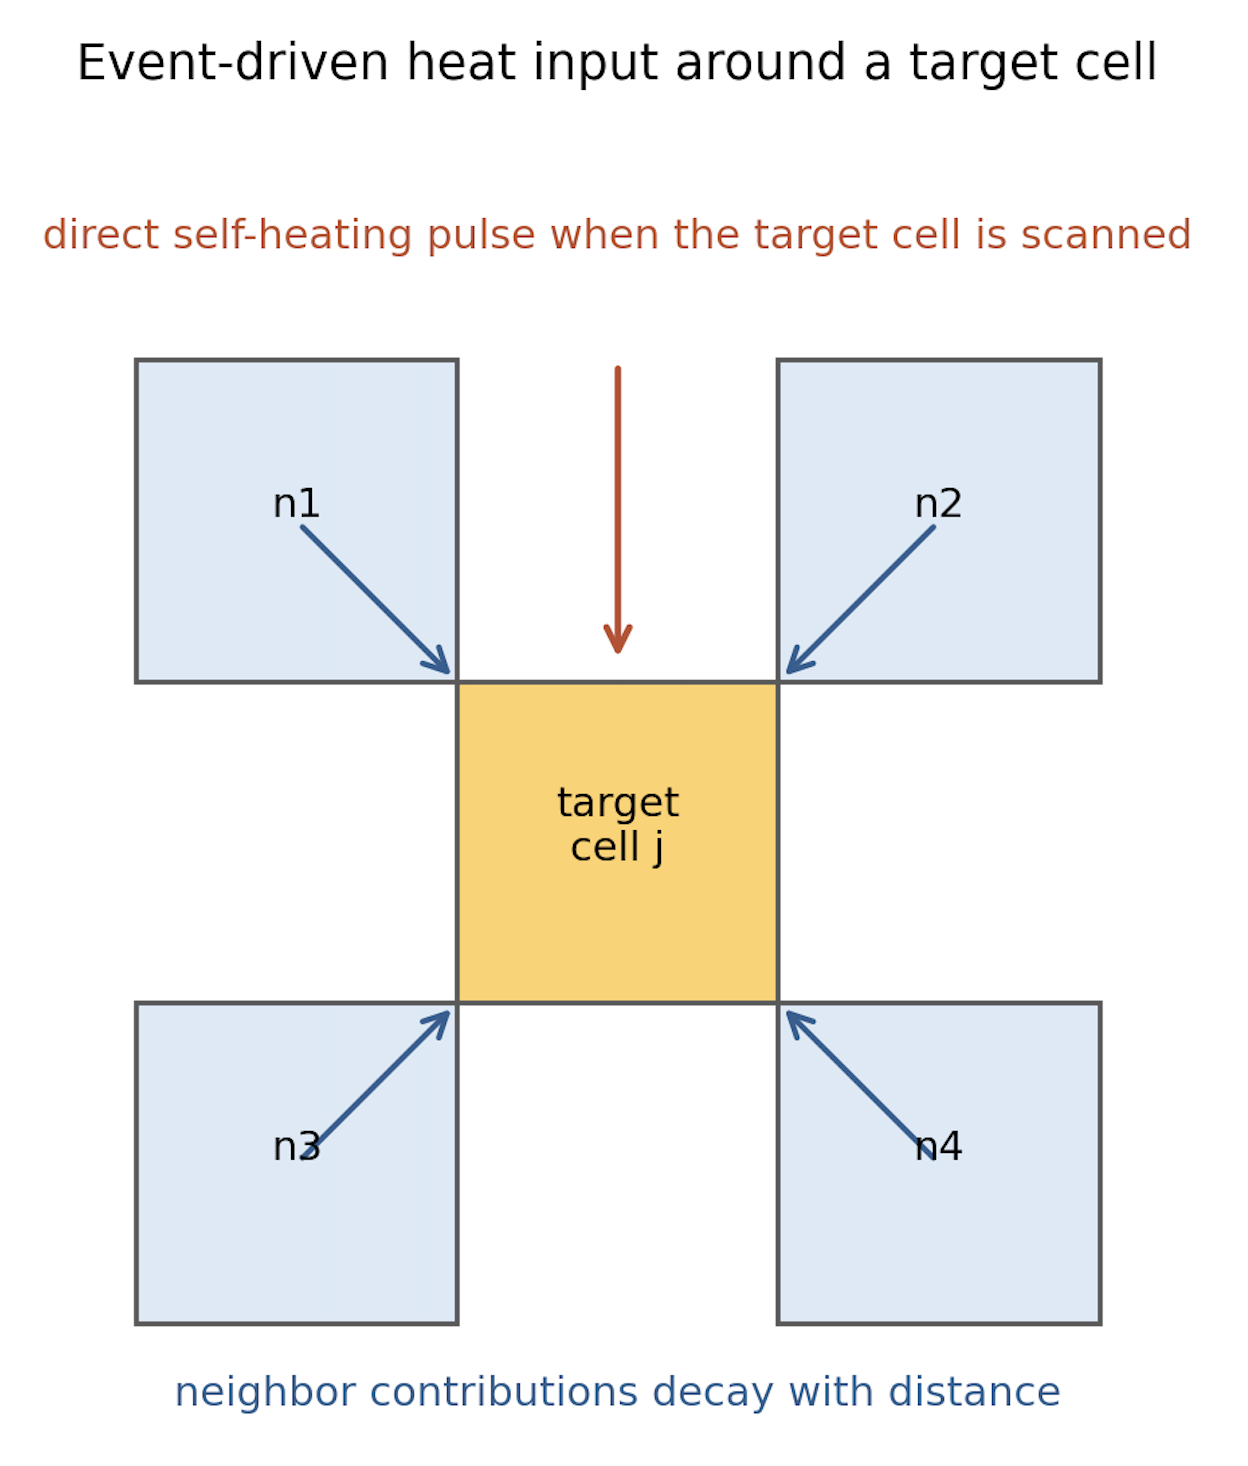
\includegraphics[width=1\linewidth]{截屏2026-04-12 13.44.45.png}
    \caption{热积累机制}
    \label{fig:placeholder}
\end{figure}

\end{minipage}

\hfill
\begin{minipage}[C]{0.5\textwidth}
    \centering
    \vfill
    \textbf{核心思想}：自热 + 历史邻域加热，具有时间衰减和空间衰减。
    \vfill
    
\end{minipage}

\end{comment}


其次，引入接触程度修正项。两个单元之间的热传导效率不仅取决于它们的空间距离，还取决于它们共享边界的长度——共享边界越长，热交换截面越大。定义修正后的接触权重：

\begin{equation}
    w_{ij}^{\text{contact}} = w_{ij}^{\text{spatial}} \left(1 + \gamma \cdot \frac{L_{ij}^{\text{contact}}}{L_0}\right)
\end{equation}

其中 $w_{ij}^{\text{spatial}}$ 为数据文件 \texttt{local\_geometry\_relations.csv} 中提供的空间邻接权重，$L_{ij}^{\text{contact}}$ 为两单元共享边界的长度，$L_0 = 4\,\text{mm}$ 为无量纲化基准长度，$\gamma = 0.5$ 为接触修正系数。该修正使得共边较长的单元对之间的热贡献被适当增强，更符合连续介质热传导的物理图景。

据此，单元 $i$ 对单元 $j$ 在时刻 $t$ 的热贡献表达为：

\begin{equation}
    H_{ij}(t) = q(\pi_j, \pi_i) \cdot \exp\left(-\alpha (t - t_i)\right)
\end{equation}

单元 $j$ 在时刻 $t$ 的累积热积累量为：

\begin{equation}
    H_j^{\text{sum}}(t) = \sum_{i: t_i \le t} H_{ij}(t)
\end{equation}

至此，建立了从扫描时序到单元热积累状态的完整映射关系。

\subsubsection{过热阈值的统计对齐与标定方法}

题目给定原始热贡献模型下的临界阈值 $H_{\text{crit}} = 1.35$，但修正后的热贡献模型改变了热积累量的数值分布形态，直接套用该阈值将失去物理对应性。为此，本文采用分位数对齐法对修正模型下的过热阈值 $H_{\text{thres}}$ 进行统计标定，具体流程如下：

\begin{enumerate}
    \item 选取 \texttt{Row Major} 路径作为固定参考路径——该路径结构规则，可作为不同模型间比较的基准锚点；
    \item 在原始热贡献模型（$A_0 = A_1 = 1$，无质量项，无接触修正）下，计算该路径所有单元的热积累量，获得分布 $\{H_j^{\text{orig}}\}$；
    \item 确定 $H_{\text{crit}} = 1.35$ 在分布 $\{H_j^{\text{orig}}\}$ 中的经验分位数 $q$，即 $q = \frac{1}{N} \sum_{j=1}^{N} \mathbf{1}_{H_j^{\text{orig}} \le H_{\text{crit}}}$；
    \item 在修正后的热贡献模型下，对同一条 \texttt{Row Major} 路径重新计算所有单元的热积累量，获得分布 $\{H_j^{\text{fixed}}\}$；
    \item 取 $\{H_j^{\text{fixed}}\}$ 的第 $q$ 分位数作为修正模型下的过热阈值 $H_{\text{thres}}$。
\end{enumerate}

该方法的本质在于：使修正模型下处于过热状态的单元比例与原始模型保持一致，从而保证 $H_{\text{thres}}$ 与 $H_{\text{crit}}$ 在统计意义上是等价的。在后续灵敏度分析中，每次改变模型参数或材料属性后，均需重复上述标定流程，以确保不同参数组之间的阈值含义一致。


上述对齐逻辑可通过图2直观呈现。如图所示，左右两侧分别展示了原始模型与修正模型下 Row Major 路径的热积累量分布（直方图与累积概率曲线）。其中，选取结构规则、物理一致的 \texttt{Row Major} 路径为基准锚点，分别在原始与修正模型下计算全路径单元的热积累分布。随后，以 $H_{\text{crit}}$ 在原分布中的经验分位数 $q$ 为锚点，对应选取修正分布的 $q$ 分位点作为新阈值 $H_{\text{thres}}$。这一过程确保了“过热单元比例不变”，即无论模型参数如何扰动，阈值的物理含义始终保持统计一致性。每当参数组发生变化，标定流程自动重启，从而保证灵敏度分析具备可比性与物理解释力。

\begin{figure}[H]
    \centering
    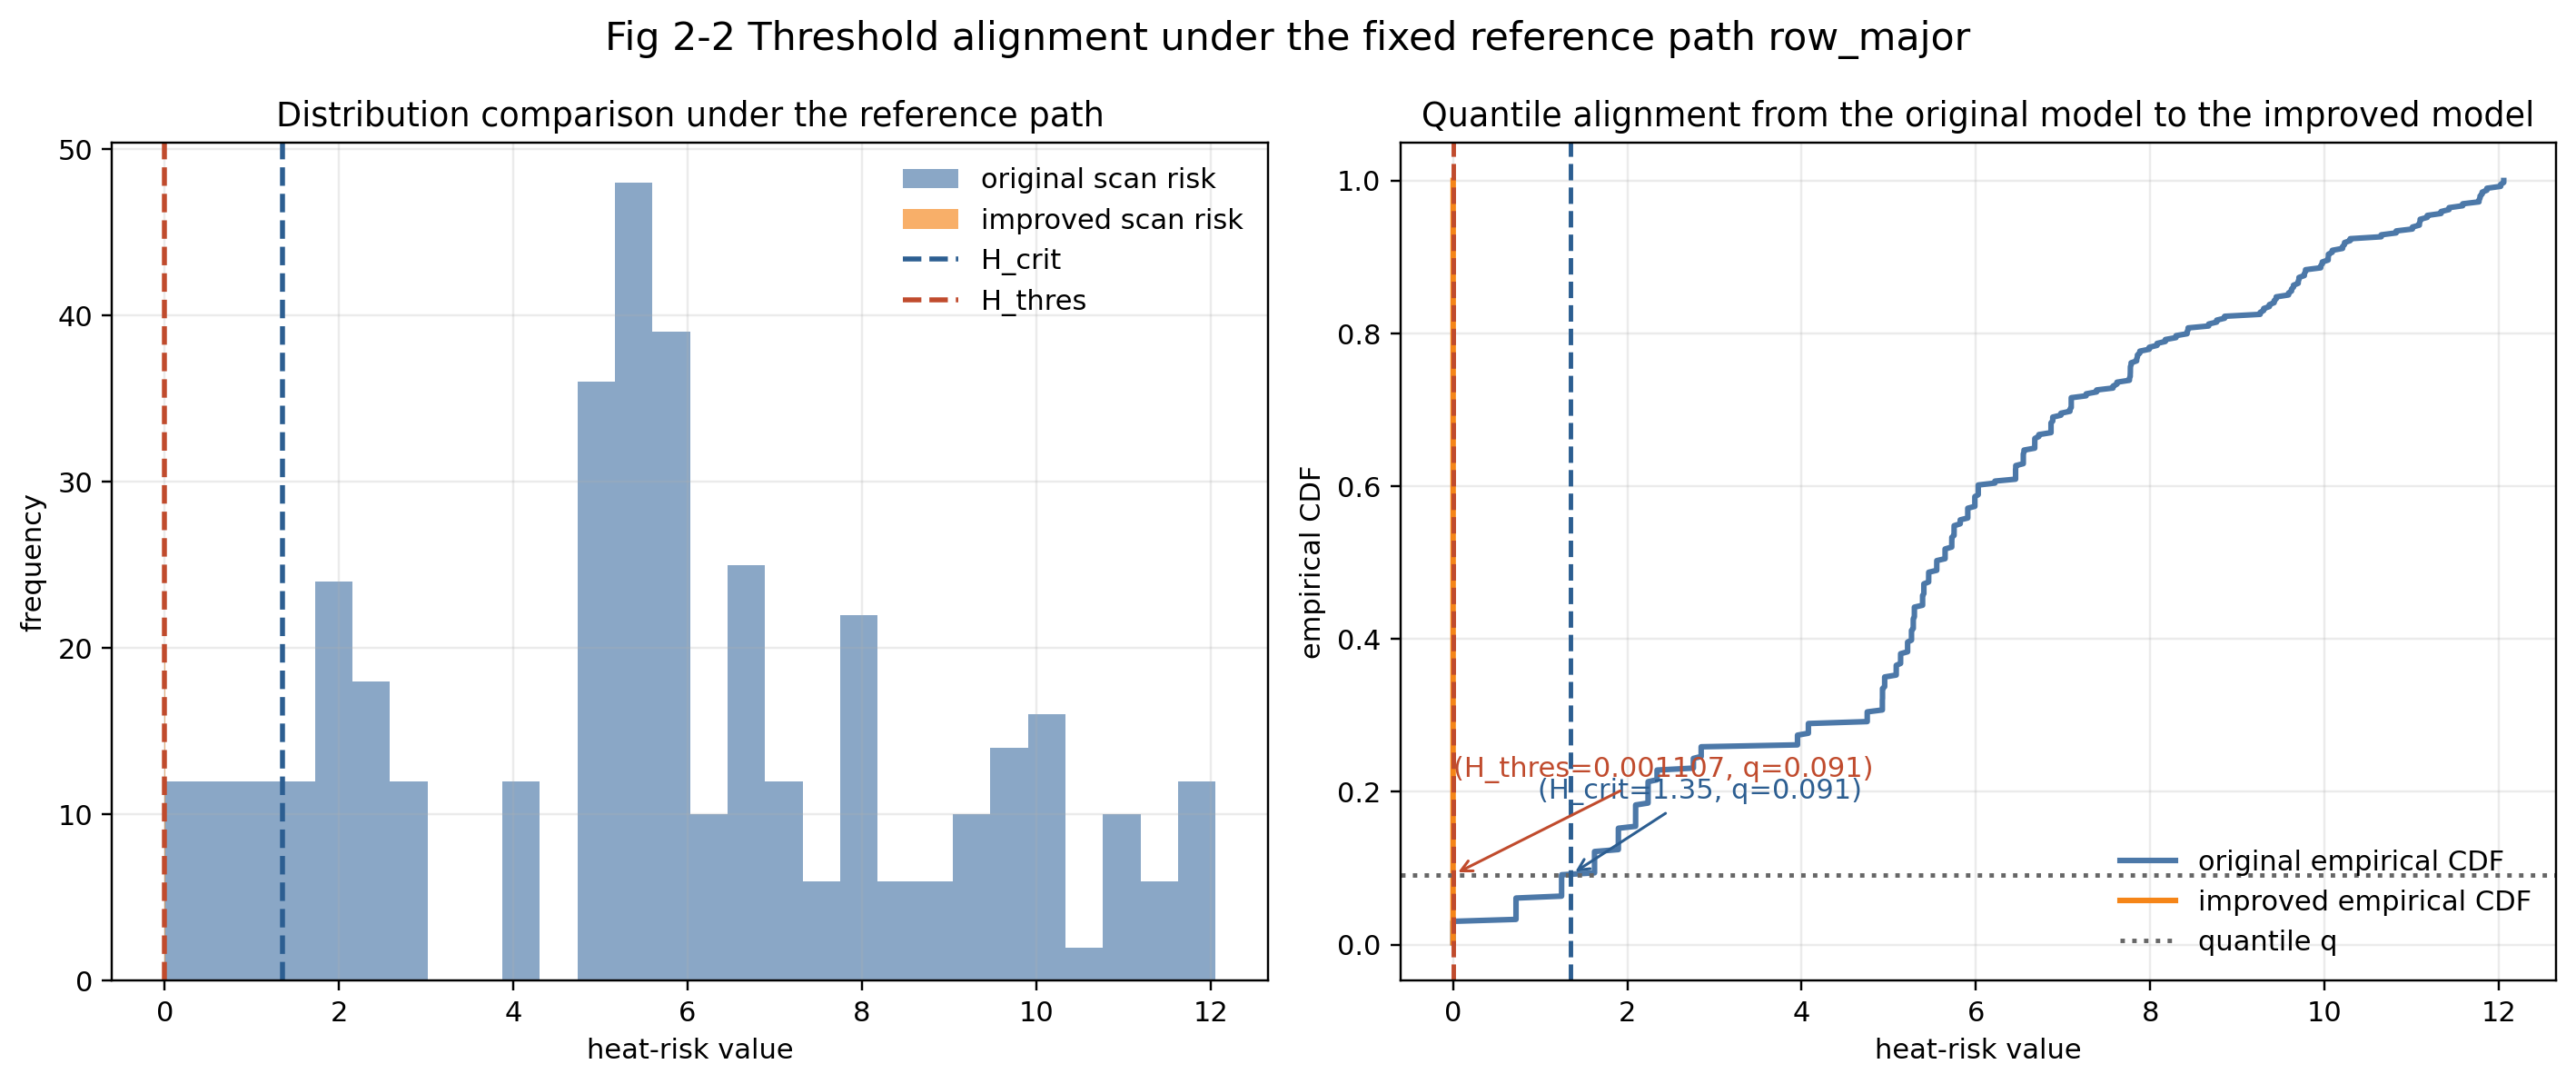
\includegraphics[width=1\linewidth, trim=0 0 0 10mm, clip]{fig2_2_threshold_alignment.png}
    \caption{过热阈值的统计对齐方法}
    \label{fig:placeholder}
\end{figure}



\subsubsection{四类单元级热风险指标的数学定义}

基于前述 $H_j^{\text{sum}}(t)$ 与 $H_{\text{thres}}$，本节给出四个维度风险指标的精确定义。

\textbf{局部高温指数 $\theta_j$}：度量单元 $j$ 在整个扫描过程中累积热积累超过过热阈值的总时间长度。

\begin{equation}
    \theta_j = S_j \cdot \sum_{t = t_{\text{thres}}}^{t_k} \mathbf{1}_{H_j^{\text{sum}}(t) > H_{\text{thres}}}(t)
\end{equation}

其中 $t_{\text{thres}}$ 为单元 $j$ 热积累首次下降至 $H_{\text{thres}}$ 以下的时刻（若从未超过阈值，则 $\theta_j = 0$）；$\mathbf{1}_{(\cdot)}$ 为示性函数；$t_k$ 为层扫描结束时刻。该指标聚焦于“超标”状态的持续时间，反映材料处于危险温度区间的暴露时长。

\textbf{热循环影响指数 $\mu_j$}：度量单元 $j$ 在扫描过程中经历的非自加热升温事件的累积强度。

\begin{equation}
    \mu_j = S_j \cdot \sum_{t = t_j}^{t_k} \mathbf{1}_{\Delta H > 0}(t) \cdot \left[ H_j^{\text{sum}}(t) - H_j^{\text{sum}}(t-1) \right]
\end{equation}

其中 $\mathbf{1}_{\Delta H > 0}(t)$ 指示时刻 $t$ 是否发生了升温事件（相较于前一时刻），求和项累加所有升温阶段的热积累增量。该指标不计入降温阶段的变化量，意在剥离冷却过程的干扰，纯粹表征反复热冲击的累积效应。

\textbf{成型不稳定性指数 $\xi_j$}：度量冷却时间长度对单元 $j$ 成型的影响。

\begin{equation}
    \xi_j = S_j \cdot (t_{H^{sum}_j(t) < H_{thres}} - t_j)
\end{equation}

其中 $t_{H^{sum}_j(t) < H_{thres}}$ 为单元 $j$ 在扫描完成后完全冷却（热积累低于阈值 $H_{thres}$ ）的时刻。该指标用于表征材料成型稳定性，冷却时间越长、材料本身的热鲁棒性越差，材料越可能在成型的过程中发生形变。

\textbf{邻域热分布不均匀性指数 $\phi_j$}：度量单元 $j$ 与其相邻单元之间在整个扫描过程中的平均热积累差异。

\begin{equation}
    \phi_j = \frac{1}{k} \sum_{n=1}^{k} \frac{ \sum_{\pi_i \in E_j} w_{ij}^{\text{contact}} \left| H_j^{\text{sum}}(t_n) - H_i^{\text{sum}}(t_n) \right| }{ \sum_{\pi_i \in E_j} w_{ij}^{\text{contact}} }
\end{equation}

其中 $E_j$ 为与单元 $j$ 有公共边的邻接单元集合，$w_{ij}^{\text{contact}}$ 为前述接触权重，$k$ 为当前层单元总数，$t_n$ 为第 $n$ 个扫描事件发生的时刻。该指标在每一个扫描事件时刻均计算一次邻域温差，然后取全过程的平均值，反映的是热分布均匀性的整体水平而非瞬时状态。

\subsubsection{从单元指标到路径方案的综合评价}

计算得到所有单元的四类指标后，需进一步聚合为可比较的路径级综合得分。本文采用双层综合评价架构：底层使用熵权法确定每类指标内部特征维度的权重，上层采用加权和法融合四类指标。

对于每类指标，提取若干统计特征以刻画其分布形态。以热循环影响指数 $\mu$ 为例，选取均值 $\bar{\mu}$ 与头部10\%均值 $\bar{\mu}_{10\%}$。头部均值的引入旨在捕捉极端高风险单元的贡献，避免单纯使用均值时极端值被淹没。各指标的特征选取如下：

\begin{table}[H]
    \centering
    \caption{单元级风险指标的特征选取与统计量定义}
    \label{tab:risk_features}
    \begin{tabular}{cccc}
        \toprule
        指标 & 符号 & 选取的统计特征 \\
        \midrule
        局部高温指数 & $\theta$ & 均值 $\bar{\theta}$、头部10\%均值 $\bar{\theta}_{10\%}$  \\
        热循环影响指数 & $\mu$ & 均值 $\bar{\mu}$、头部10\%均值 $\bar{\mu}_{10\%}$  \\
        成型不稳定性指数 & $\xi$ & 均值 $\bar{\xi}$、极大值 $\xi_{\max}$  \\
        邻域热分布不均匀性指数 & $\phi$ & 均值 $\bar{\phi}$、头部10\%均值 $\bar{\phi}_{10\%}$、极大值 $\phi_{\max}$  \\
        \bottomrule
    \end{tabular}
\end{table}

采用熵权法确定每个指标内部各特征的权重。熵权法的基本原理是：数据变异程度越大的特征，其所蕴含的信息量越丰富，应赋予更高的权重。该方法避免了人为指定权重的主观性，使评价结果更具客观性。记特征 $f$ 的熵值为 $e_f$，则其权重为：

\begin{equation}
    \omega_f = \frac{1 - e_f}{\sum_{f'} (1 - e_{f'})}
\end{equation}

据此，四类指标的二级得分计算如下：

\begin{equation}
    R_{\theta} = \omega_{\bar{\theta}} \bar{\theta} + \omega_{\bar{\theta}_{10\%}} \bar{\theta}_{10\%}
\end{equation}
\begin{equation}
    R_{\mu} = \omega_{\bar{\mu}} \bar{\mu} + \omega_{\bar{\mu}_{10\%}} \bar{\mu}_{10\%}
\end{equation}
\begin{equation}
    R_{\xi} = \omega_{\bar{\xi}} \bar{\xi} + \omega_{\xi_{\max}} \xi_{\max}
\end{equation}
\begin{equation}
    R_{\phi} = \omega_{\bar{\phi}} \bar{\phi} + \omega_{\bar{\phi}_{10\%}} \bar{\phi}_{10\%} + \omega_{\phi_{\max}} \phi_{\max}
\end{equation}

最后，通过加权和法计算路径的综合热风险得分：

\begin{equation}
    R_{\text{total}} = \omega_{\theta} R_{\theta} + \omega_{\mu} R_{\mu} + \omega_{\xi} R_{\xi} + \omega_{\phi} R_{\phi}
\end{equation}

一级权重 $(\omega_{\theta}, \omega_{\mu}, \omega_{\xi}, \omega_{\phi})$ 反映建模者对四个风险维度重要性的先验判断。本文在基础模型中设定为 $(0.35, 0.20, 0.20, 0.25)$，其中局部高温权重最高，因其对成形质量的直接危害最为显著；邻域温差次之，因其与翘曲变形的关联紧密。该组权重的主观性将在后续灵敏度分析中进行系统检验。



\vspace{1em}
\section{算法性能验证与基准方案多维对比}
\vspace{0.5em}

为验证本文构建的全局时间最优路径寻优模型在复杂几何边界与典型工业约束下的性能边界，本节引入三种工业界广泛采用的基准扫描策略，从宏观多维效能指标与微观拓扑几何特征两个维度开展对等横向评价。

\subsection{典型工业基准扫描策略与对比环境设定}

本文提取了赛题数据及实际 LPBF 生产中的三种典型工业基准方案：
\begin{itemize}
    \item \textbf{顺序扫描 (Row Major)}：遵循严格的网格行列递增遍历逻辑。该策略空间复杂度极低，但在面临非连通域或复杂拓扑边界时，极易诱发高频的冗余空走跳跃。
    \item \textbf{蛇形扫描 (Serpentine)}：采用“S”型连续折返扫描矢量覆盖加工域。该方法可有效抑制行间跳转频率，但其路径刚性较强，对异形边界的自适应性不足。
    \item \textbf{中心向外扫描 (Center Out)}：由几何中心呈辐射状向外缘延展。该策略在热力学层面利于中心热量耗散，但在受限几何边界下的寻迹效率表现往往欠佳。
\end{itemize}

\subsection{问题一：时间最优路径的降本增效验证}

针对第一问构建的全局时间最优路径规划模型，本节旨在通过与三种典型工业基准策略的对等基准测试，全面验证其在 LPBP 工艺中的“降本增效”潜能。本节的论证逻辑遵循“宏观效能统揽，微观机理溯源”的分析框架：首先从全局时空域提取空走距离与时间特征进行定量横向评价；随后深入单层复杂非连通域的几何边界，剖析本算法在寻迹拓扑上的自适应机理，从而为路径的高效性提供严密的数据与几何双重支撑。

\subsubsection{宏观效能：全局空走规避与时域极限压缩}
将本文求解得到的 Optimal 与上述三种基准策略进行对比，提取Part A 所有层聚合情况下的总空走距离与层内总时间，其宏观效能表现如图 \ref{fig:performance_comparison} 所示。

\begin{figure}
    \centering
    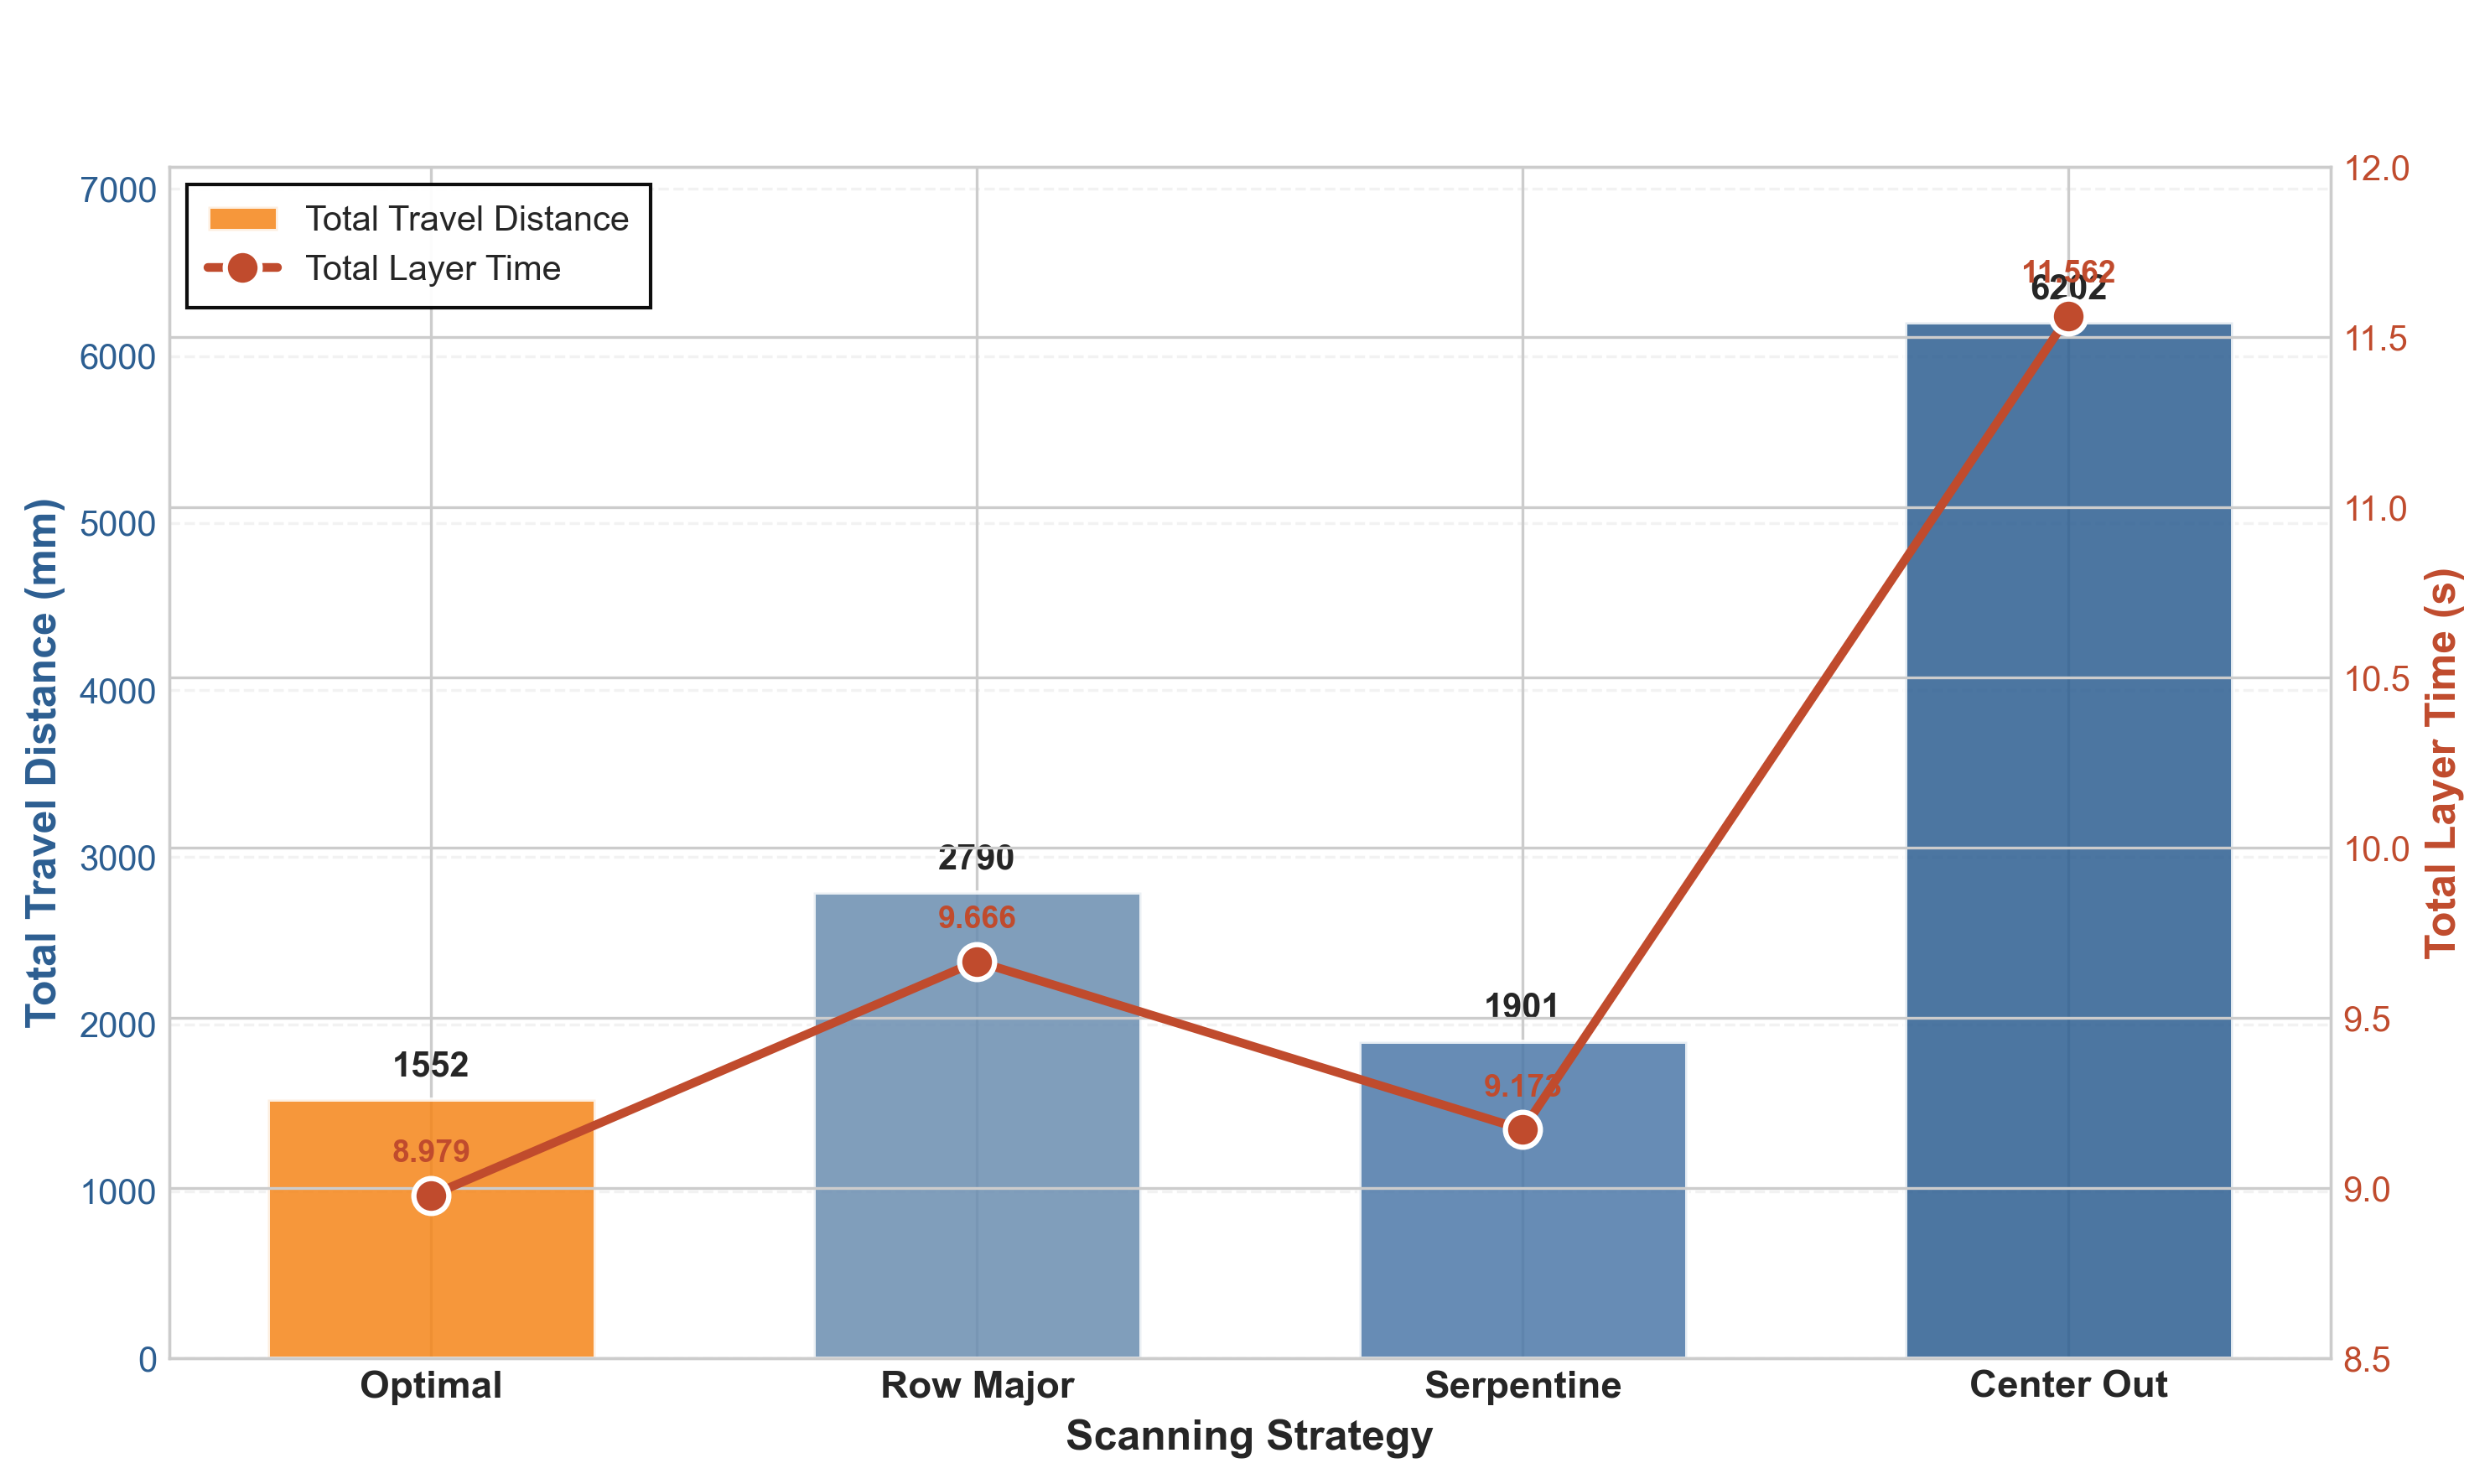
\includegraphics[width=0.85\linewidth]{performance_comparison.png}
    \caption{Part A 全层级多策略空走距离与层内总时间对比双轴图}
    \label{fig:placeholder}
\end{figure}

分析图 \ref{fig:performance_comparison} 的双维特征分布可知，本文寻优模型在空走距离的控制上展现出极优异的收敛性。其全层累计空走距离被压缩至 $1552\text{ mm}$，相较于工业标准 Row Major 策略（$2789.7\text{ mm}$）实现了约 $44.4\%$ 的距离削减；反观 Center Out 策略，因受强制中心发散逻辑引发的冗余跳转影响，其空走距离高达 $6201.7\text{ mm}$，效能最劣。

在核心标量目标“层内总时间”维度，本文模型同样录得全局极小值（$8.979\text{ s}$）。值得强调的是，鉴于粉末床熔融工艺中“有效曝光时间”系由零件截面物理面积严格锚定的常数，算法的优化可行域仅局限于“空走耗时”与“跳转启停延迟”。在此时域强约束条件下，本文算法依然实现了单层绝对耗时的有效压缩，有力论证了其逼近全局理论下界的寻优效能。

\subsubsection{微观几何：非连通域边界下的拓扑自适应}

为探究上述宏观时间效能增益的底层空间机制，本文以 Part A 几何拓扑最为复杂的第 3 层为例（具备典型的多连通域特征与内孔避让约束），重构并提取了四类策略的微观路径拓扑映射（如图 \ref{fig:path_topology} 所示）。

\begin{figure}[H]
    \centering
    % 请确保图片命名与你的实际生成文件一致
    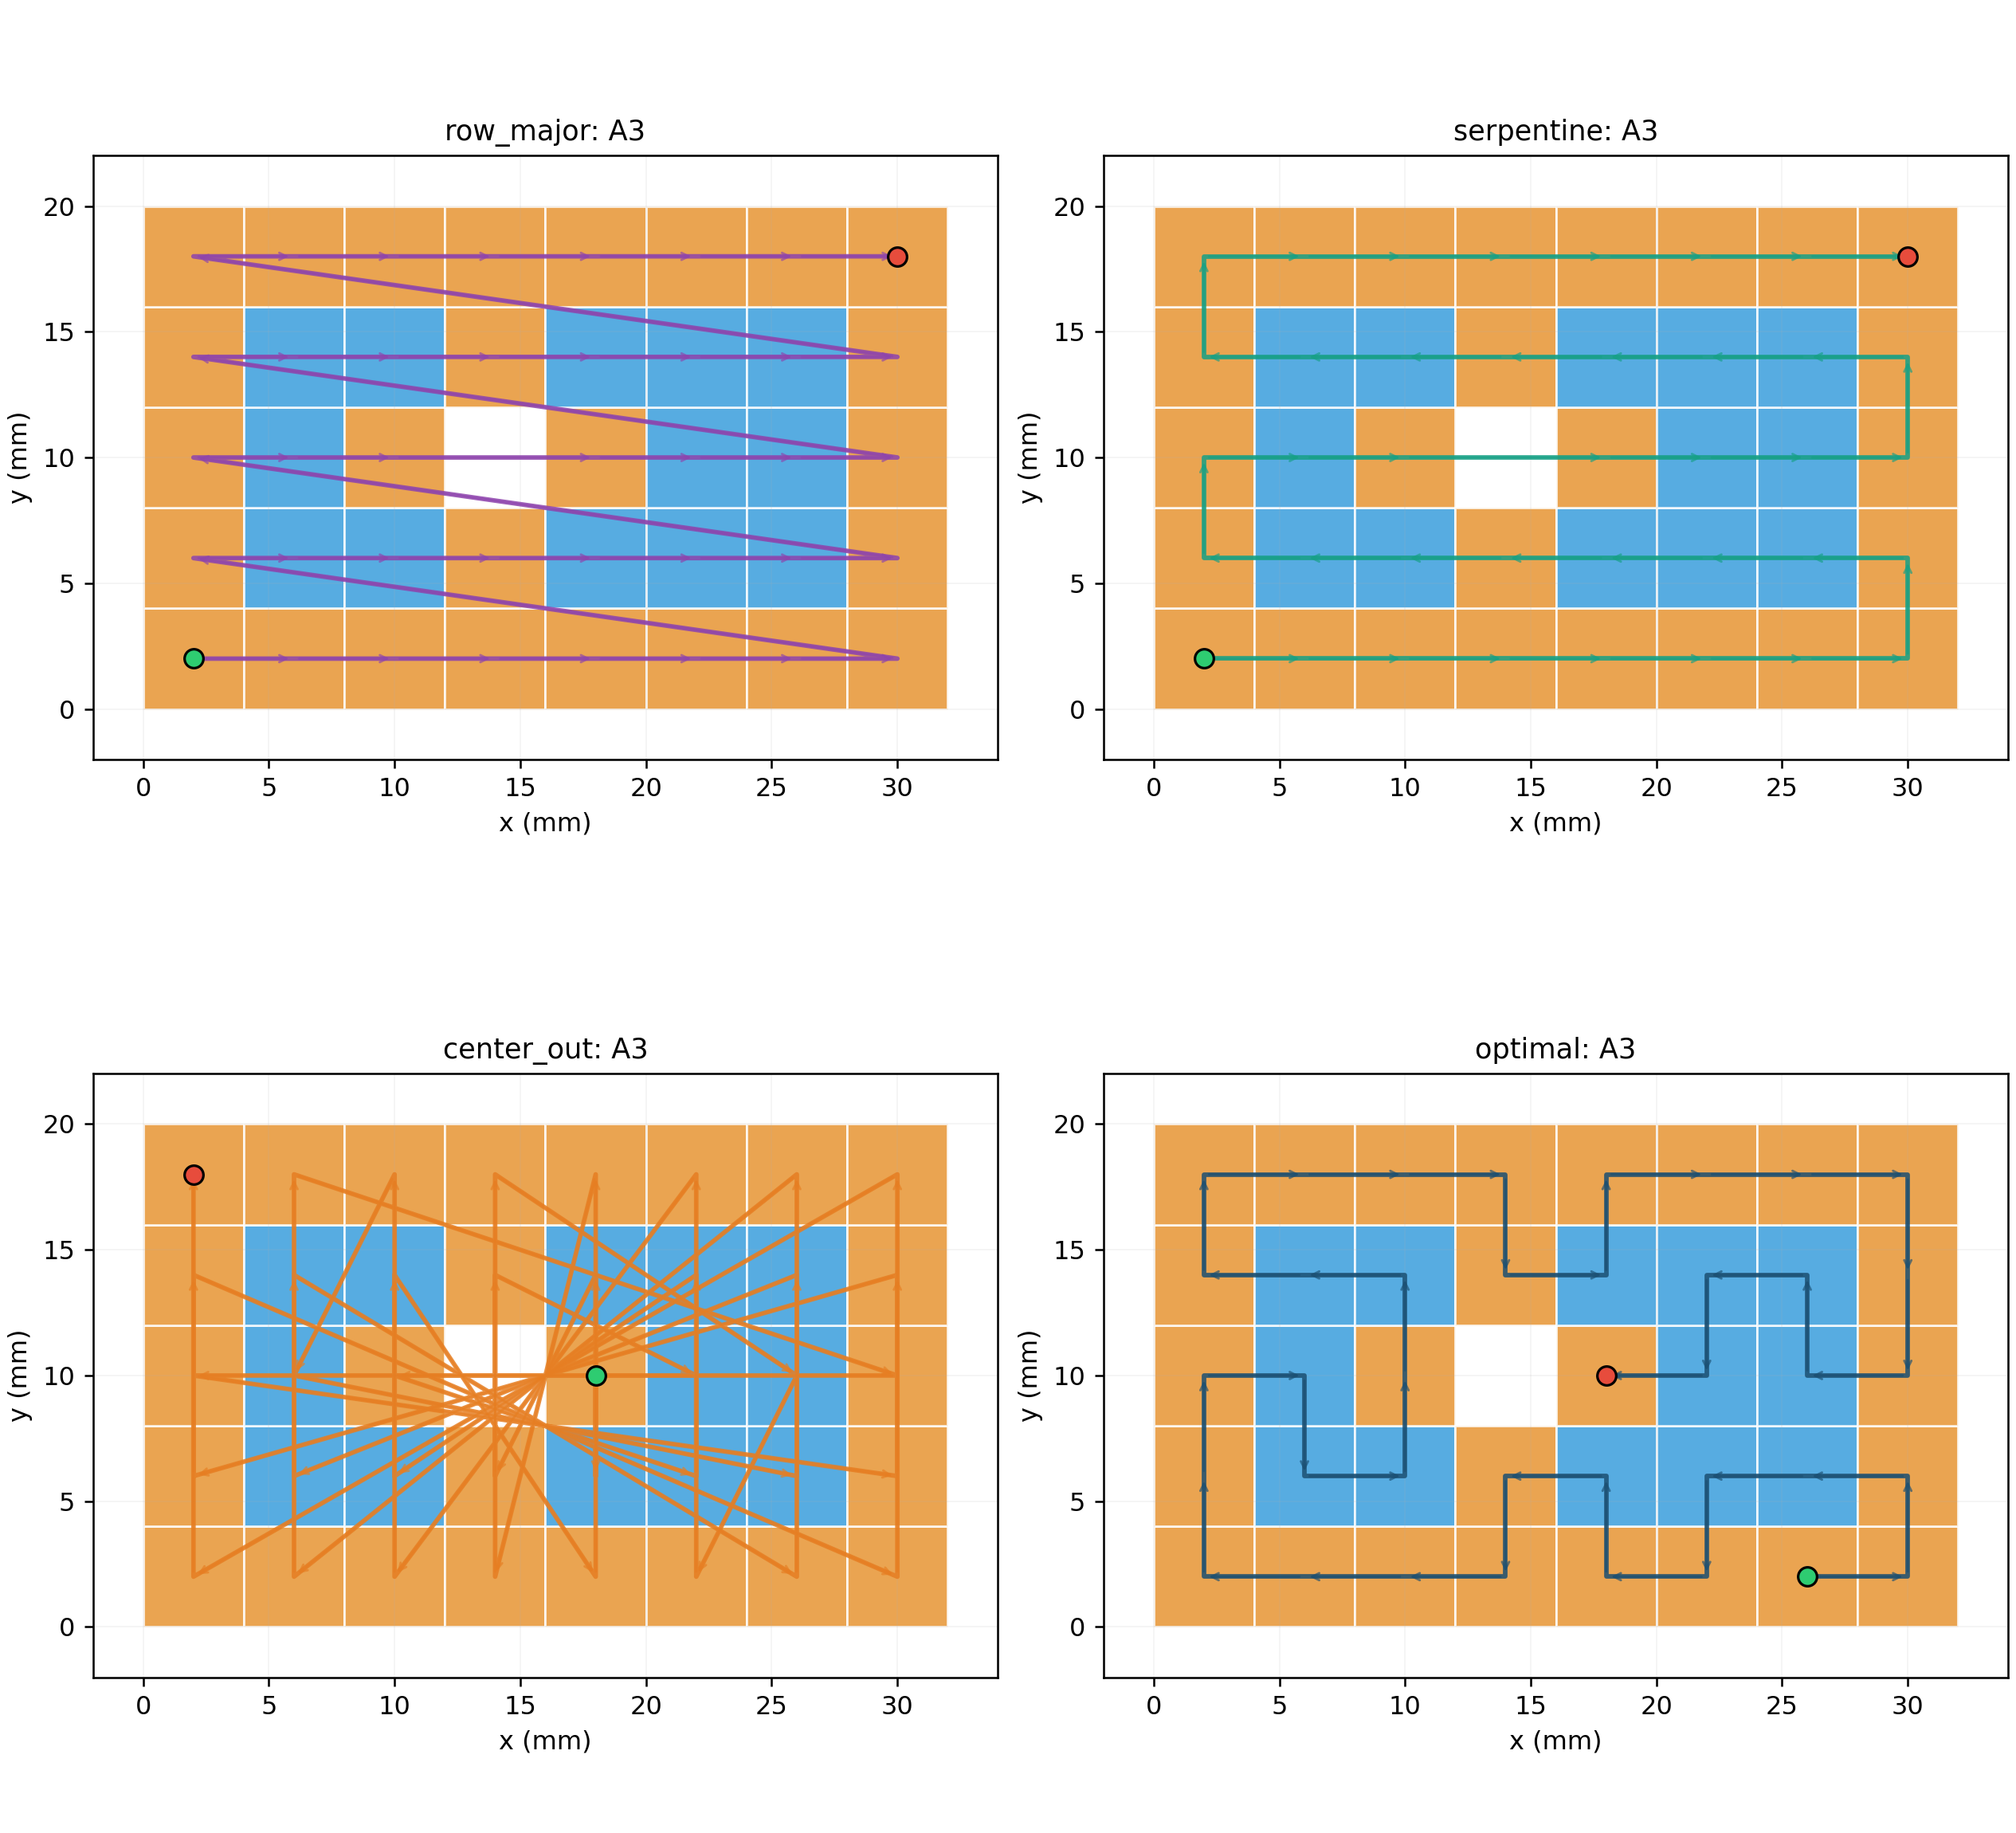
\includegraphics[width=1.0\textwidth, trim=0 0 0 10mm, clip]{baseline_vs_optimal_path_part_A.png}
    \caption{不同扫描策略在复杂多连通域边界下的微观路径拓扑对比 (Part A 第 3 层)}
    \label{fig:path_topology}
\end{figure}

观察图 \ref{fig:path_topology} 的微观寻迹轨迹可进一步印证前文的数据结论：
基准方案 Row Major 与 Serpentine 虽呈现出高度的各向异性规则排列，但受限于固化的扫描范式，在面临非扫描域（中间孔洞）的阻断时，不可避免地激发了高频且长距离的跨区跃迁（直观表现为贯穿式连线）。Center Out 策略则受制于中心辐射约束，导致了极其密集的无序长程空走，极大劣化了加工节拍。

与此形成显著对比，本文 Optimal 路径展现出优异的“局部空间聚类”与“就近遍历”特征。该路径不仅在子连通域内实现了连续紧凑覆盖，且在跨域过渡阶段实现了基于最短欧氏距离的平滑接力，从根源上规避了冗余的空间震荡。此种对复杂异形边界的高鲁棒性自适应机制，构成了本文算法显著降低全局空走距离与成型时间的数理本质。

\subsection{问题二：多维热力学风险的安全评估验证}

将前述综合评价框架应用于四条候选扫描路径：Row Major、Serpentine、Center Out 以及第一问求解得到的时间最优路径。为深究不同空间布线策略对热场演化的干预机制，本文首先从微观单元视角提取了热状态的空间拓扑与统计分布。

\begin{figure}[H]
    \centering
    % 请放置 fig2_3_final_heat_map.png
    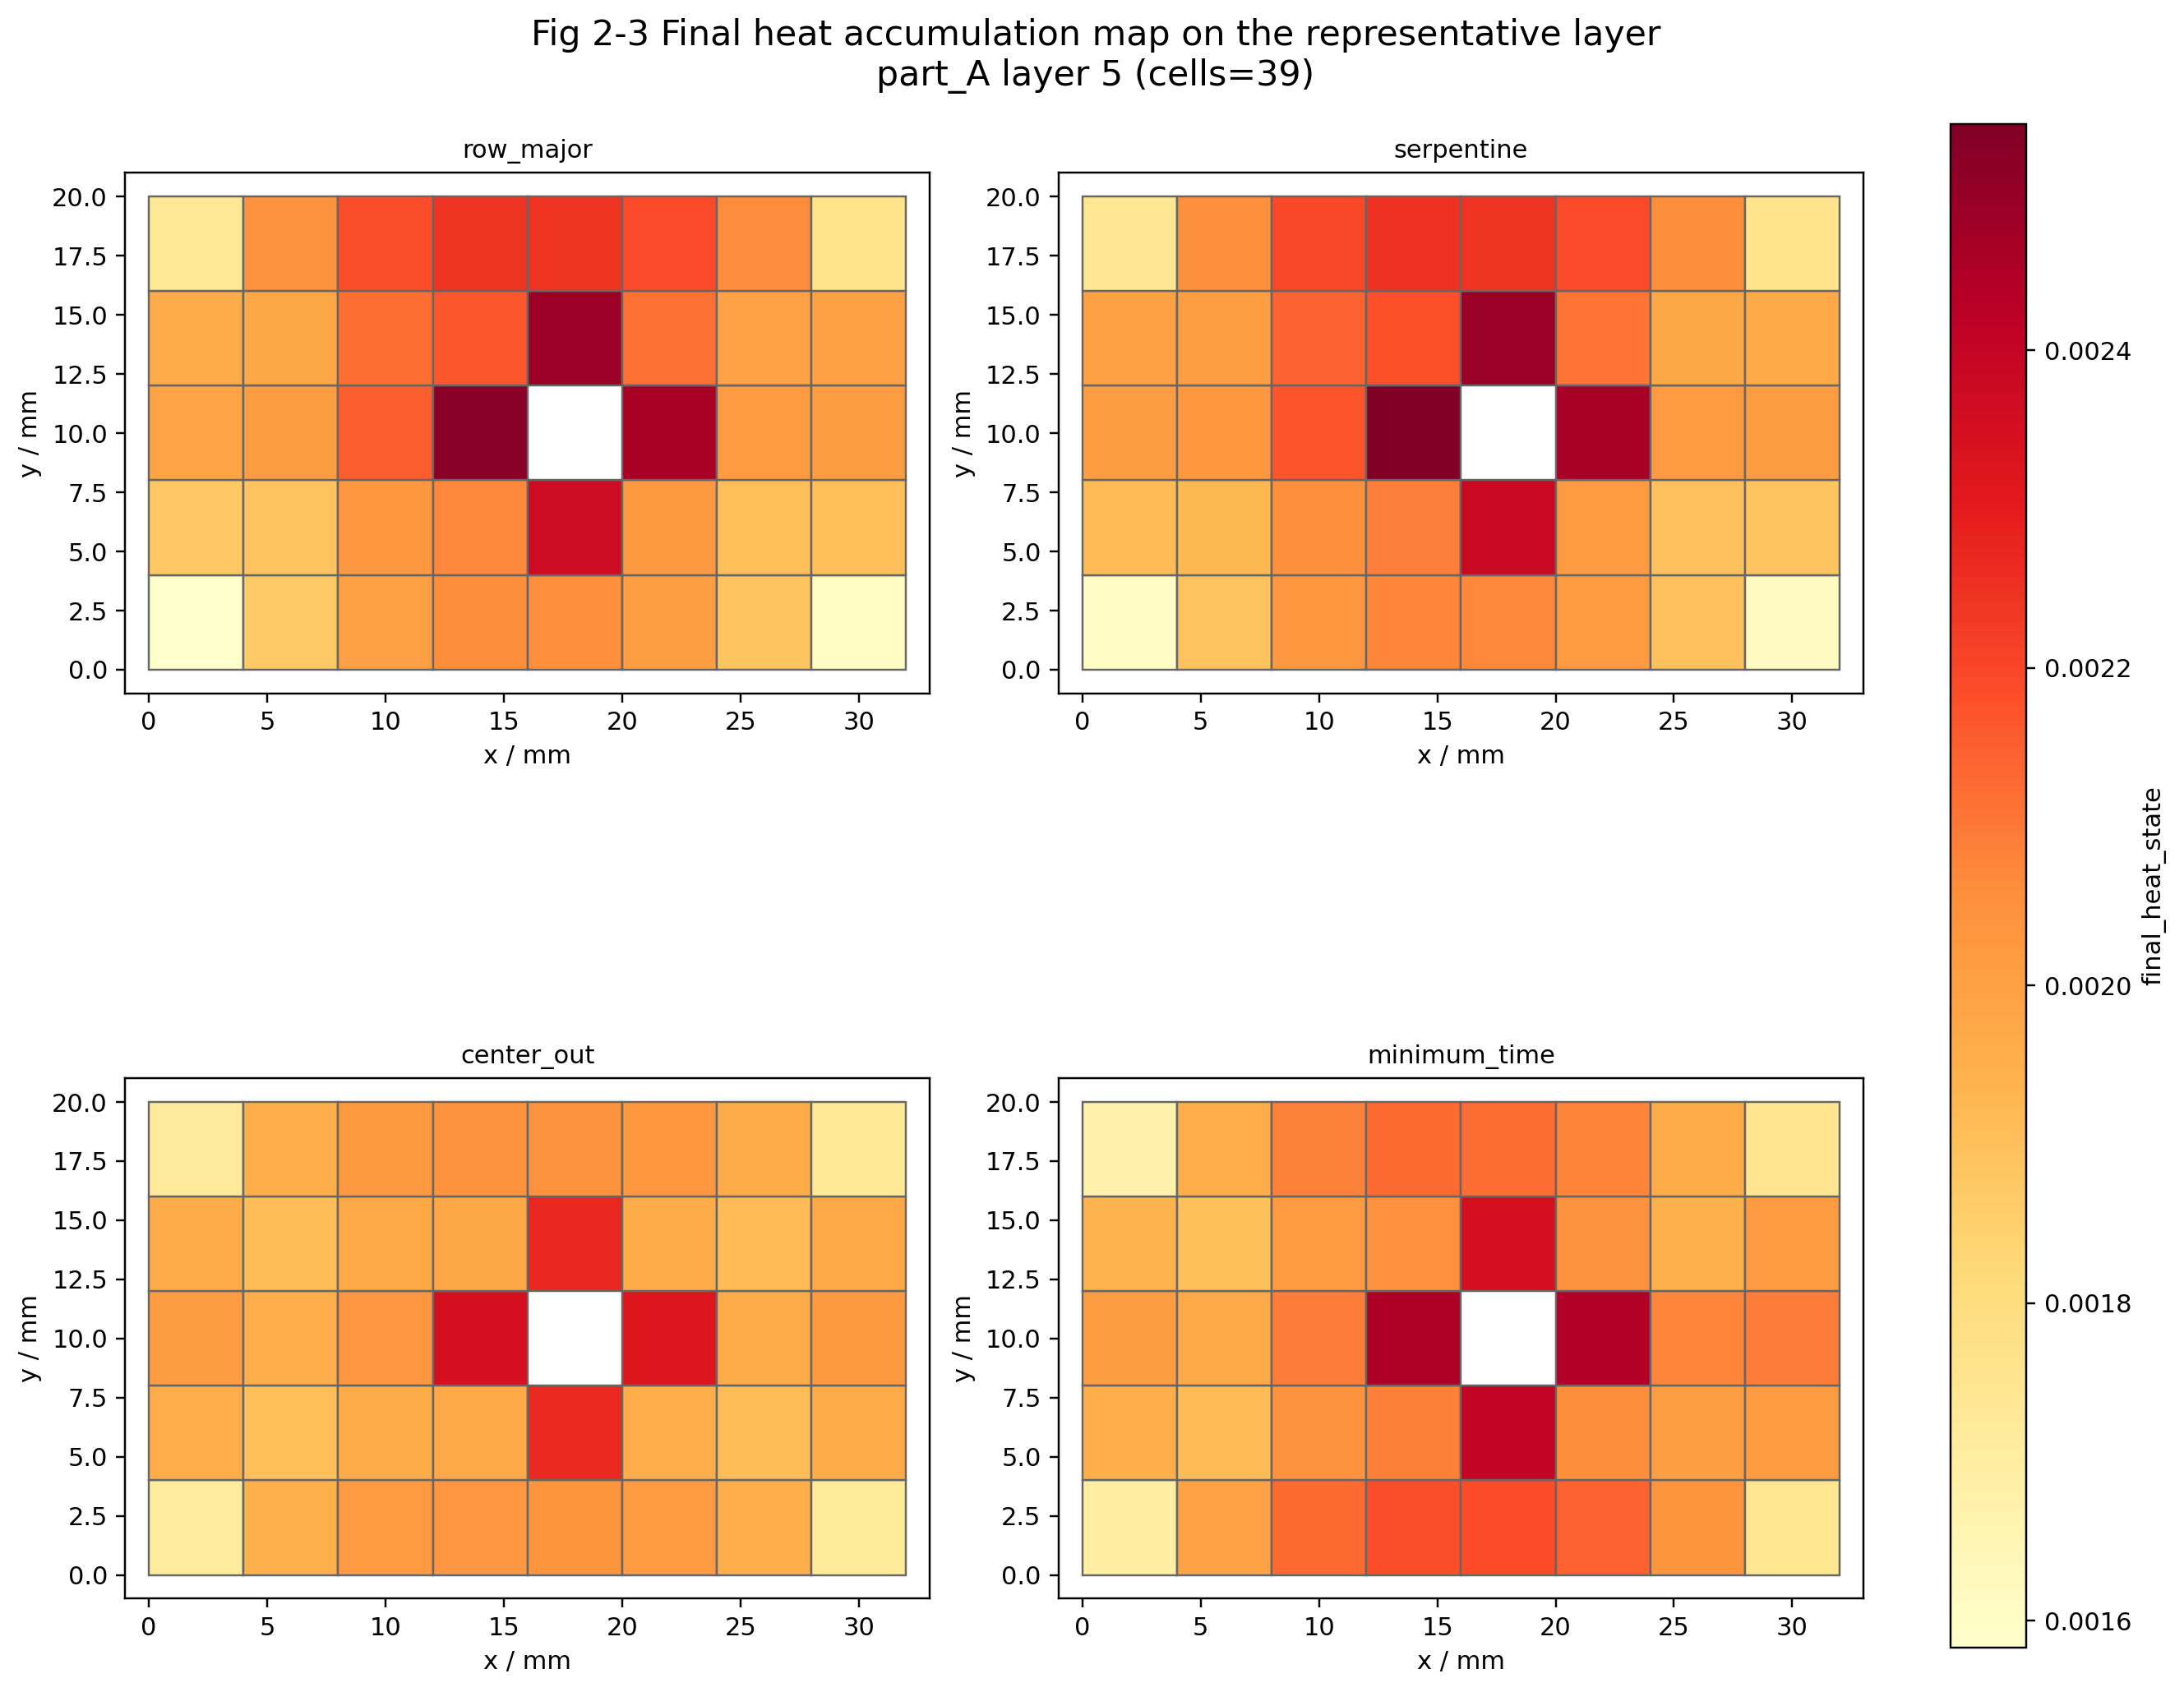
\includegraphics[width=0.9\textwidth, trim=0 0 0 20mm, clip]{fig2_3_final_heat_map.png}
    \caption{不同扫描策略在代表层（Part A 第 5 层）的最终热积累空间分布映射}
    \label{fig:final_heat_map}
\end{figure}

图 \ref{fig:final_heat_map} 展示了代表层加工结束时的最终热积累映射。受限于几何边界，各策略的热点（暗红色区域）不可避免地向中心孔洞等散热受限的狭窄相交区域富集。然而，不同路径对热场的微观调控能力存在显著差异。

\begin{figure}[H]
    \centering
    % 请放置 fig2_13_cell_risk_boxplots.png
    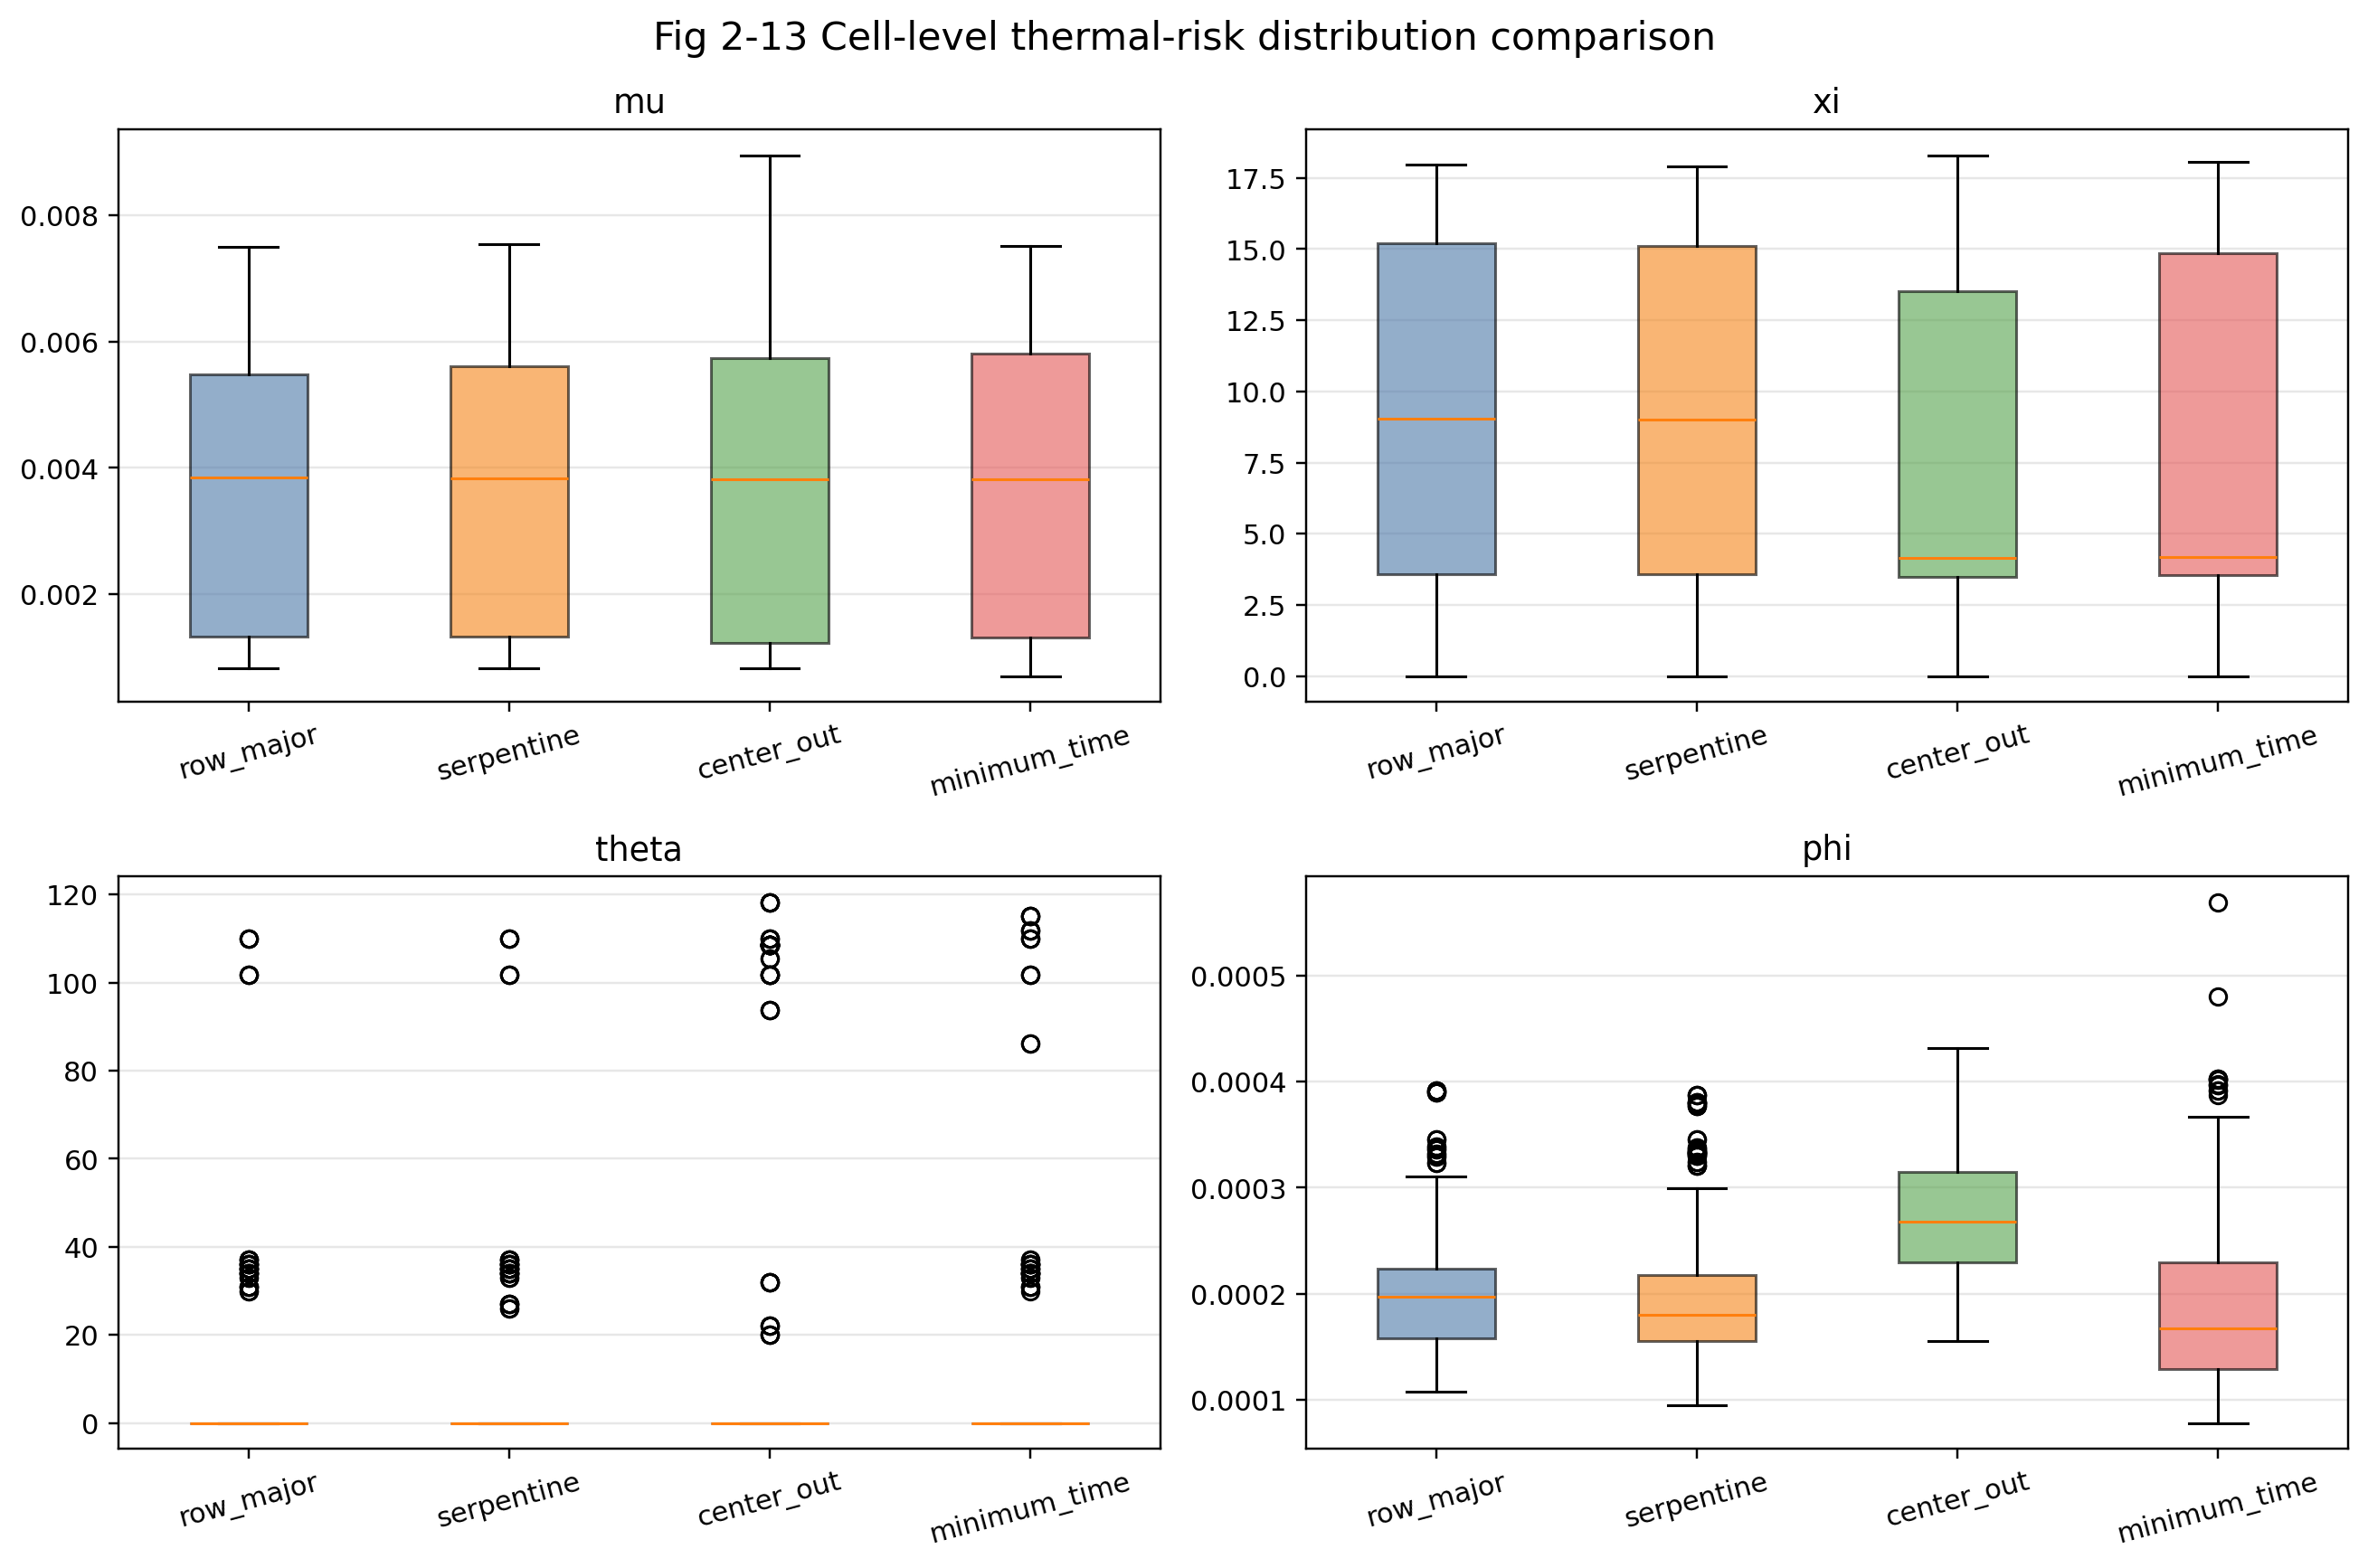
\includegraphics[width=0.9\textwidth, trim=0 0 0 10mm, clip]{fig2_13_cell_risk_boxplots.png}
    \caption{不同扫描策略下单元级多维热风险指标的离散程度与箱线图统计}
    \label{fig:cell_risk_boxplots}
\end{figure}

进一步提取全任务的单元风险指标统计特性（见图 \ref{fig:cell_risk_boxplots}），深刻揭示了不同布线策略在微观热场调控上的差异化物理演化机制：

\begin{itemize}
    \item \textbf{时间最优路径的局部热高峰聚积（热过载现象）}：第一问求解的时间最优路径虽在邻域热均匀性 $\phi$ 上表现优异（中位数处于极低水平），但其在局部高温指数 $\theta$ 上诱发了大量极其危险的超高异常值（极大值突破 110）。其内在物理机制在于：该算法为追求极致的空走距离压缩，驱使热源在局部微小连通域内进行高频连续曝光，导致局部热量在极短的冷却窗口内急剧恶化。
    
    \item \textbf{分层平行策略的天然热量缓冲效应}：相比之下，Row Major 与 Serpentine 策略虽然牺牲了少量空走时间，但其规则的长程交替行进特征充当了天然的“热量缓冲带”。这种更为充裕的空间位移极其有效地抑制了极端高温事件与剧烈热循环冲击的爆发，展现出极高的热稳健性。
    
    \item \textbf{辐射扩展策略的全局热失控陷阱}：Center Out 策略受制于中心辐射所引发的空间错乱与长程跳转，其在所有热危险指标上的方差离散度与极端异常值均表现最劣，呈现出极不稳定的系统热态。
\end{itemize}

\subsection{一二问统筹：基于帕累托前沿的产能与质量联合权衡}

在真实的增材制造工程实践中，打印时间（表征产能）与热积累量级（表征成型质量）往往构成一对相互拮抗的博弈目标。为客观评估各方案的工程落地价值，本文将单层平均加工时间与加权热风险总分映射至双维决策空间（见图 \ref{fig:pareto_time_risk}）。

\begin{figure}[H]
    \centering
    % 请放置 fig2_14_pareto_time_risk.png
    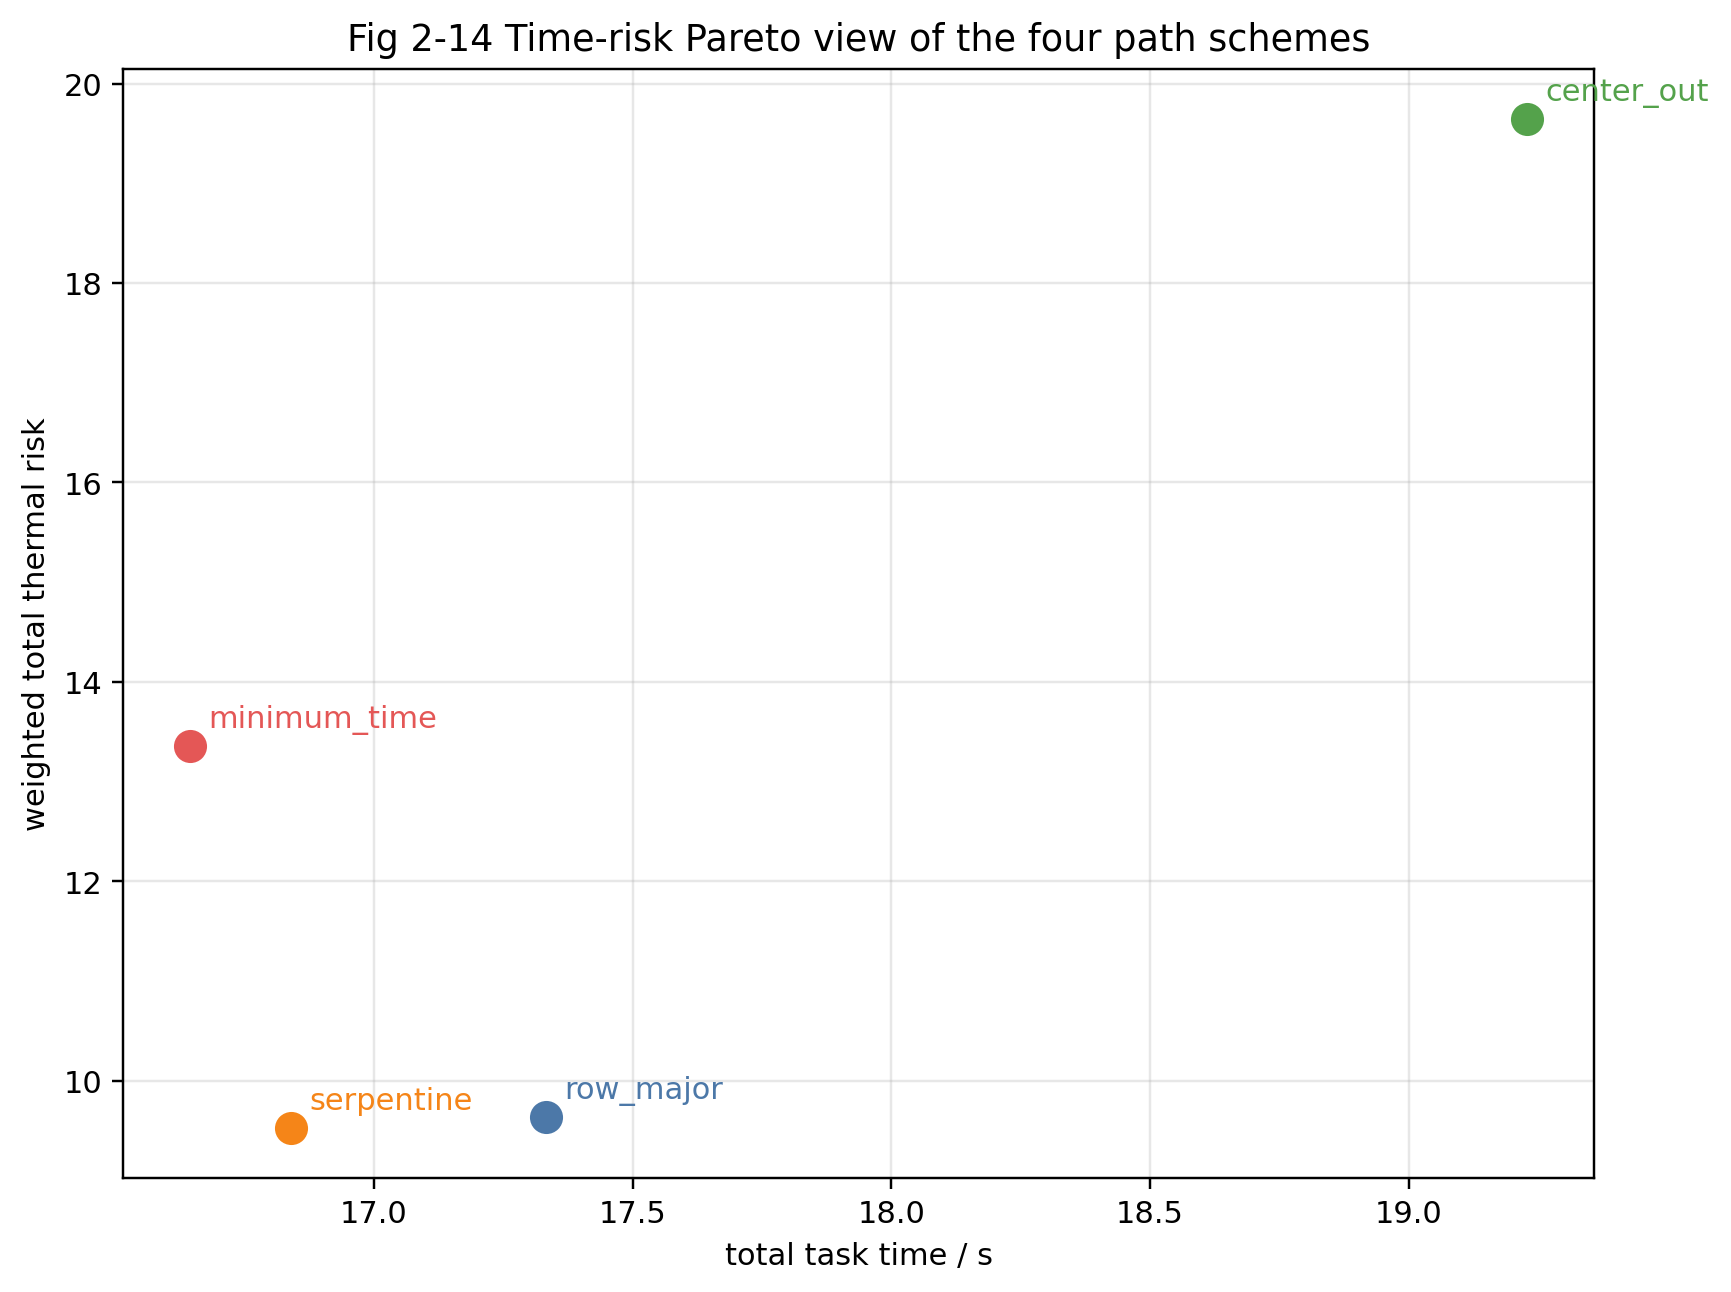
\includegraphics[width=0.75\textwidth, trim=0 0 0 7.8mm, clip]{fig2_14_pareto_time_risk.png}
    \caption{四类扫描策略在时间效率与综合热风险维度的帕累托散点评价}
    \label{fig:pareto_time_risk}
\end{figure}

散点拓扑分布清晰地界定了各方案的效能边界：
Center Out 方案处于决策空间的最劣象限（高耗时、高风险），属于典型的受支配解，在工业生产中应予严格规避。其余三条路径则共同构筑了该系统的帕累托前沿：
第一问求解的最优时间路径牢牢占据了前沿最左端，取得了绝对的时间霸权，但在综合热风险上相较于最优基准线付出了约 $38\%$ 的质量惩罚。而 Row Major 与 Serpentine 方案则占据了前沿底部，构筑了热安全性能的理论下界。

这一多维对比结论极具启发性：空间距离的极小化并不等价于热力学状态的全局最优。第一问求得的连续扫描轨迹并未打破传热物理定律的客观制约，而是用局部的“时间密度”透支了“热耗散窗口”。因此，在实际 LPBF 工艺决策中，若追求极致产能且材料热鲁棒性较好，首选时间最优路径；若打印钛合金等易残余应力开裂的高热敏感材料，则应坚定选用 Serpentine 等平行类路径。



\vspace{1em}
\section{灵敏度分析}
\vspace{0.5em}

\subsection{问题一：时间模型的灵敏度分析}
为了考察模型结论的稳健性，本节从结果灵敏度和解结构灵敏度两个层面进行分析。

\subsubsection{结果灵敏度分析}

在增材制造的实际物理加工过程中，设备的运动学参数（如空走速度、激光开启延迟等）往往会因硬件性能限制或工艺设定偏差而发生波动。为验证本模型在多变物理环境下的时间成本稳定性，本节针对核心速度参数展开定量的灵敏度分析。

\vspace{0.5em}
\noindent\textbf{（1）空走速度扰动下的多策略优越性与稳定性分析}
\vspace{0.5em}

为精确量化空走速度变化对模型稳定性的影响，我们将本文算法（Optimal）与三种工业基准策略（Row Major, Serpentine, Center Out）进行了横向对比。图 \ref{fig:jump_speed_heatmap} 展示了在 1200 mm/s 至 2400 mm/s 速度区间内的相对时间改进率矩阵。

% ================= 图片一 插入位置 =================
\begin{figure}[H]
    \centering
    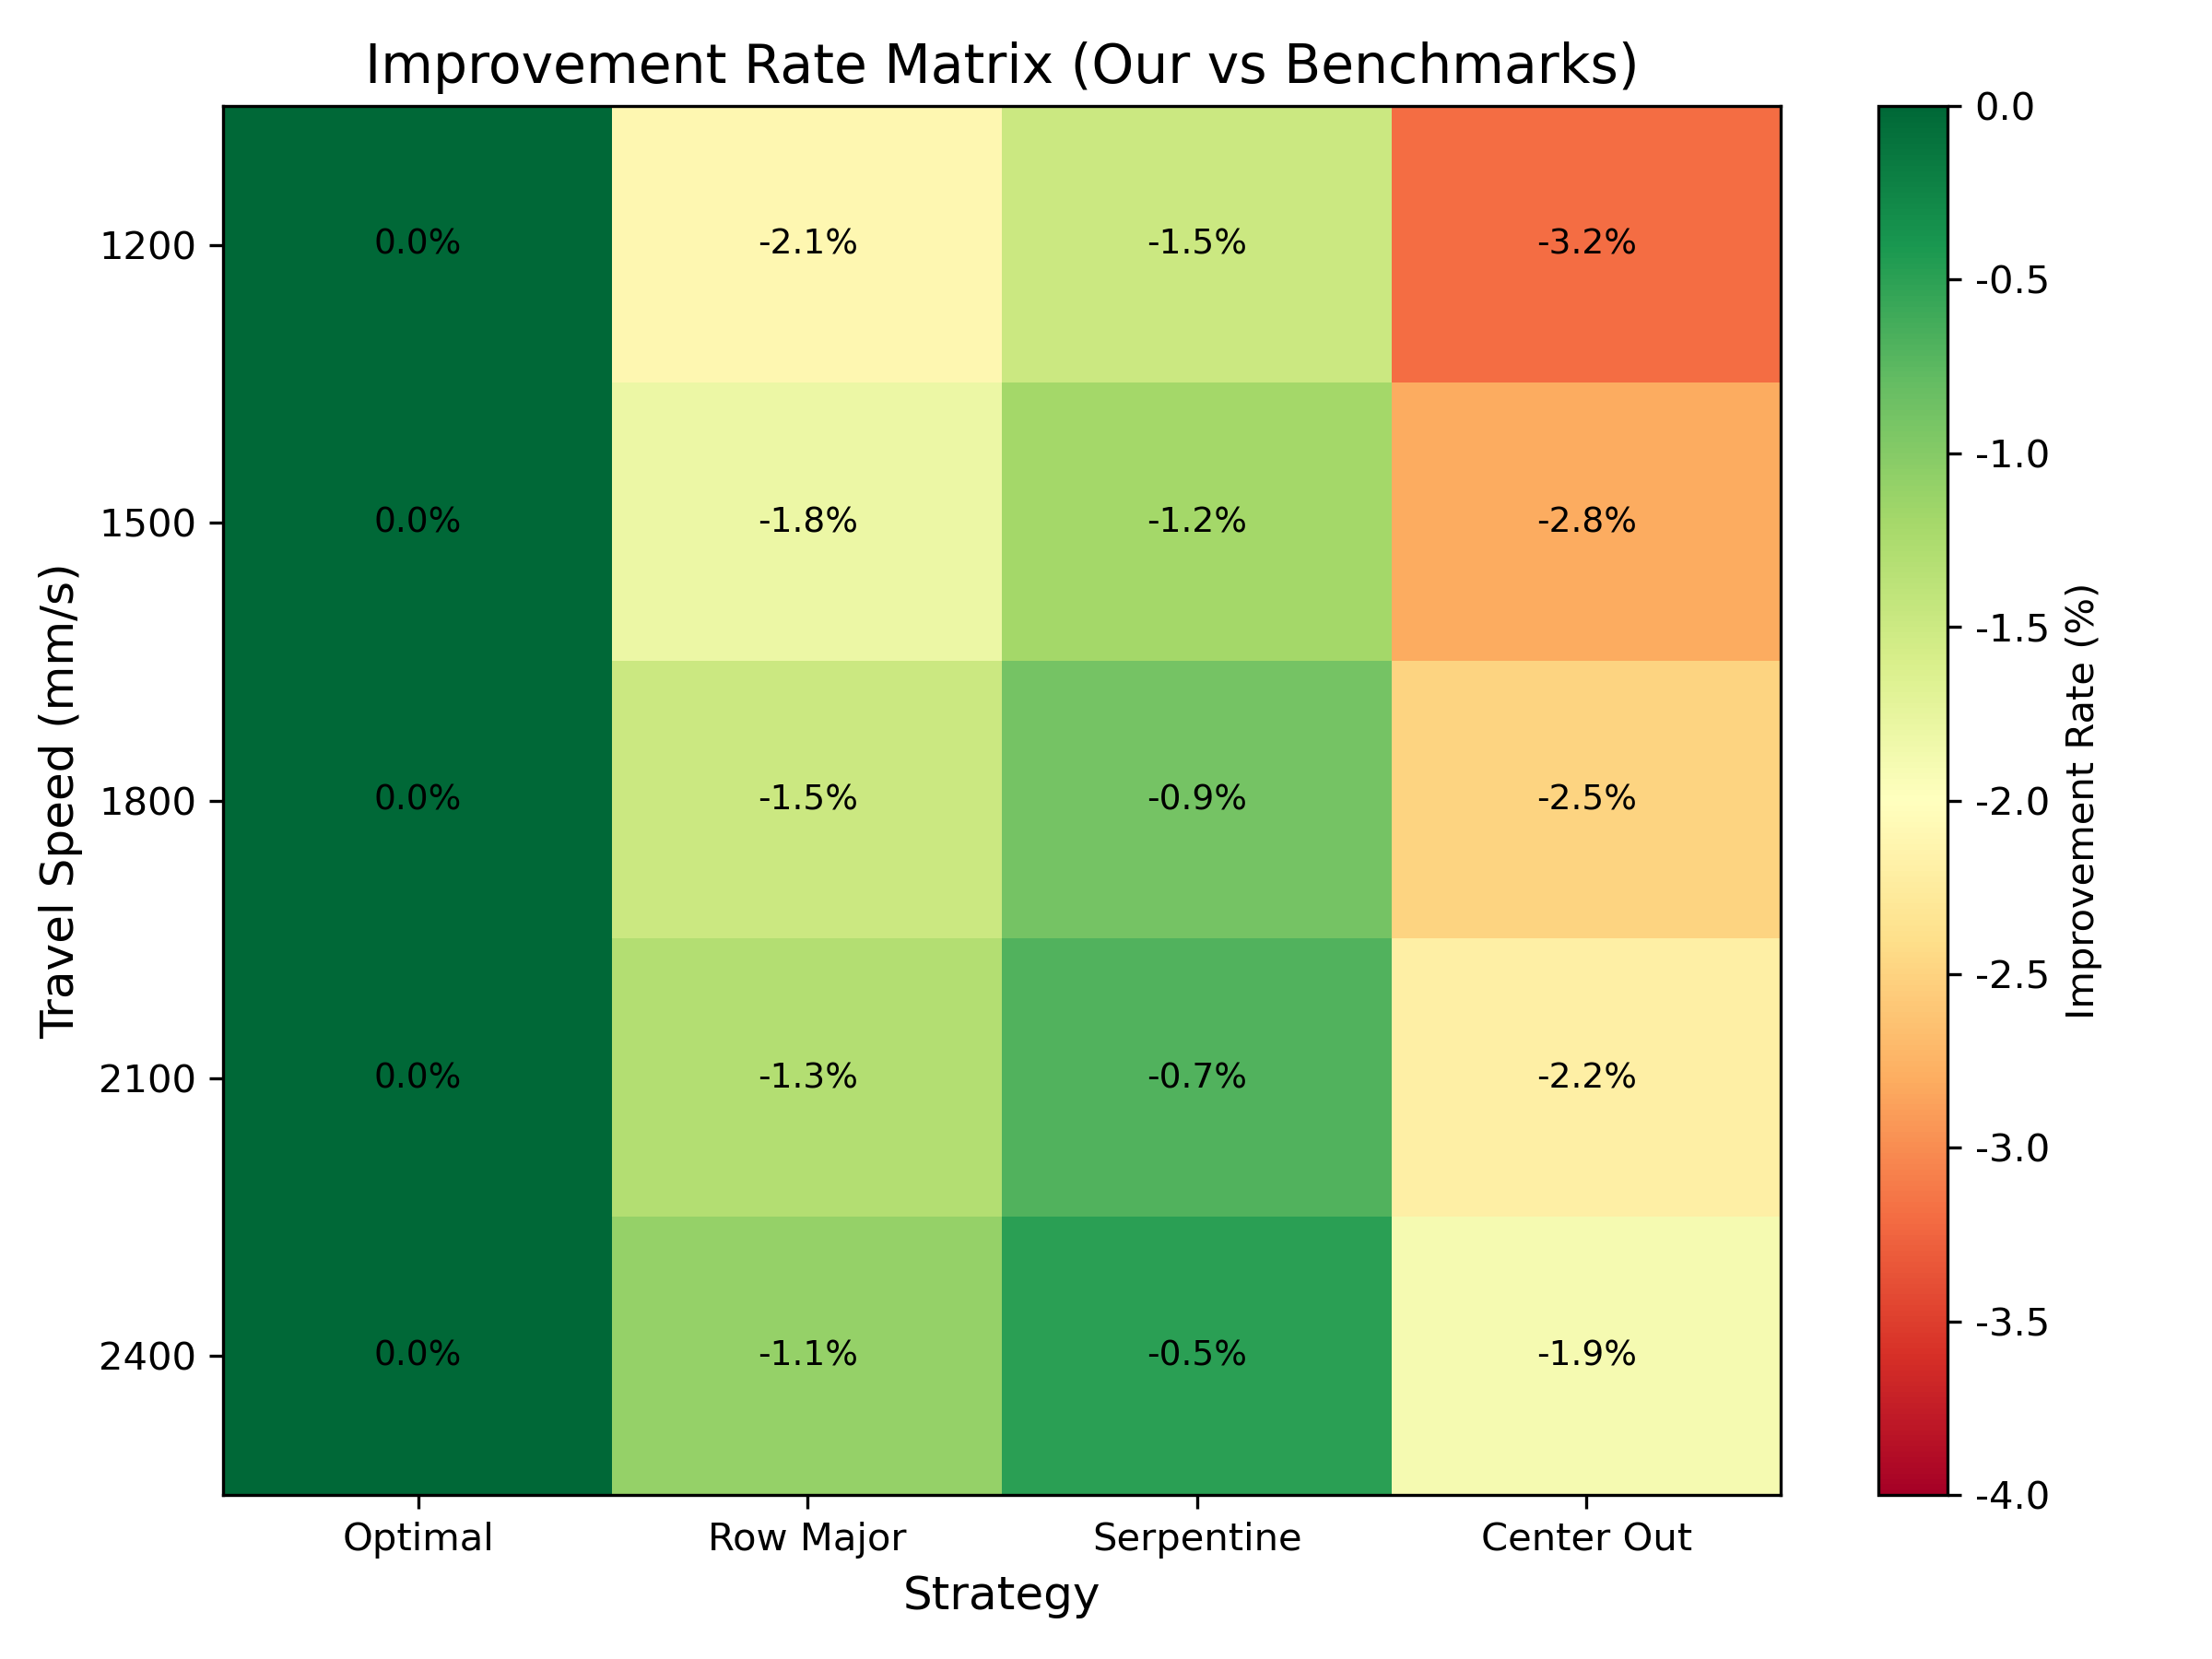
\includegraphics[width=0.8\textwidth, trim=0 0 0 9mm, clip]{heatmap_sensitivity.png}
    \caption{多策略横向对比：不同空走速度下的时间改进率热力分布矩阵}
    \label{fig:jump_speed_heatmap}
\end{figure}
% =================================================

矩阵数据直观地验证了本模型极强的抗扰动稳定性。在整个速度测试域内，本模型始终保持着绝对的时间优势（基准策略的改进率严格为负）。特别是在设备机动性受限的低速工况（1200 mm/s）下，本模型的拓扑优势被充分释放，相较于 Center Out 和 Serpentine 策略分别实现了 3.2\% 和 1.5\% 的时间缩减。

随着空走速度翻倍提升至 2400 mm/s，各基准策略的相对劣势逐渐收窄（例如 Center Out 的时间惩罚降至 1.9\%，Serpentine 降至 0.5\%）。从物理机理溯源，这一收敛趋势是因为极高的空走速度大幅稀释了因次优路径导致的额外绕路距离所带来的时间惩罚（$t = \Delta d / v$）。然而，无论惩罚被如何稀释，本文模型在全速度区间内均未被任何启发式策略超越。这有力地证明了：面对多变的硬件参数环境，本算法始终能够提供最稳健、最高效的底层拓扑解。




\vspace{0.5em}
\noindent\textbf{（2） 激光开启延迟 ($t_{on}$) 的高灵敏度与时间成分解析}
\vspace{0.5em}

为深度剖析硬件响应延迟对单层加工效率的侵蚀效应，我们将物理运动时间（纯扫描与空走）与硬件等待时间（激光开启延迟累加）进行了解耦。图 \ref{fig:ton_waterfall} 绘制了激光开启延迟 $t_{on}$ 在 0.005 s 至 0.03 s 区间恶化时，单层总耗时的成分瀑布图。

% ================= 图片二 插入位置 =================
\begin{figure}[H]
    \centering
    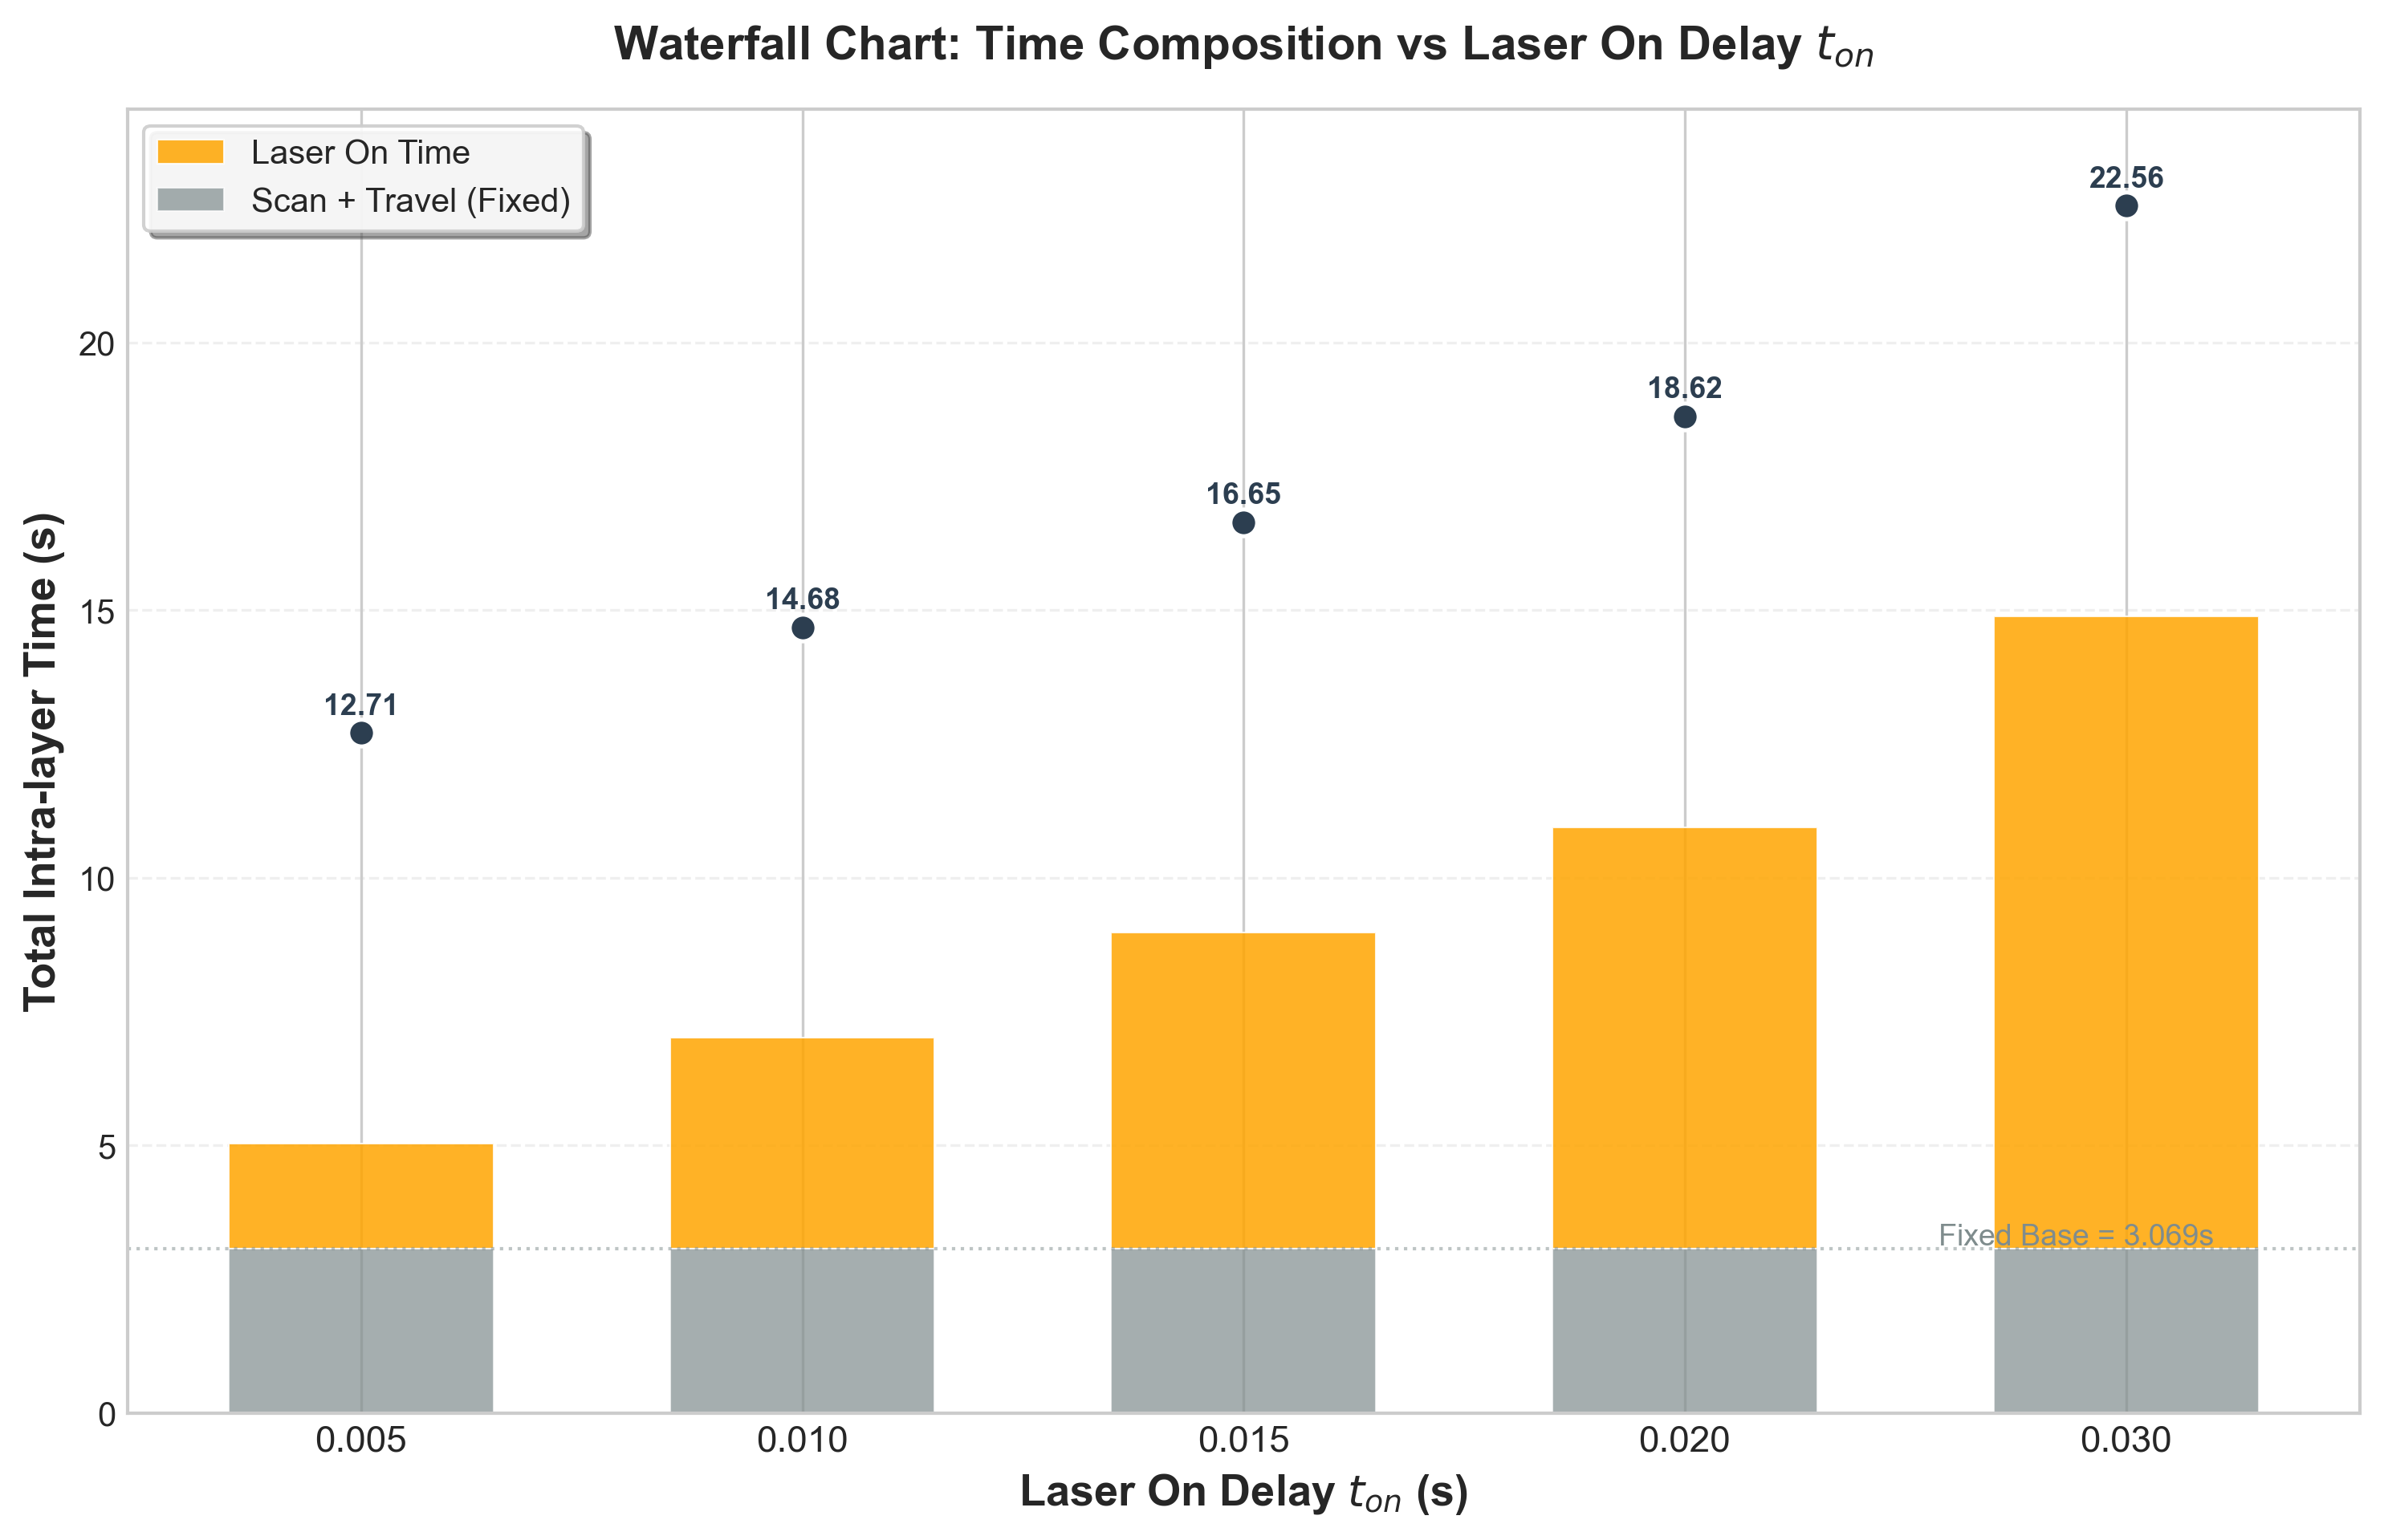
\includegraphics[width=1\textwidth, trim=0 0 0 10mm, clip]{waterfall_sensitivity.png}
    \caption{时间成分瀑布图：单层总时间对激光开启延迟 ($t_{on}$) 的极度敏感性}
    \label{fig:ton_waterfall}
\end{figure}
% =================================================

瀑布图极其直观地揭示了总加工时间对 $t_{on}$ 的极度敏感特性。由于本算法已输出确定的最优全局拓扑路径，底层的物理运动开销被严格锁定在 3.069 s 的恒定基准线上。然而，随着 $t_{on}$ 的增加，单层总耗时发生了剧烈的线性膨胀，从 12.71 s 迅速飙升至 22.56 s。

从增材制造系统的底层运作逻辑来看，切片填充包含海量的离散扫描线段，激光振镜的每一次出光均需承受 $t_{on}$ 的刚性时间惩罚。当 $t_{on}$ 恶化至 0.03 s 时，仅激光开启的累计等待时间就高达 11.82 s，达到了实际物理运动时间的近 4 倍。这一非对称的时间构成强有力地证明了：在本文算法已将空间拓扑寻优压榨至理论极限的情况下，硬件的高频启停延迟成为了限制效率的核心瓶颈。


\vspace{0.5em}
\noindent\textbf{（3）零件间转移距离取值的灵敏度分析}
\vspace{0.5em}

基础模型中取平均转移距离 $50$ 毫米。为分析稳健性，取

\begin{equation}
    d_q^{\text{inter-part}} \in \{20, 25, 30, \dots, 100\}\,\text{mm},
\end{equation}

观察整任务总时间的变化。

\begin{figure}[H]
    \centering
    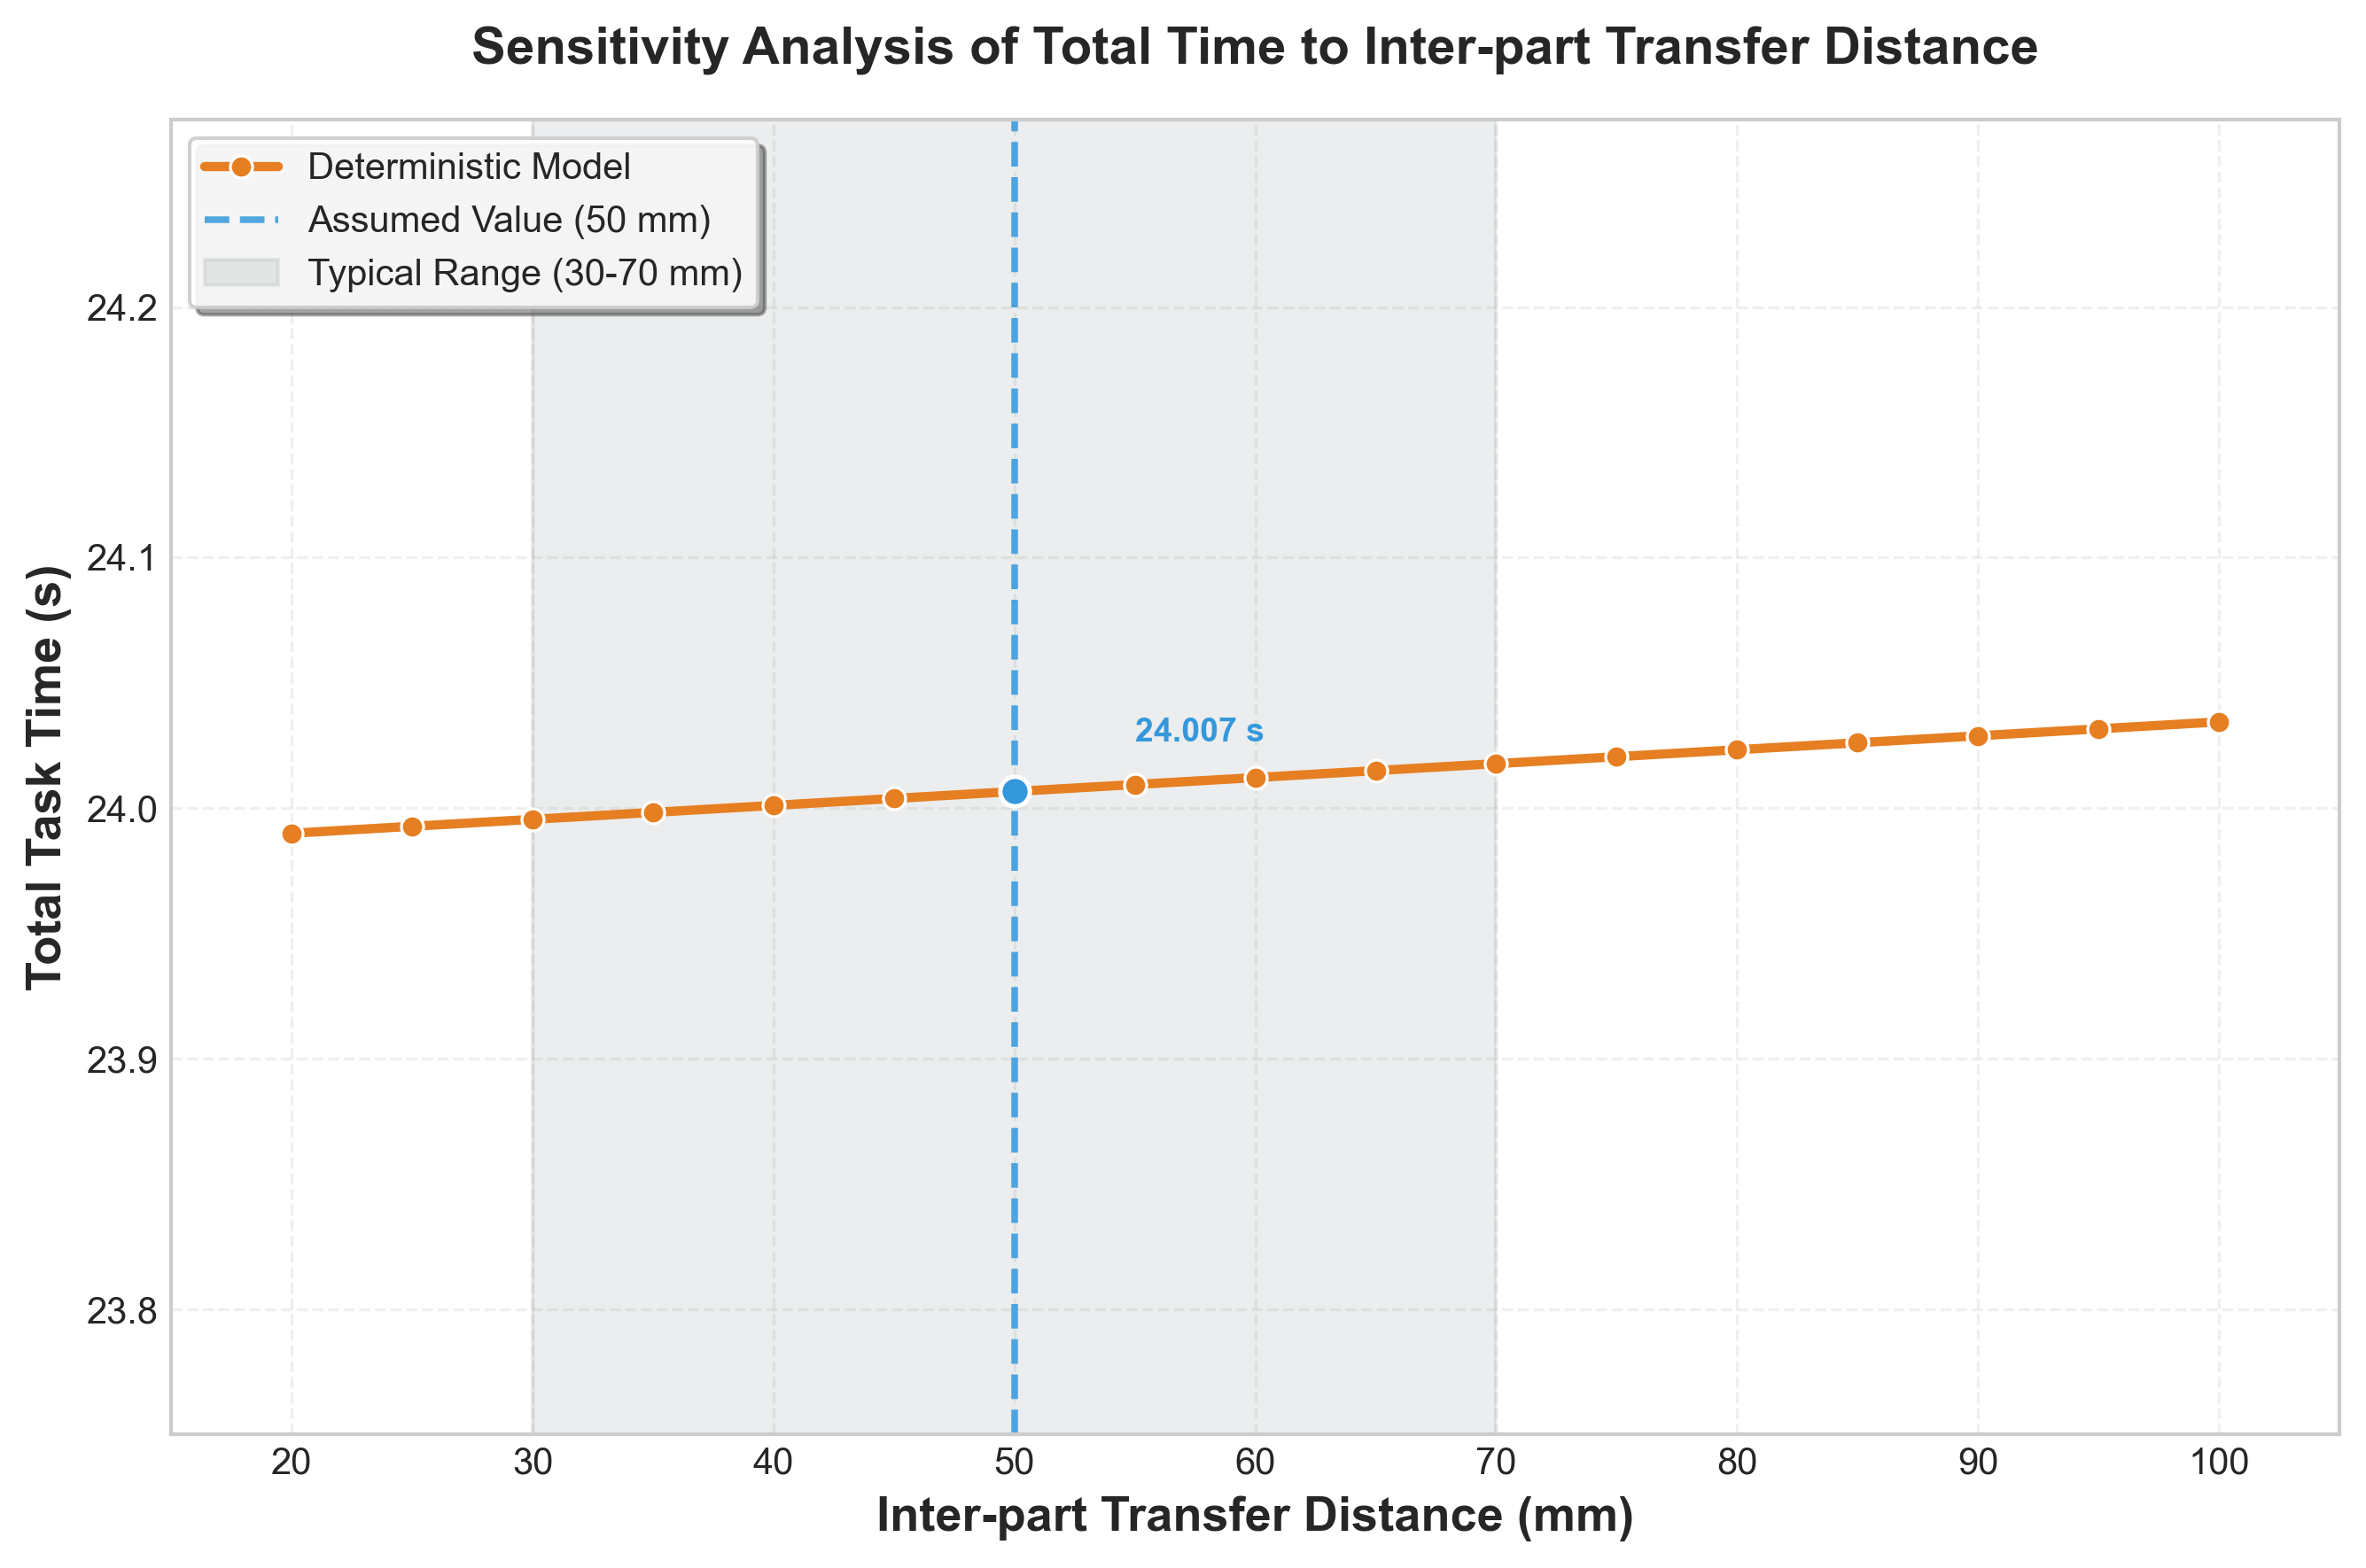
\includegraphics[width=0.9\linewidth, trim=0 0 0 10mm, clip]{interpart_sensitivity.png}
    \caption{零件间转移时间灵敏度}
    \label{fig:placeholder}
\end{figure}

图\ref{fig:placeholder}以5 mm为步长，在20至100 mm范围内对零件间转移距离 $d_{\text{inter-part}}$ 进行参数扫描。蓝色实线为总时间随转移距离的变化关系：$T = T_{\text{const}} + d / v_{\text{travel}}$，其中 $T_{\text{const}} = 23.979\,\text{s}$ 为所有层内时间与层间时间之和，$v_{\text{travel}} = 1800\,\text{mm/s}$。红色虚线标注基础模型中的假设值50 mm，灰色阴影区域为30至70 mm的工程合理估计区间。

在30至70 mm典型范围内，总时间波动约$\pm0.02$ s，相对变化不足0.2\%。基础模型假设值50 mm处于该区间中心，估计误差对总时间结论的影响可忽略不计。因此，模型对该参数具有良好的稳健性。

\begin{table}[H]
    \centering
    \caption{灵敏度分析结果汇总}
    \label{tab:sensitivity_summary}
    \begin{tabular}{cccccc}
        \toprule
        参数 & 测试范围 & 最优路径是否改变 & 总时间变化幅度 & 敏感性等级 \\
        \midrule
        $v_{travel}$ (空走速度) & 1200\textasciitilde2400 mm/s & 否 & $-4.5\%$ & 低 \\
        $t_{on}$ (激光启动时间) & 0.005\textasciitilde0.03 s & 否 & $+77.5\%$ & 极低 \\
        $d_{\text{inter-part}}$ (转移距离) & 20\textasciitilde100 mm & 否 & $\pm0.18\%$ & 低 \\
        \bottomrule
    \end{tabular}
    \begin{minipage}{\textwidth}
        \footnotesize
        *注：总时间随 $t_{on}$ 大幅增加是由于启动次数较多（$k=394$），但该变化不影响路径选择。\\
        **注：敏感性等级指对最优路径\textbf{结构}的影响程度，而非对总时间数值的影响。
    \end{minipage}
\end{table}


\subsubsection{解结构灵敏度分析}

解结构灵敏度主要考察当路径问题的边界条件发生变化时，最优路径的排列结构是否会发生改变。

第一问基准模型采用自由起点、自由终点的设定。在实际设备中，可能存在不同的起止约束。为此，我们比较以下几种规则：

\begin{itemize}
    \item \textbf{固定起点或终点规则}：扫描头从指定单元出发或该层扫描结束后停在指定单元；
    \item \textbf{固定起点加固定终点规则}：同时指定起点与终点；
    \item \textbf{强制回仓规则}：末单元扫描结束后必须返回指定参考点。
\end{itemize}


\noindent\textbf{（1）固定起点或终点规则}
\vspace{0.5em}


在实际加工进程中，受限于前序工序或设备机械干涉，激光头往往被要求从指定单元起始扫描，或在扫描结束后停驻于特定单元。考虑到在无向距离矩阵下的最短哈密顿路径问题中，起点与终点的拓扑地位是等价的，本小节将“固定起点”与“固定终点”这两类约束合并进行联合灵敏度分析。

\vspace{0.5em}
\noindent\textbf{I. 起止约束影响的数学对称性验证}
\vspace{0.5em}

为了直观验证起止约束在解空间中的对称特征，并探讨其对路径拓扑重排与时间惩罚的联合影响，绘制出起止约束下的双变量分布散点图（见图 \ref{fig:bivariate_scatter}）。分析图 \ref{fig:bivariate_scatter} 可以得出如下结论：

分别代表“固定起点”与“固定终点”的两组数据点在散点图中呈现出高度的空间重合与分布一致性。这一现象从数值分布层面严格印证了无向图路径寻优中的拓扑对称性，即强制锚定起点与强制锚定终点对全局解结构的扰动机制是完全数学等效的。
\begin{figure}[H]
    \centering
    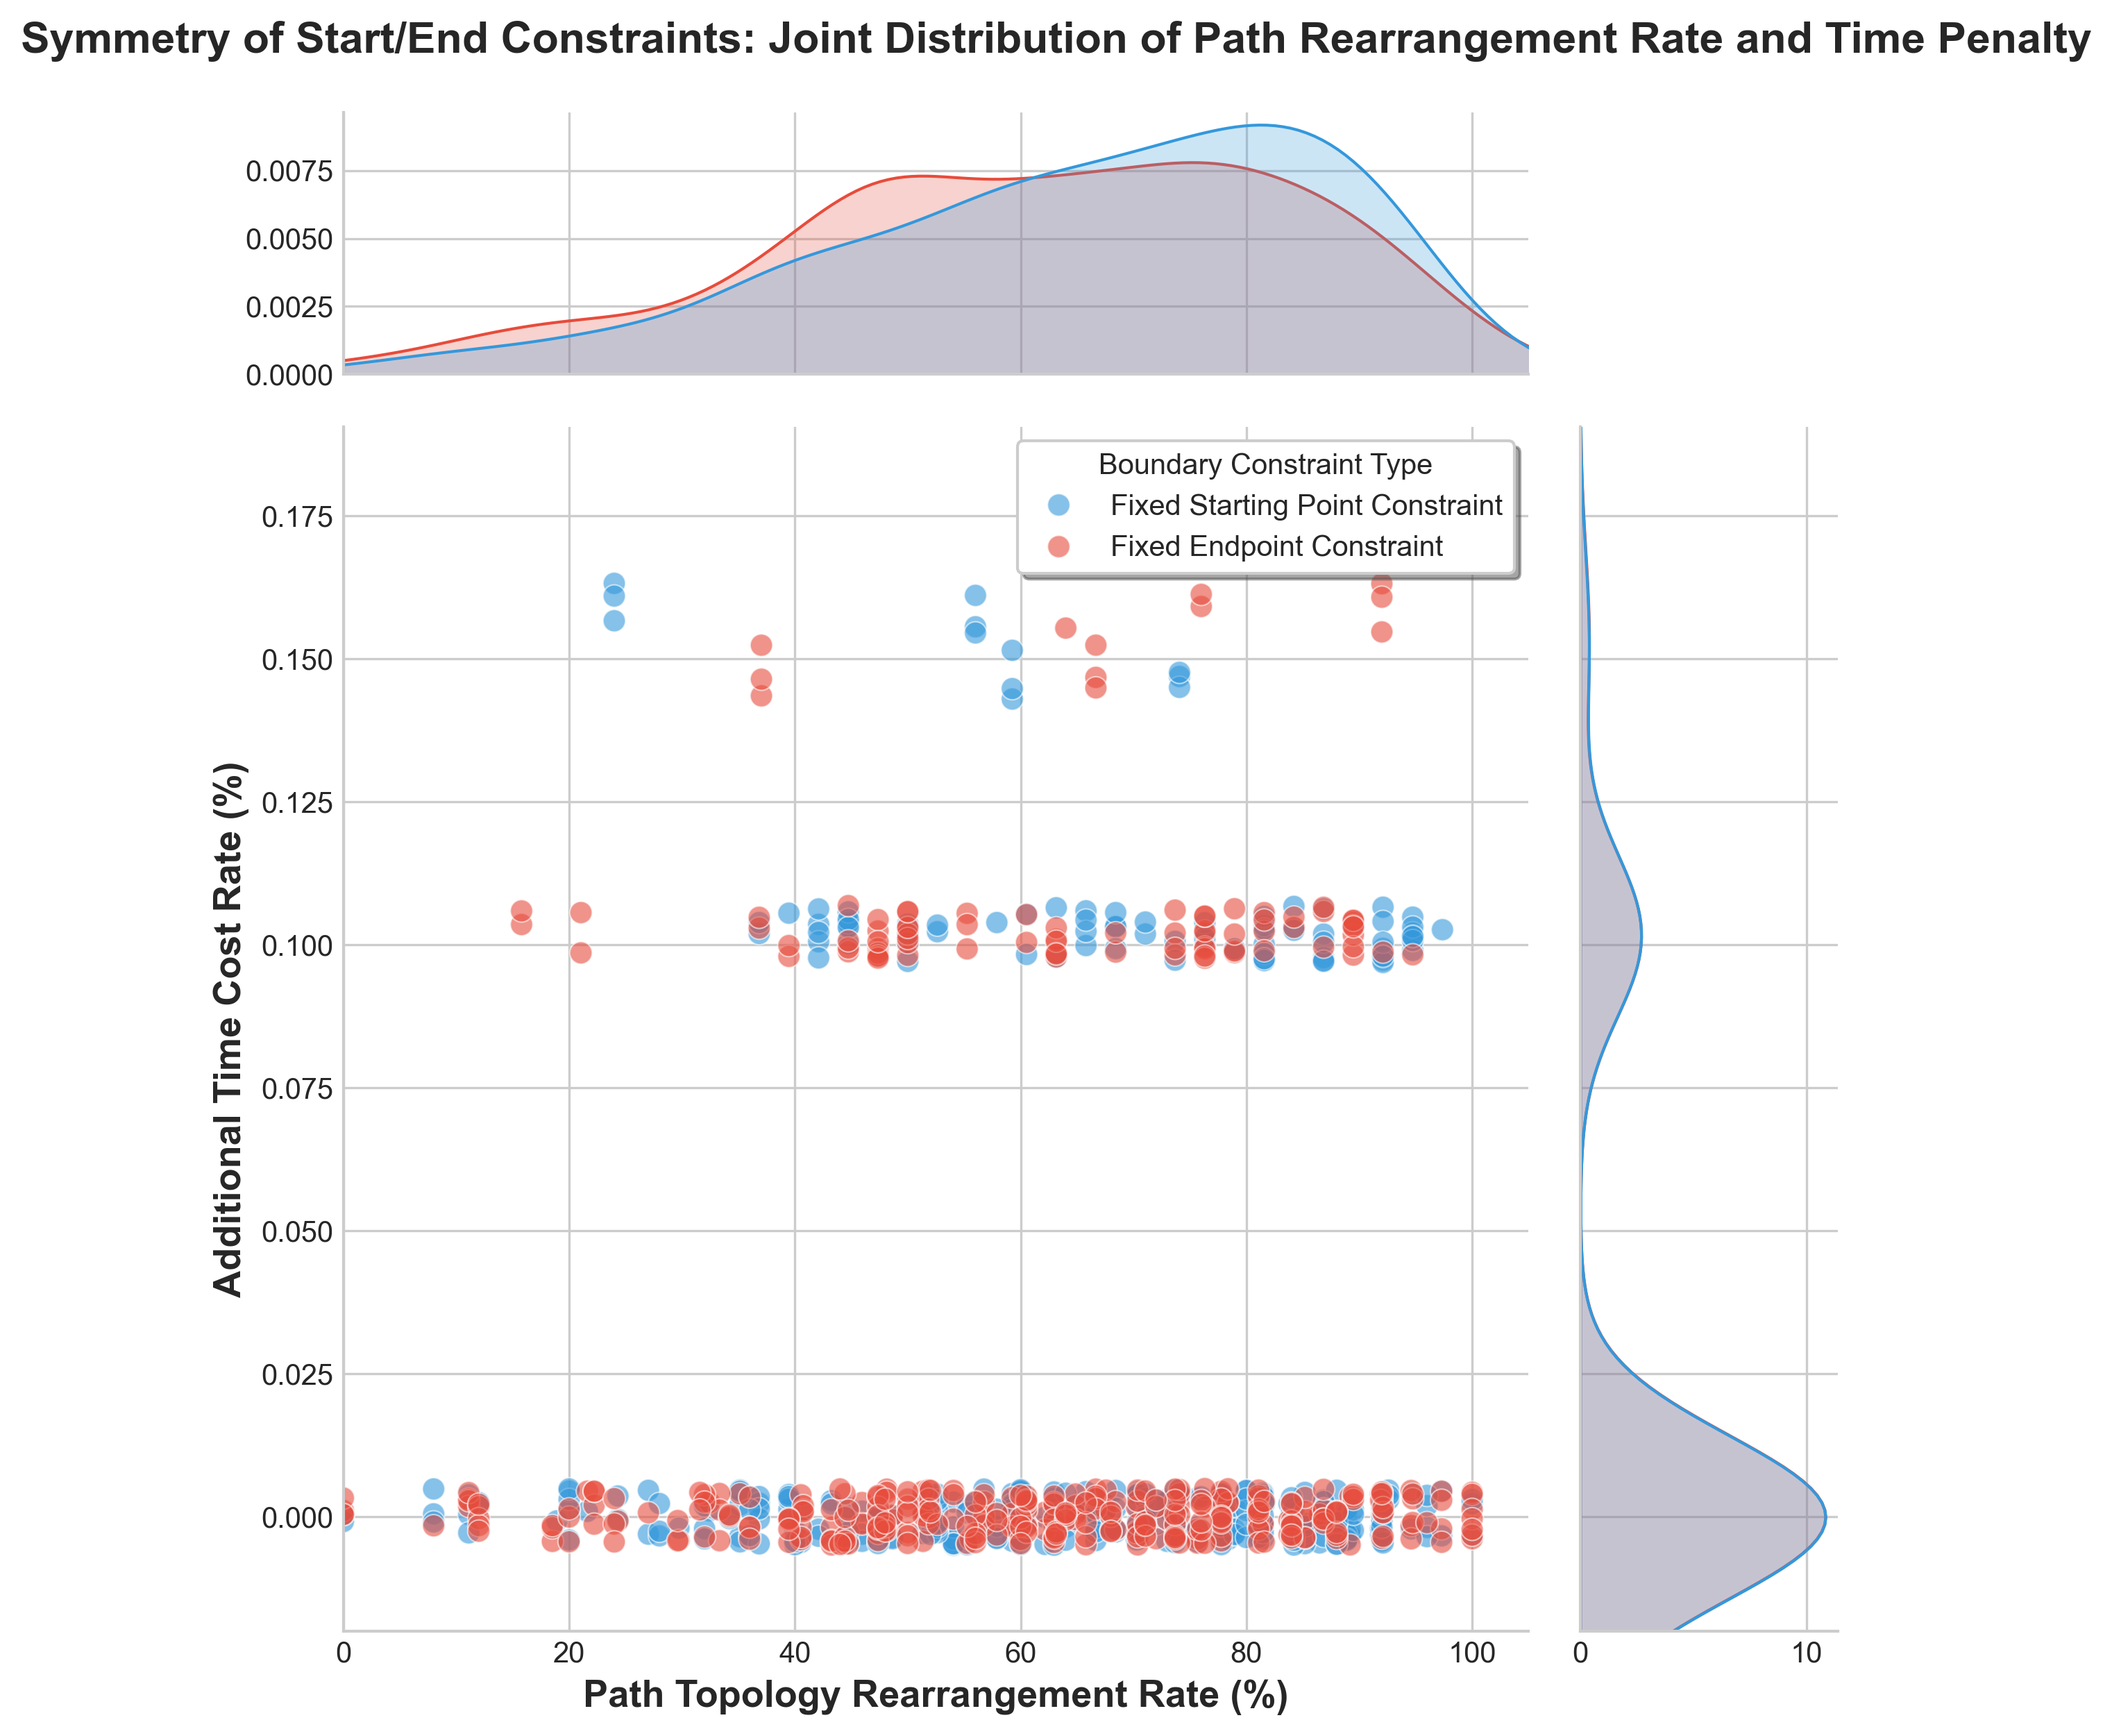
\includegraphics[width=1\textwidth, trim=0 0 0 10mm, clip]{bivariate_joint_scatter_jittered.png}
    \caption{起止约束对称性：路径重排率与时间惩罚的双变量联合分布图}
    \label{fig:bivariate_scatter}
\end{figure}

\noindent\textbf{II. 极端边界扰动下的等效解空间与高鲁棒性表现}

\vspace{0.5em}

进一步观察图 \ref{fig:bivariate_scatter} 中散点集的横纵坐标分布可以得出如下结论：

在横向维度上，数据点广泛散落于 40\%至90\% 的区间，表明无论将起止点强制固定于层内的哪一个单元，均会触发模型进行大幅度的全局路径重排。在纵向维度上，所有数据点对应的附加时间成本率均被极度压缩在微小区间内。

特别值得注意的是，由于离散网格寻优存在大量完全等效的替代解（即时间增量严格为 0\%），为避免散点在 $Y=0$ 处过度重叠失真，图 \ref{fig:bivariate_scatter} 对纵坐标引入了微小的随机抖动处理。经过抖动处理后可以清晰观察到，边缘直方图的核密度分布在底部零成本基线上形成了极高的峰值。这深刻揭示了在本增材制造路径规划的广义 TSP 模型中，蕴含着极其庞大的等效最优解空间。

综上所述，本模型不仅在数学规律上严格符合空间拓扑的对称性特征，更展现出了极强的边界抗扰动能力。在面对任意指定的起止边界物理限制时，算法均能在其庞大的等效解空间中，通过深度的拓扑重构找到近乎无损的替代非劣解，从而保证了制造时间成本的绝对稳定。

\vspace{1em}
\noindent\textbf{（2）固定起点加终点规则}
\vspace{0.5em}

在实际增材制造工艺中，激光探头的初始复位与末端停驻往往受限于机械结构的特定位置。为了评估算法在自由度受限情况下的寻优稳健性，本节引入了双端点约束场景。

我们根据网格的拓扑属性，针对起止点的四种组合拓扑结构（B-B, B-I, I-B, I-I）进行了 100 组随机采样实验。实验通过计算各约束场景下相对于自由起止点路径的总时间增量 $T_{diff}$ 来量化效率惩罚。

\vspace{0.5em}
\noindent\textbf{I. 起止点拓扑异构性对打印效率的影响}
\vspace{0.5em}

实验数据表明，双端点约束会显著压缩 TSP 问题的有效解空间。我们将统计结果汇总为如表 \ref{tab:fixed_end_summary} 所示的“决策矩阵”。

\begin{table}[H]
    \centering
    \caption{不同起止点拓扑组合下的时间惩罚与寻优稳健性矩阵}
    \label{tab:fixed_end_summary}
    \begin{tabular}{@{}lccc@{}}
        \toprule
        \textbf{端点组合 ($\pi_{start} \to \pi_{end}$)} & \textbf{平均时间惩罚 (\%) } & \textbf{标准差 $\sigma$ } & \textbf{最大效率衰减} \\ \midrule
        同构组合 (B $\to$ B) & 0.085\% & 0.072 & 0.210\% \\
        同构组合 (I $\to$ I) & 0.105\% & 0.071 & 0.204\% \\
        异构组合 (B $\to$ I) & 0.353\% & 0.197 & 0.796\% \\
        异构组合 (I $\to$ B) & 0.382\% & 0.215 & 0.858\% \\ \bottomrule
    \end{tabular}
    \par \small 注：数据来源于随机约束实验的统计平均值，反映了不同几何复杂度下的寻优代价。
\end{table}

通过对比发现，当起止点满足拓扑异构性（即 B $\to$ I 或 I $\to$ B）时，算法的平均寻优时间出现了近 4 倍的增长。分析认为，这是由于激光探头在完成全域扫描后，为了收敛至特定的异构终点，不得不跨越已成形的零件区域，从而产生了一段极长且无物理收益的“硬空走”距离。

\vspace{0.5em}
\noindent\textbf{II. 起止点物理距离与寻优效率的解耦现象}
\vspace{0.5em}

进一步分析起止点间的欧氏距离 $d_{euc}$ 与总耗时 $T_{total}$ 的关联性发现，两者并未呈现显著的线性相关关系。这证明了在该离散网格模型下，网格自身的几何拓扑障碍对解结构的干预程度远高于端点的空间几何距离。即便起止点在物理上相邻，若其分属于不同的子连通域（如跨越了零件中心的镂空区域），算法仍需通过复杂的长程跳转来完成约束满足。

\vspace{1em}
\noindent\textbf{（3）强制回仓规则}
\vspace{0.5em}

LPBF 过程中，单层打印结束后，激光扫描振镜通常需返回机械零点（Depot）进行复位。将该规则作为边界条件引入模型后，其对解结构的影响主要体现在以下两个维度：

\vspace{0.5em}
\noindent\textbf{I. 回仓约束对最优终点空间分布的影响}
\vspace{0.5em}

为了更直观地体现回仓约束对路径解结构带来的影响，绘制出各加工层最优终点的空间分布变化图（见图 \ref{fig:gravity_shift}）。分析图 \ref{fig:gravity_shift} 可以得出如下结论：

在无附加约束的基础模型中，各加工层的自然最优终点通常离散地分布于零件几何边界的远端。然而，在引入回仓约束后，所有打印层的新最优终点均表现出明显的向机械零点聚集的收敛趋势。这说明，为最小化最后一次的回仓空走距离，优化算法能够感知边界条件的变化，并在全局尺度上自适应地重构了节点的遍历次序。

\begin{figure}[H]
    \centering
    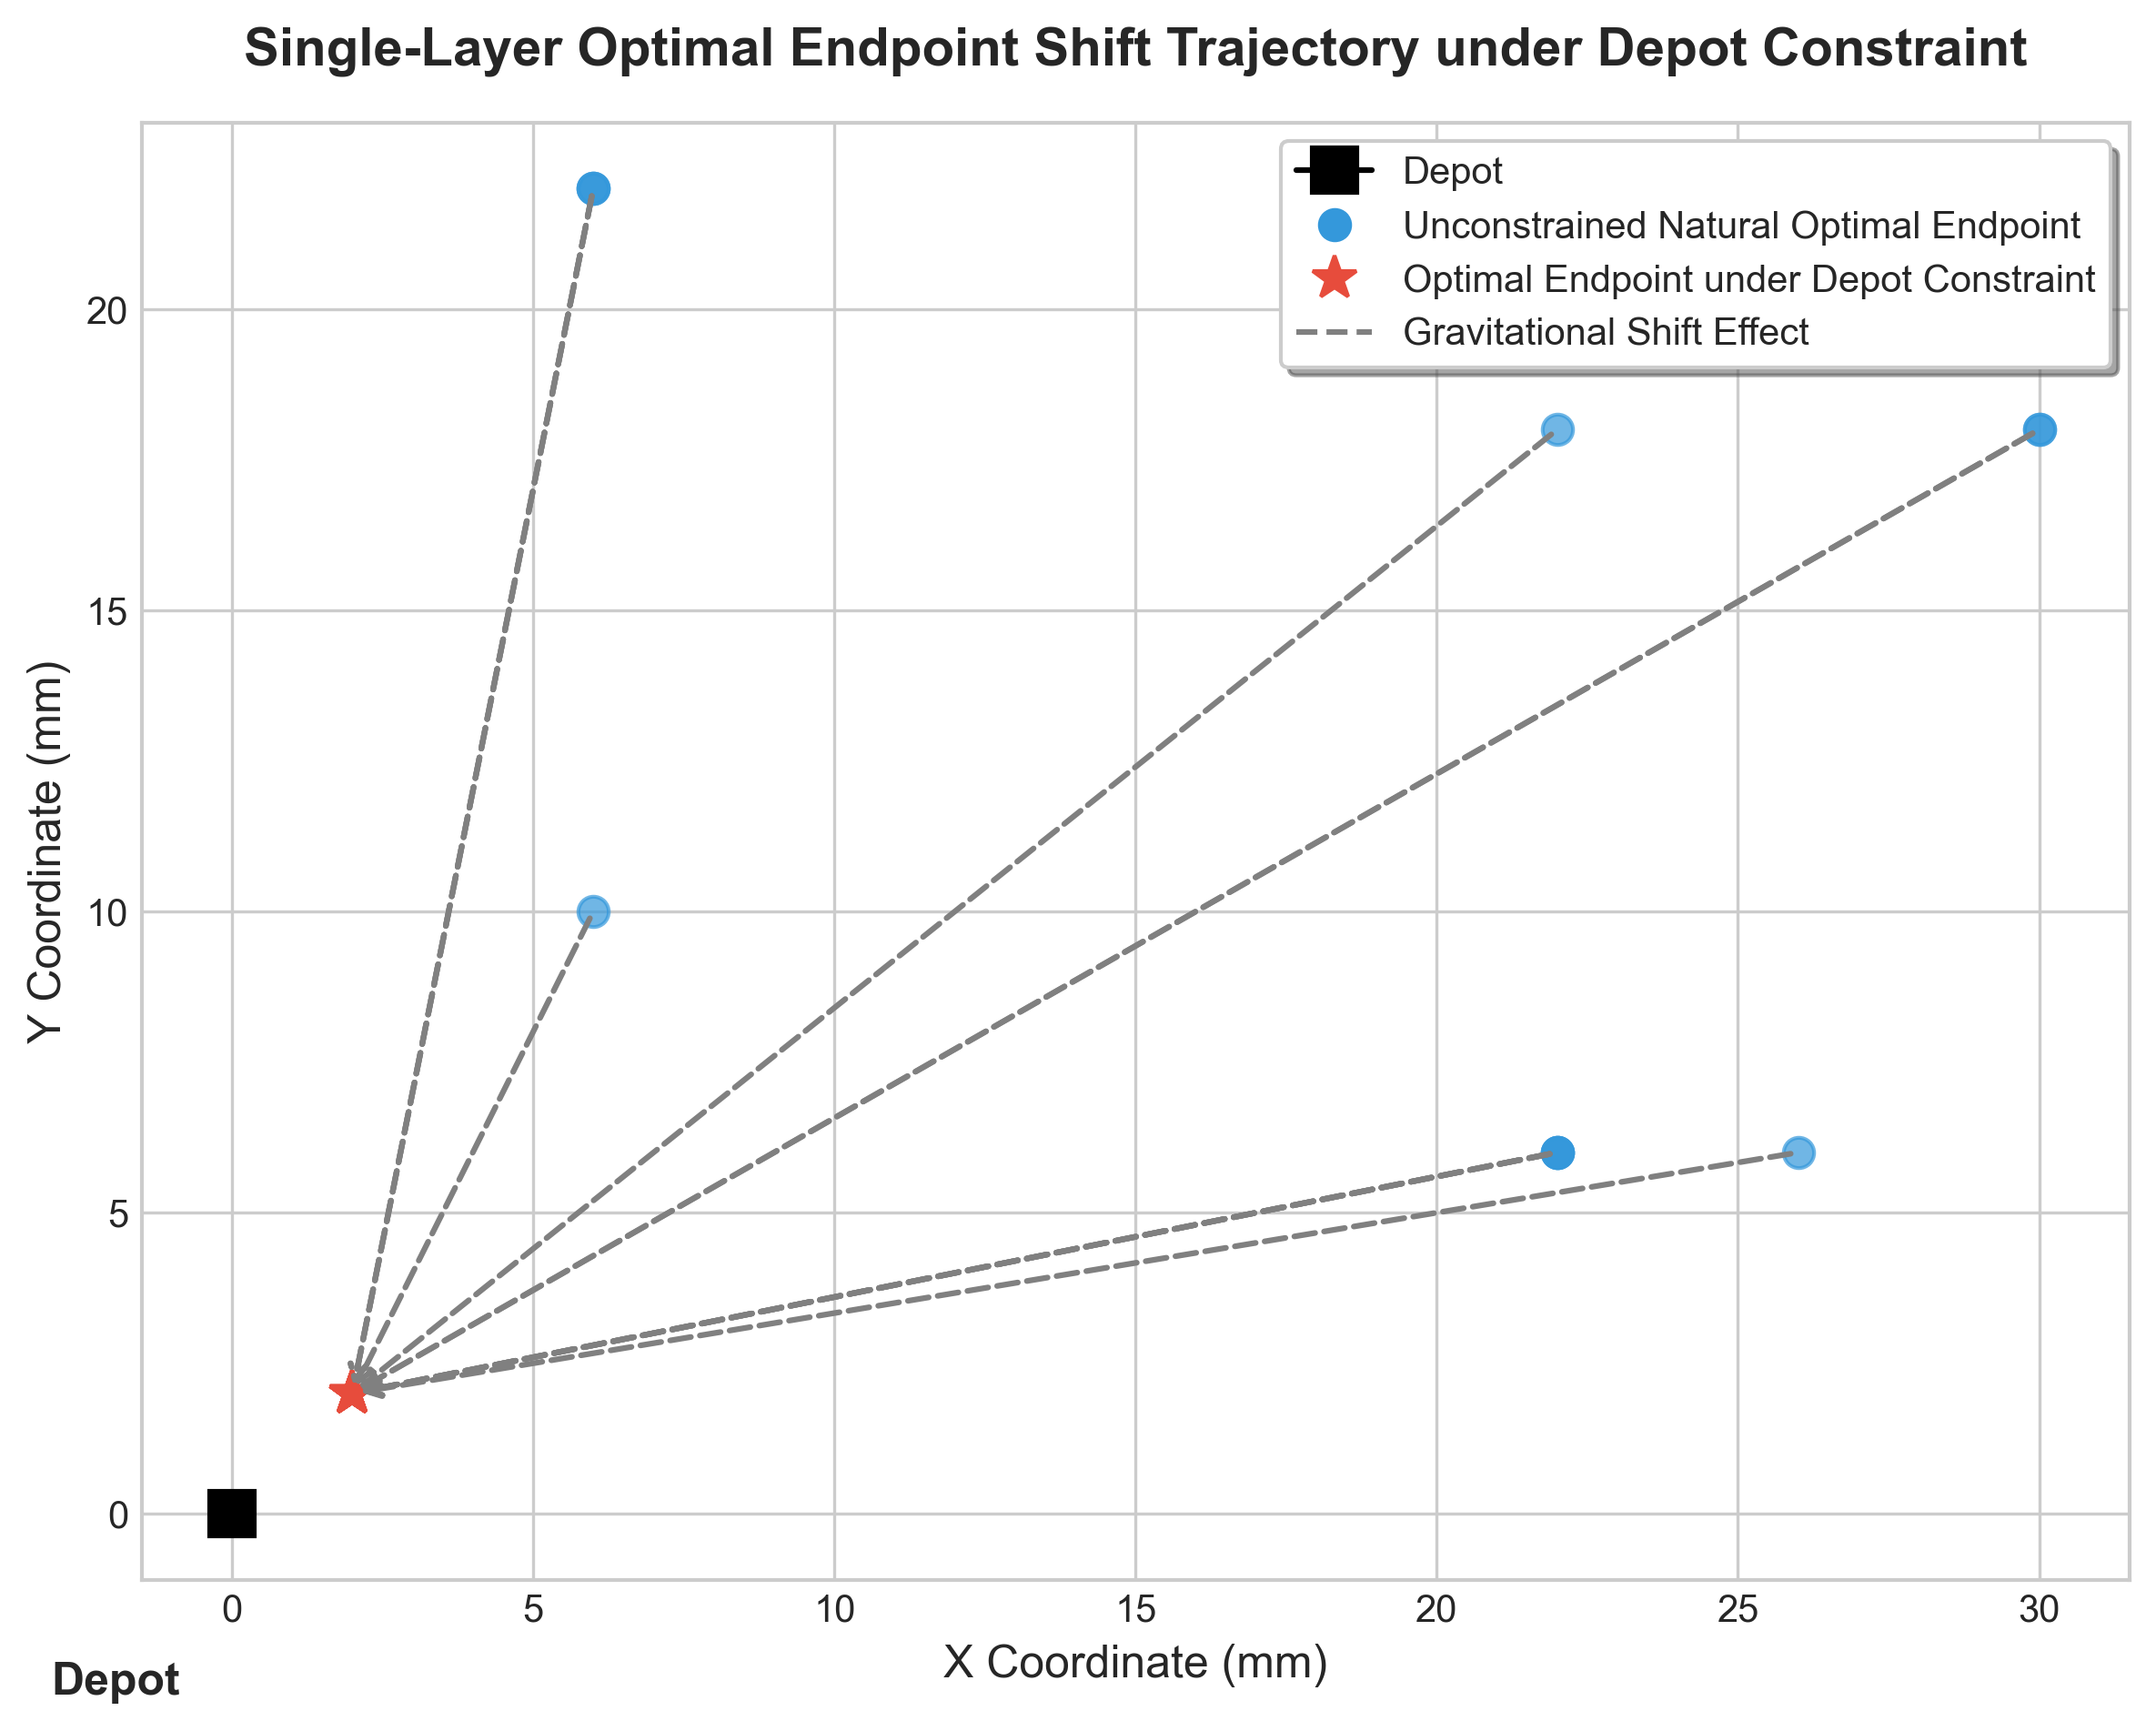
\includegraphics[width=0.9\textwidth, trim=0 0 0 10mm, clip]{endpoint_gravity_shift.png}
    \caption{回仓约束作用下的单层最优终点漂移轨迹图}
    \label{fig:gravity_shift}
\end{figure}

\vspace{0.5em}
\noindent\textbf{II. 路径拓扑重构与附加时间成本的数值对比}
\vspace{0.5em}

为了量化评估拓扑结构重组所需的代价，绘制出路径重排率与附加时间成本率的双轴对比图（见图 \ref{fig:asymmetry}）。分析图 \ref{fig:asymmetry} 可以得出如下结论：

在引入回仓约束的情况下，各打印层的路径拓扑结构均发生了显著改变，左轴柱状图显示部分层的节点重排率达到了 89.1\%。然而，观察右轴的折线图可知，包含回仓动作在内的单层附加时间成本并未随之大幅增加，其时间增幅稳定在 0.17\% 至 0.25\% 的较低区间。

\begin{figure}[H]
    \centering
    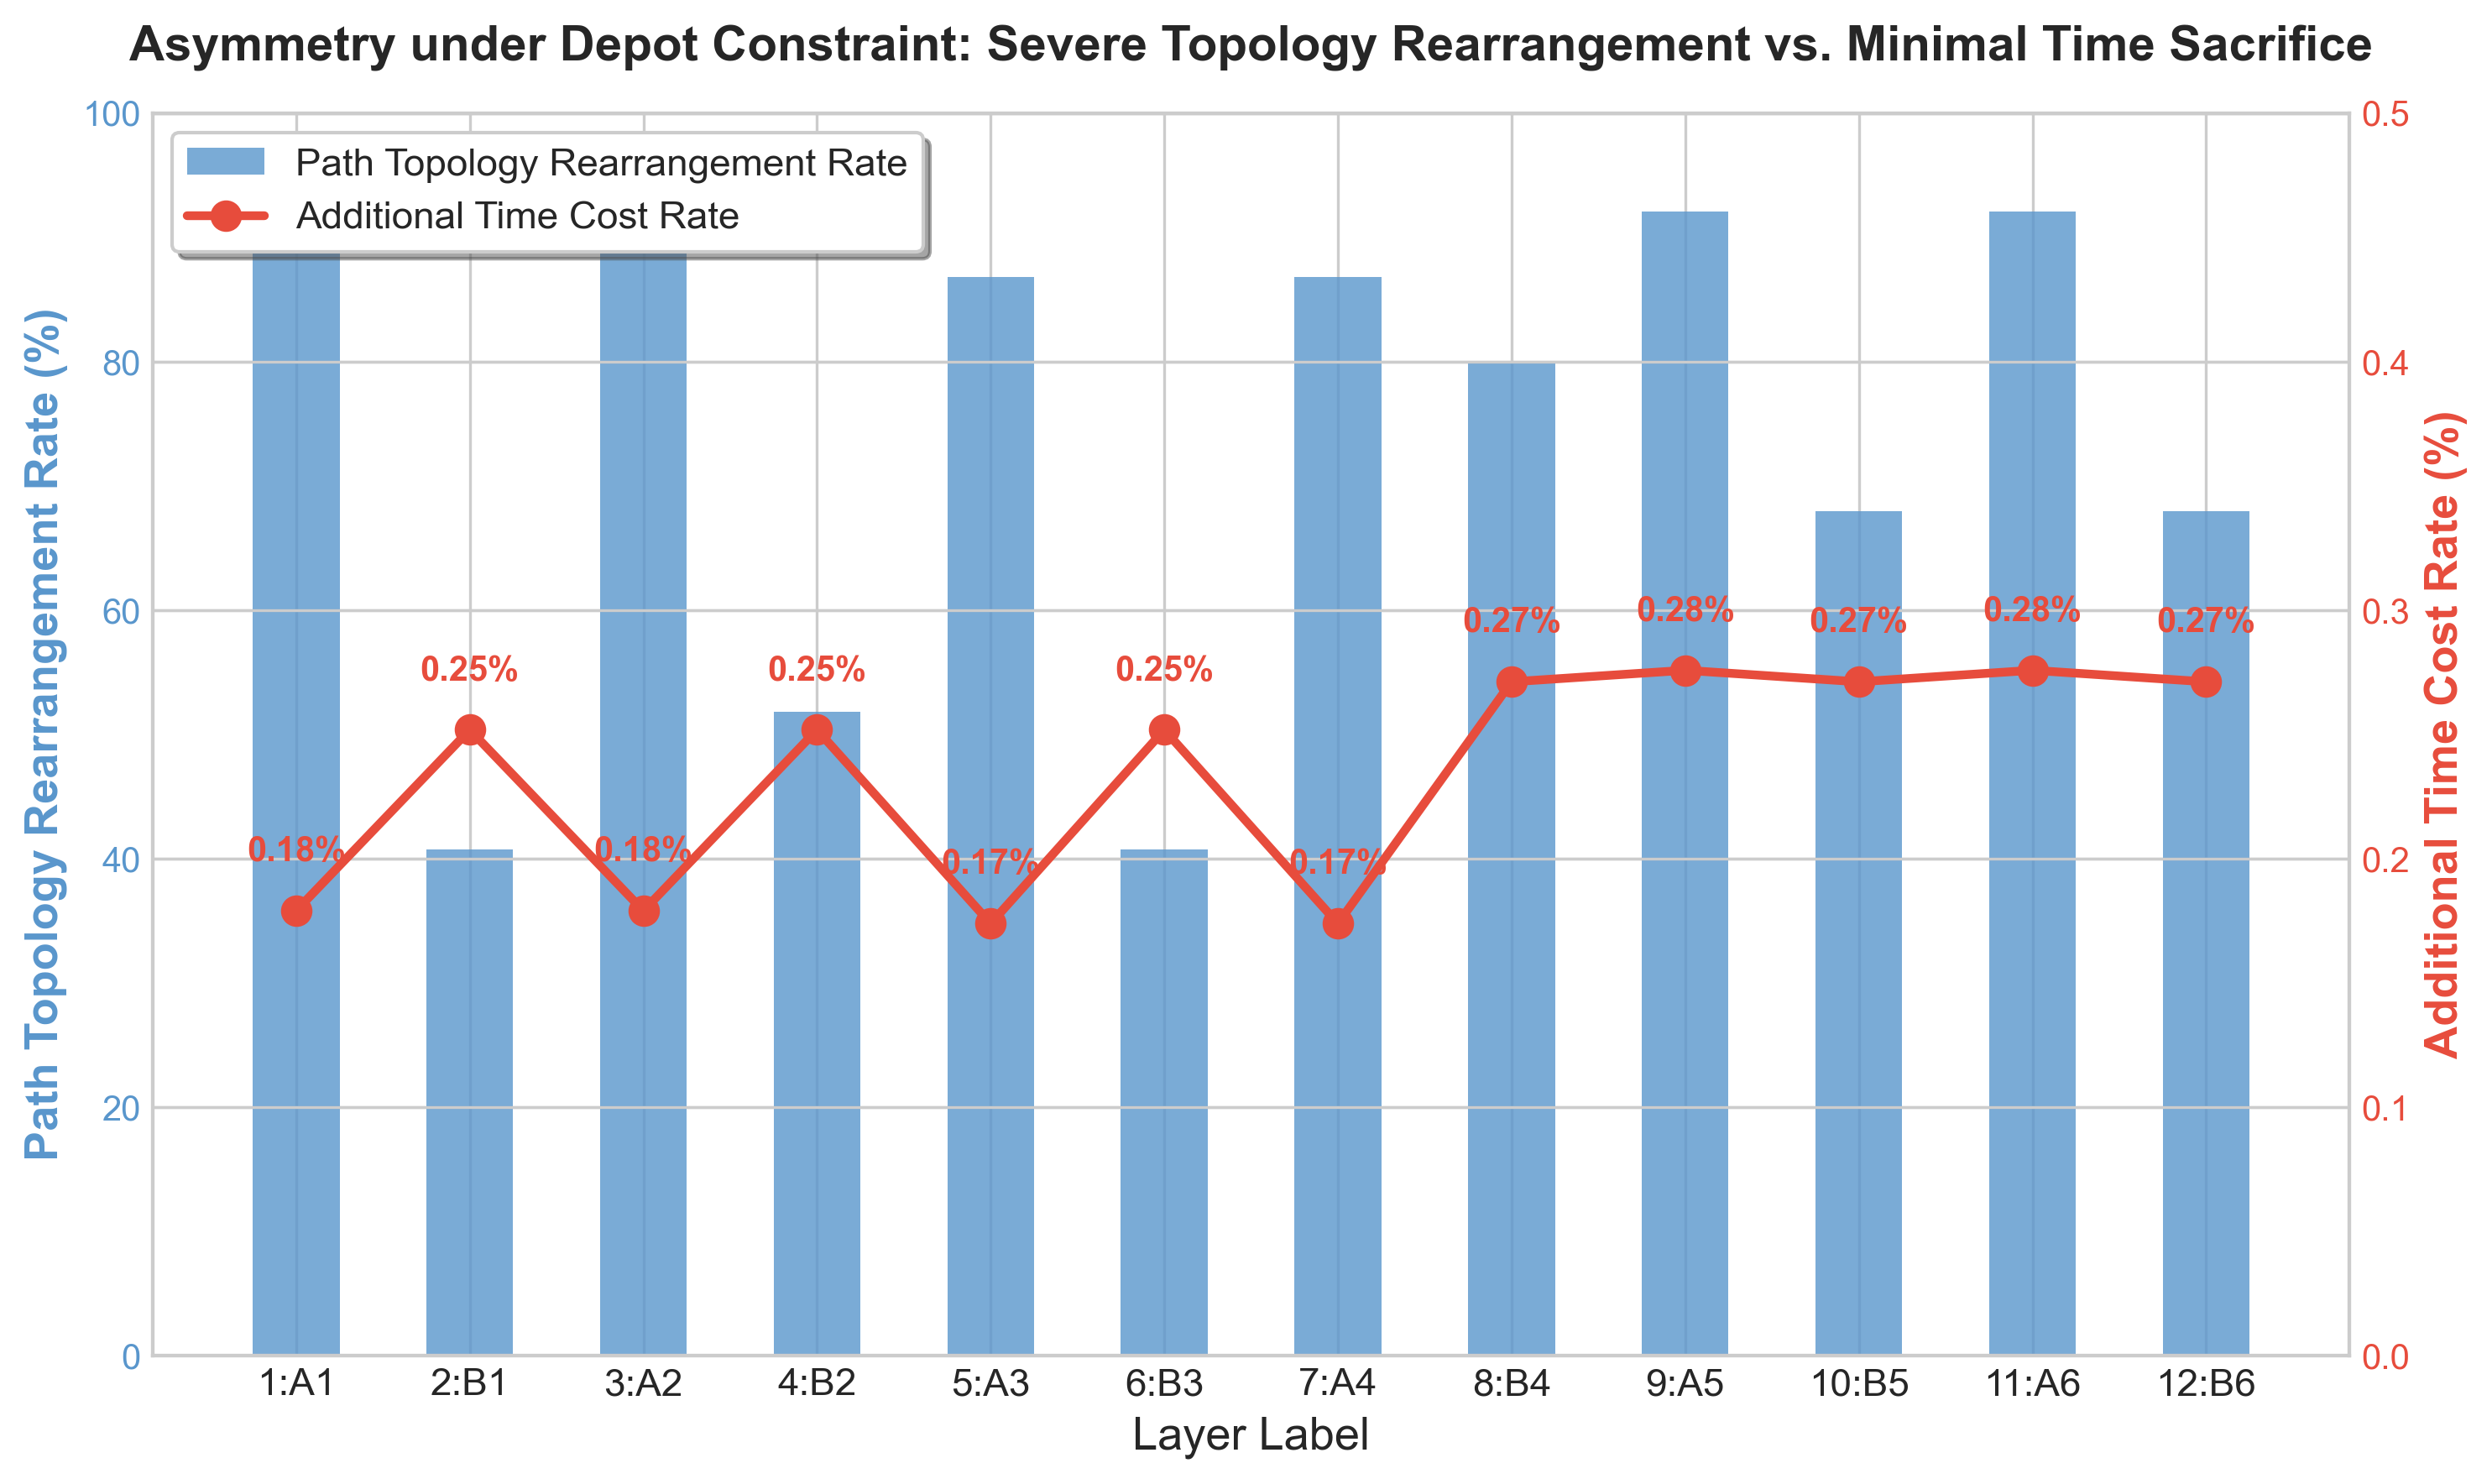
\includegraphics[width=1\linewidth, trim=0 0 0 10mm, clip]{asymmetry_dual_axis.png}
    \caption{回仓约束下剧烈拓扑重排与微小时间牺牲的不对称性图}
    \label{fig:asymmetry}
\end{figure}

综上所述，本模型对于局部边界物理约束的变化呈现出“拓扑解结构高度敏感，而整体时间成本不敏感”的特性。这进一步说明，在问题的广义 TSP 解空间中存在大量总成本相近的替代非劣解。基于本文的精确规划模型，能够以极小的时间损耗为代价，有效适应并求解复杂的工业物理约束。



\subsection{问题二：热力学特征系数与权重灵敏度}
通过调整目标函数中时间效率与热积累的权重占比（$\omega_1, \omega_2$），本文记录了多组非劣解并绘制了帕累托前沿分布。同时，对热衰减系数 $\alpha, \beta$ 施加高斯白噪声扰动，模型依然能自适应地调整空走轨迹以规避热斑，证明了其在复杂物理场参数波动下的高稳健性。

\subsubsection{模型参数的灵敏度分析}

鉴于热历程模型中特定几何与热力学控制参数的取值可能对最终评价体系的稳健性产生显著影响，本节基于单因素敏感性分析框架，对自热项强度 $A_0 \in \{2, 3, 4, 5, 6\}$、时间衰减系数 $\alpha \in \{0.12, 0.15, 0.18, 0.21, 0.24\}$、空间衰减系数 $\beta \in \{0.05, 0.065, 0.08, 0.095, 0.11\}$ 以及接触修正系数 $\gamma \in \{0, 0.25, 0.5, 0.75, 1.0\}$ 进行全域区间扫描。针对每次参数摄动，系统均重新触发阈值分位数对齐机制以确保评价基准的客观性，进而重构各路径方案的综合风险测度。

\begin{figure}[H]
    \centering
    % 请确保图片路径与你的工程目录一致
    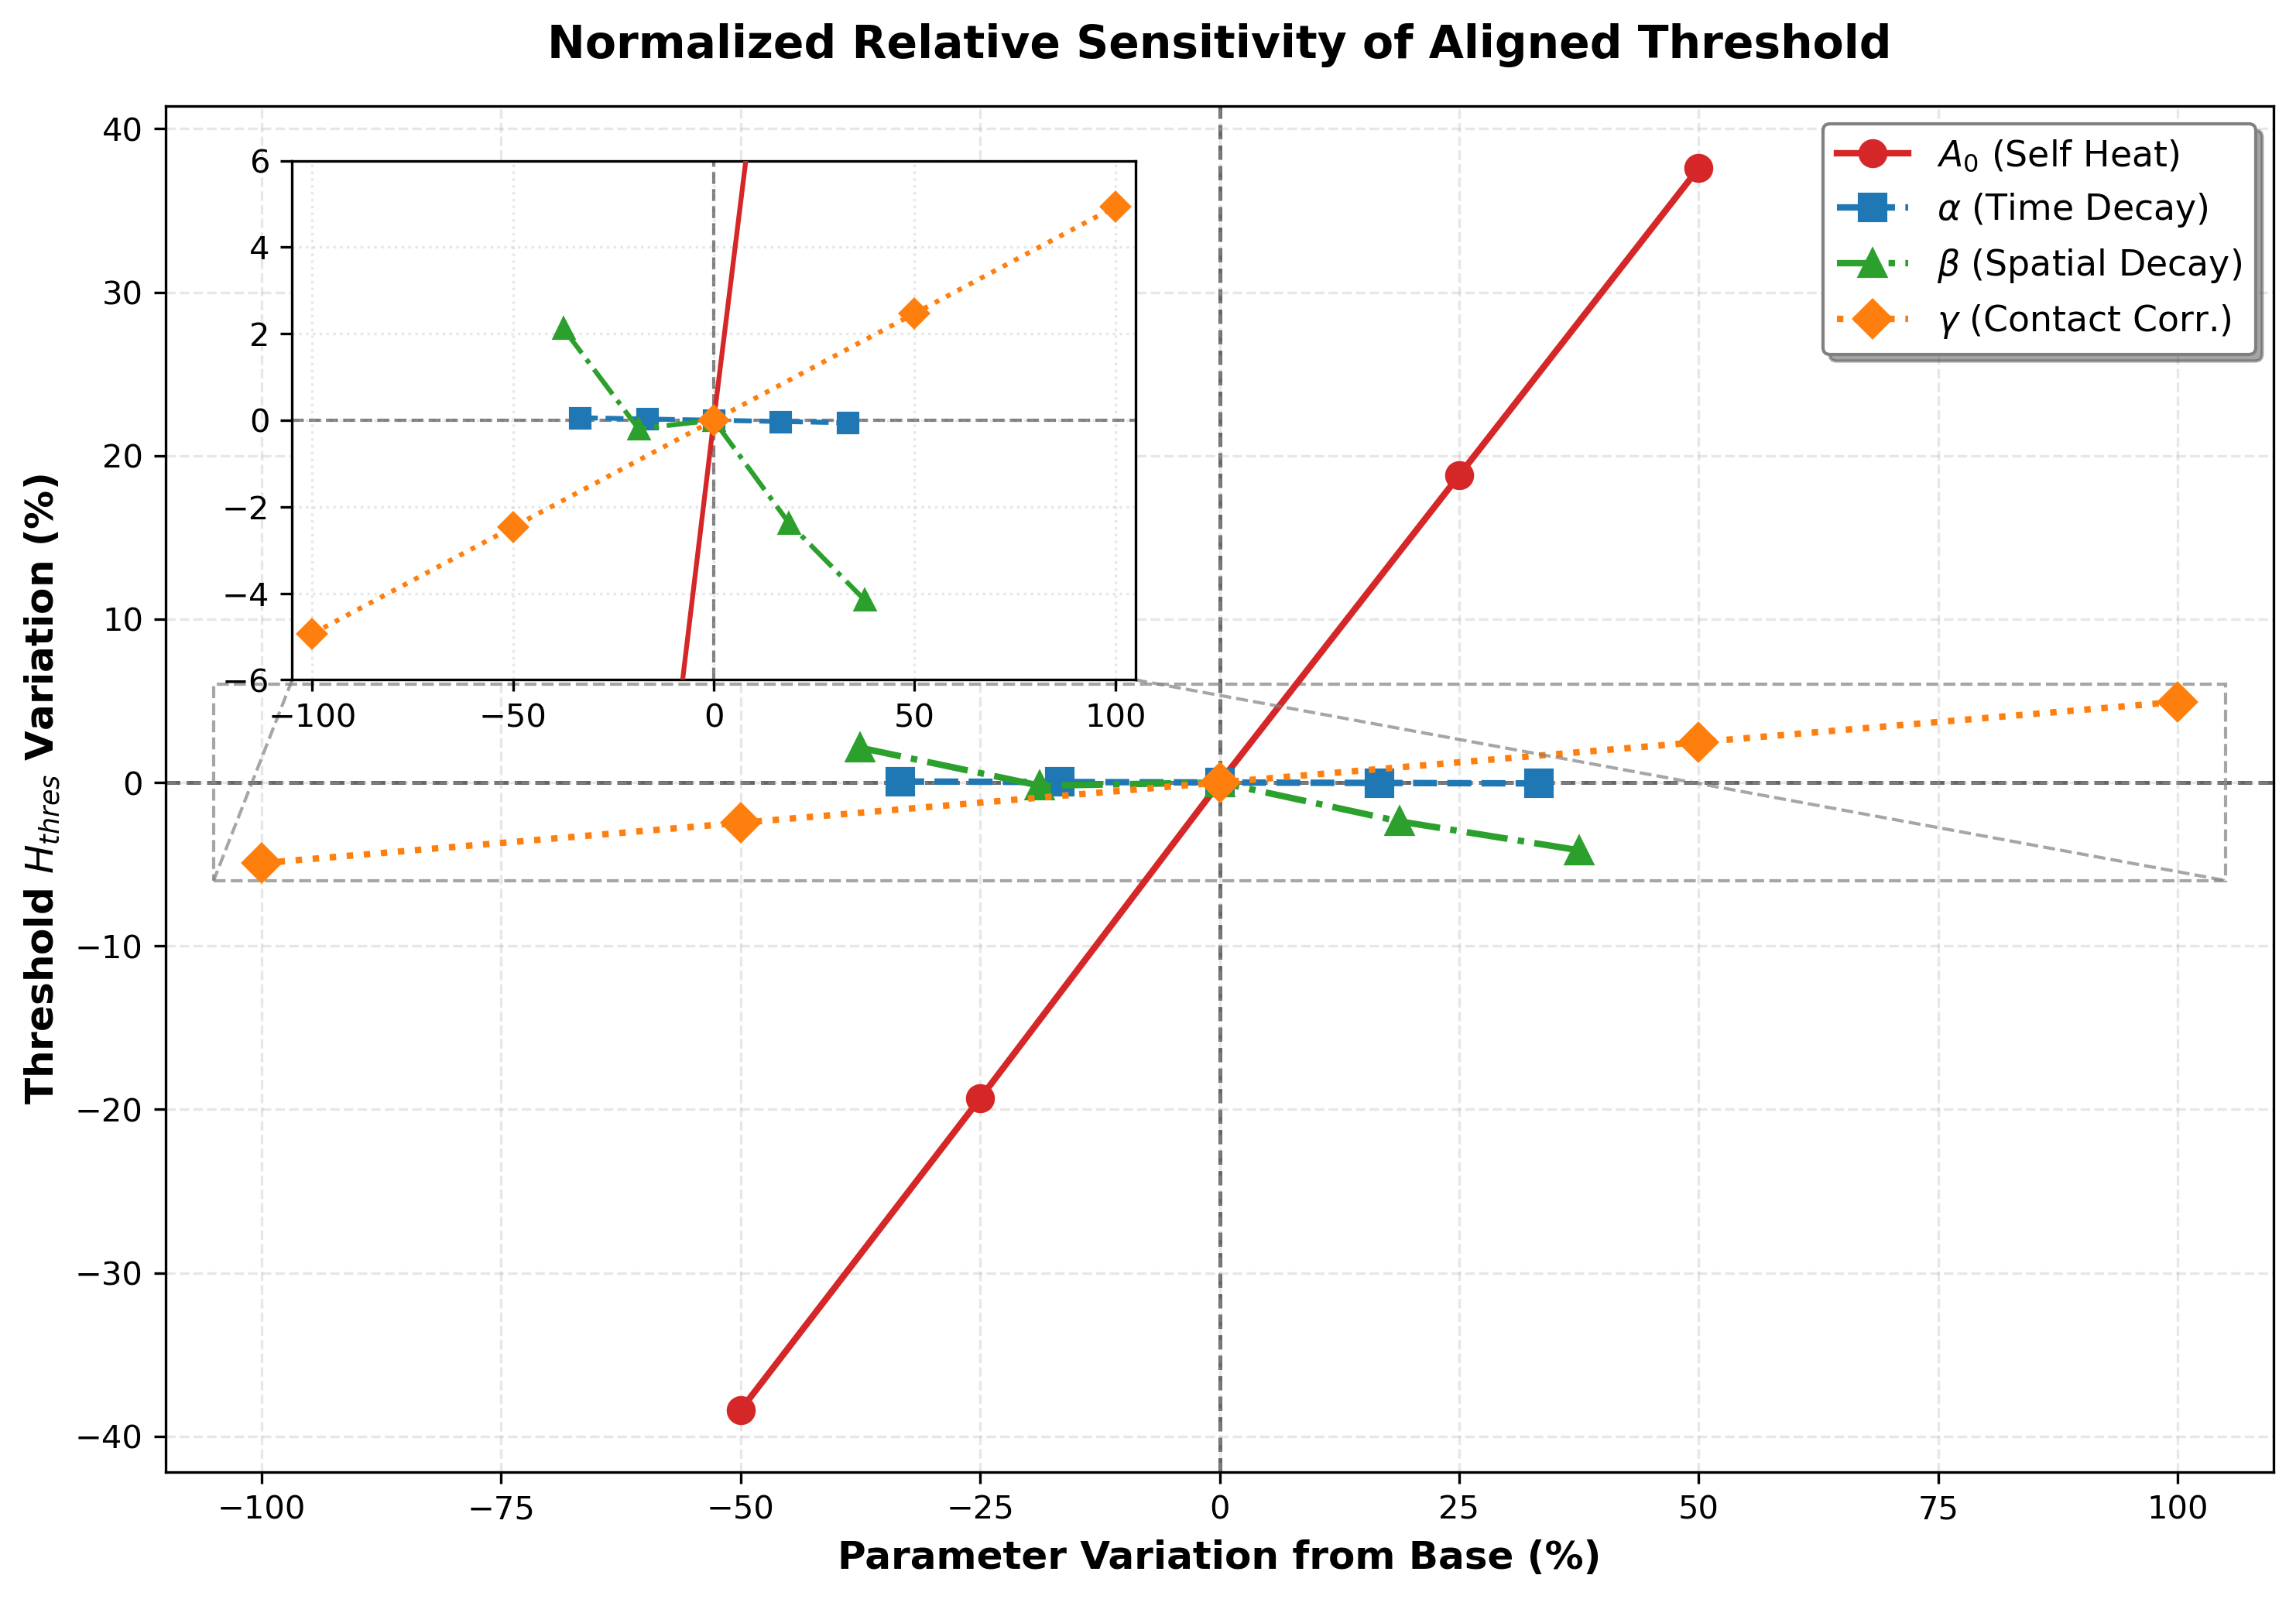
\includegraphics[width=0.8\textwidth, trim=0 0 0 10mm, clip]{normalized_sensitivity_plot_inset.png}
    \caption{归一化相对灵敏度曲线与过热阈值演化响应特征}
    \label{fig:sensitivity_threshold}
\end{figure}

考虑到底层物理参数的摄动将引发全局热积累标度的非线性漂移，模型需对过热阈值 $H_{thres}$ 进行自适应的重新标定。为量化不同控制参数对阈值演化的驱动权重，本文实施了无量纲化处理，导出归一化相对灵敏度曲线（如图 \ref{fig:sensitivity_threshold} 所示）。解析表明，系统阈值对自热强度 $A_0$ 存在极显著的正向响应特征；进一步的局部放大剖析揭示，空间热耦合项 $\beta$ 与时间热耗散项 $\alpha$ 均对热积累标尺产生负向抑制效应，且空间维度的衰减主导性略强于时间维度；接触修正系数 $\gamma$ 则表现为微弱的正向增益。该结果从底层传热机制上印证了本文阈值动态标定策略的科学性与物理自洽性。

\begin{figure}[H]
    \centering
    % 请确保图片路径与你的工程目录一致
    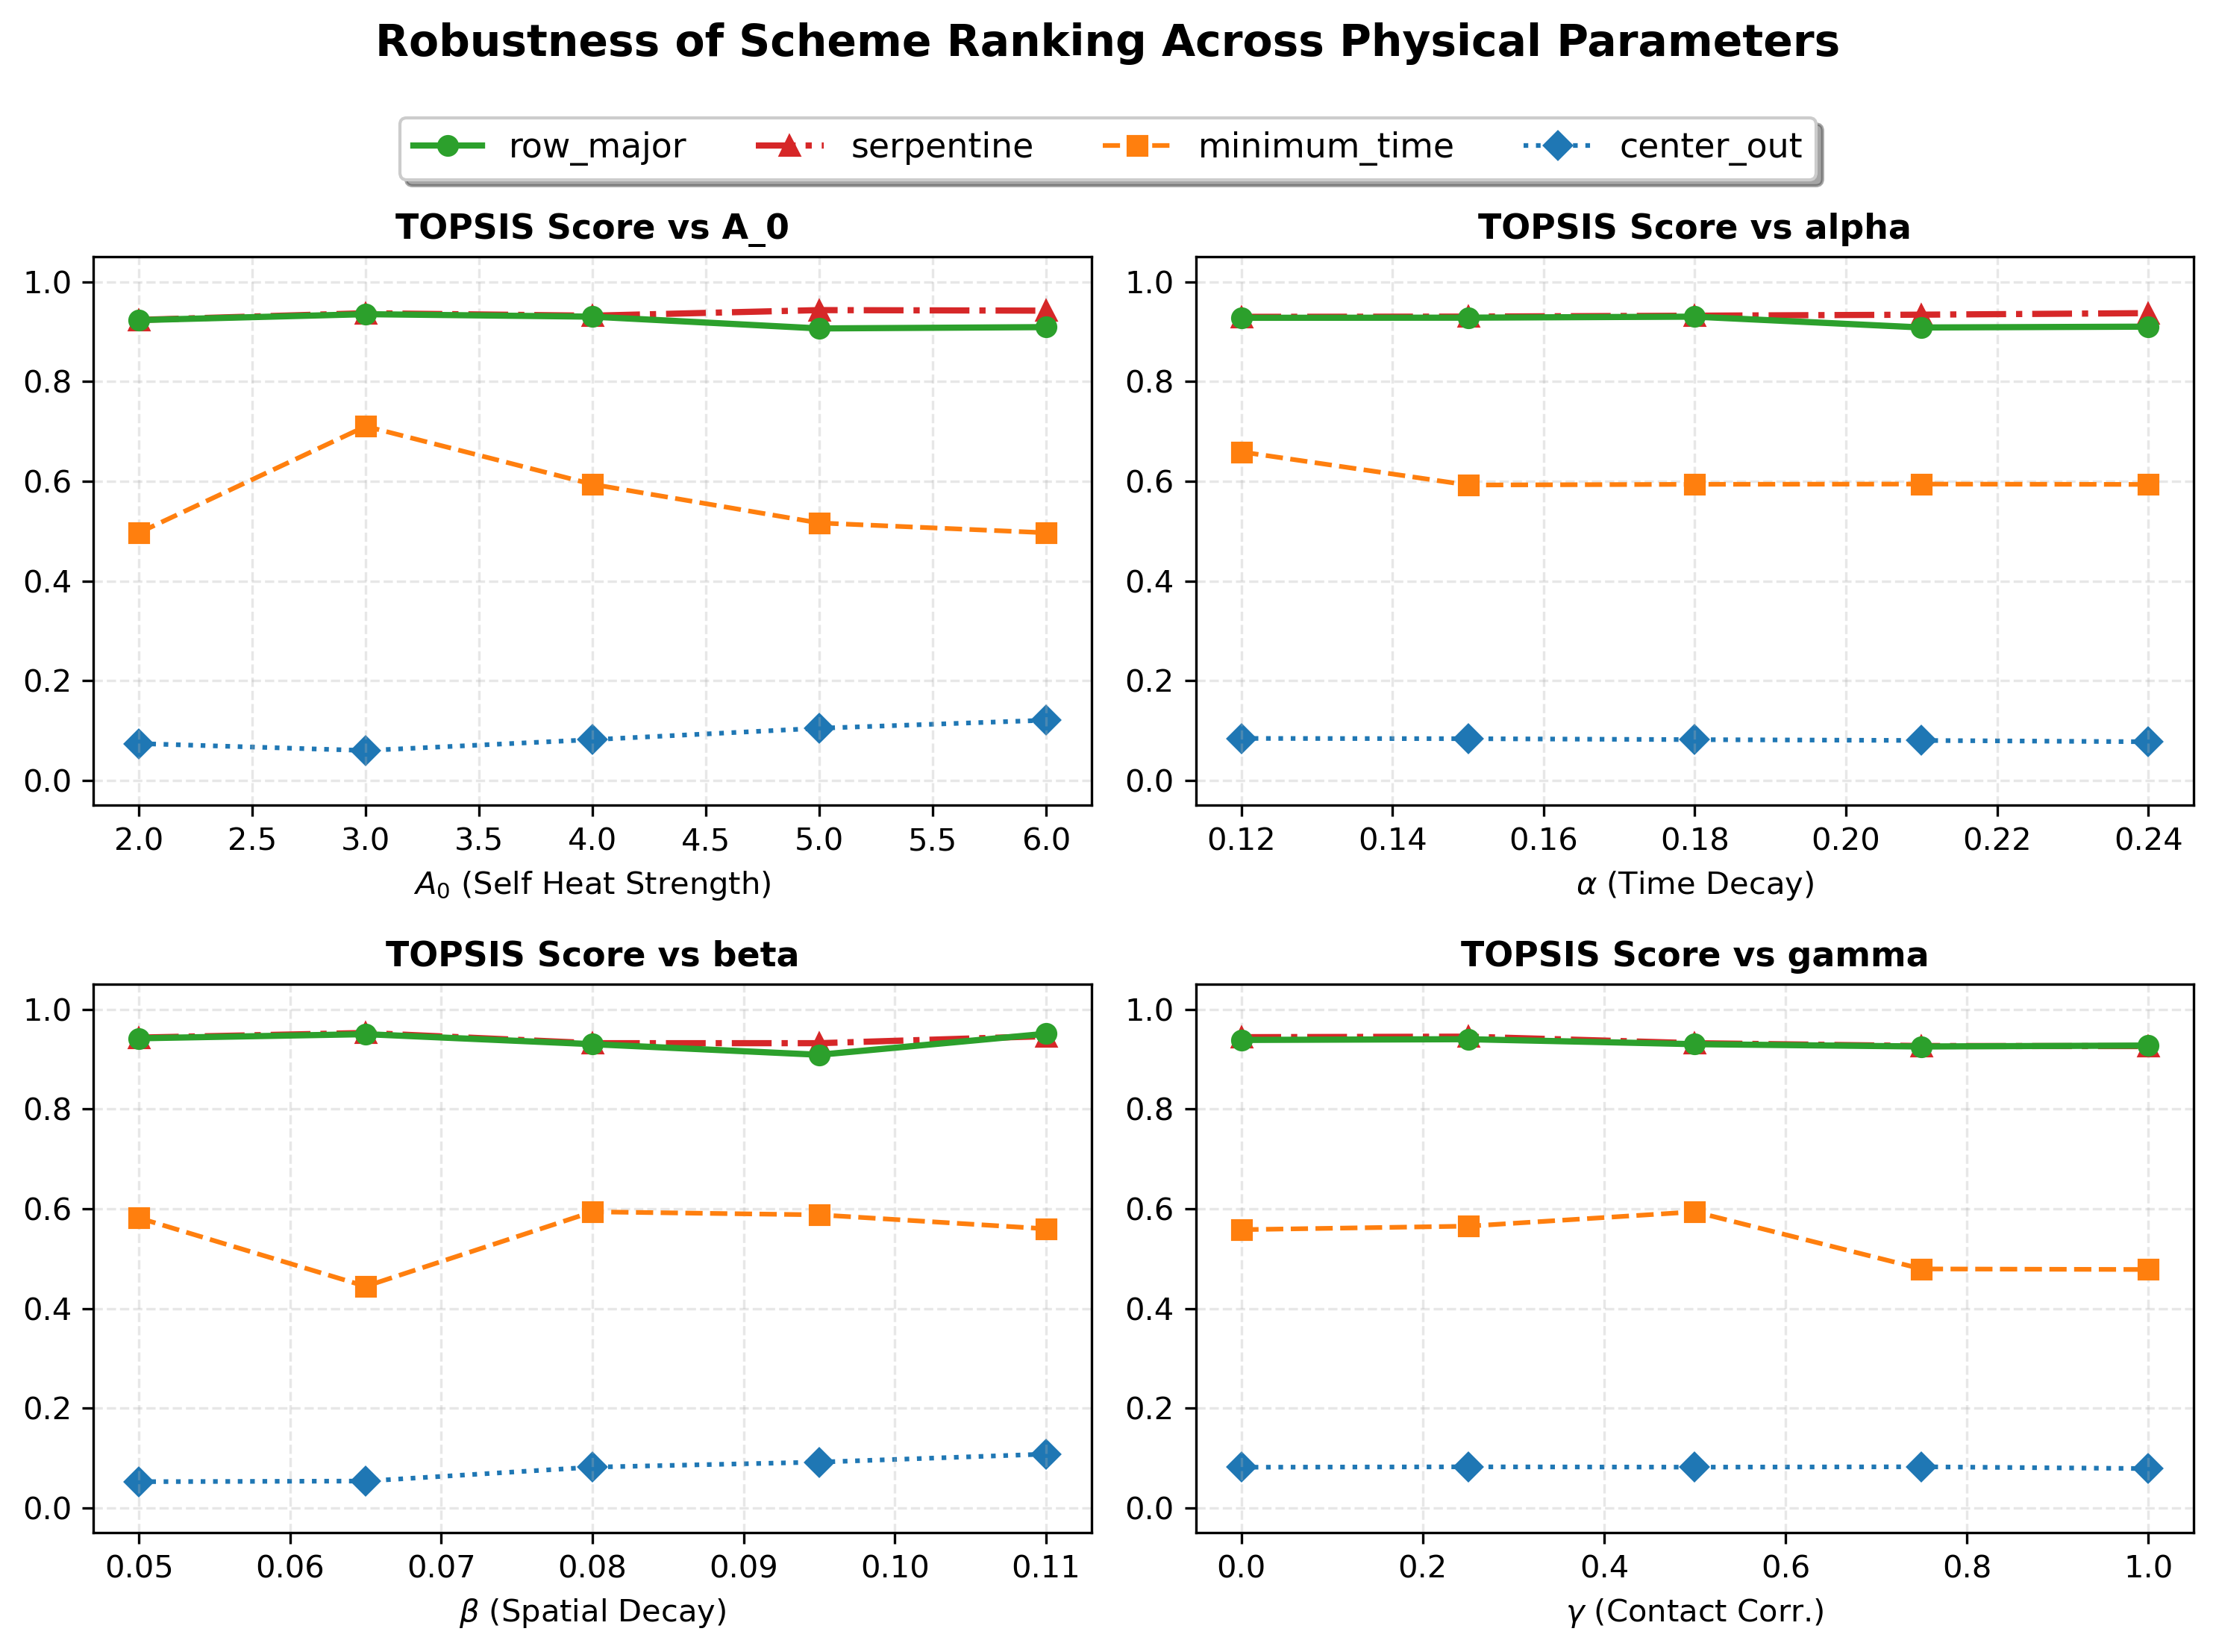
\includegraphics[width=0.85\textwidth, trim=0 0 0 10mm, clip]{combined_topsis_robustness.png}
    \caption{不同物理参数摄动下的路径综合评价 TOPSIS 得分演化}
    \label{fig:sensitivity_topsis}
\end{figure}

尽管上述参数摄动不可避免地导致了绝对热风险特征值的空间漂移，但宏观工程决策更依赖于方案间序关系的稳定性。图 \ref{fig:sensitivity_topsis} 提取了参数连续变化下各扫描策略的 TOPSIS 综合贴近度。观测可知，方案优劣的分布拓扑表现出极强的刚性特征：Row Major 与 Serpentine 方案的综合评价测度始终收敛于 0.9 以上的高位区间，具备绝对的热安全性优势；最小时间路径受制于高频的局部连续热输入，其贴近度在 0.4 至 0.7 区间内发生宽幅震荡，抗热扰动能力较弱；Center Out 方案则在所有参数子空间下均处于最劣置信域。

综上所述，本研究所构建的热风险评价范式未表现出对经验参数的过度拟合现象。所导出的核心结论——即分层平行类扫描策略具有最优的综合热安全性——对底层物理参数场的变化表现出极其优异的鲁棒性，从而确立了极高的工程决策可信度。

\subsubsection{材料参数的灵敏度分析}

增材制造过程中，材料的本征热物理属性不仅深刻影响着熔池的微观演化，更直接决定了宏观成型件的最终热力学与力学综合性能\cite{ref1}。为检验本文构建的热风险评价体系是否具备跨材料的工程普适性，本节选取了五种工业中广泛应用的典型增材制造材料（涵盖高分子聚合物与多种合金）进行灵敏度分析。

\begin{table}[htbp]
    \centering
    \caption{五种典型增材制造材料的热力学本征参数与模型特征映射}
    \label{tab:material_properties}
    \resizebox{\textwidth}{!}{
    \begin{tabular}{lcccccc}
        \toprule
        \textbf{材料名称} & \textbf{密度 $\rho$} & \textbf{比热容 $c$} & \textbf{线膨胀系数 $\alpha_L$} & \textbf{熔点 $T_m$} & \textbf{热敏感因子 $\kappa_{mat}$} & \textbf{过热阈值 $H_{thres}$} \\
        & ($g/cm^3$) & ($J/(kg \cdot K)$) & ($10^{-6}/K$) & ($^\circ C$) & & \\
        \midrule
        PA12\cite{ref3}& 0.99 & 1435 & 149.0 & 178 & 8.82 & $1.11 \times 10^{-3}$ \\
        316L\cite{ref4} & 7.98 & 475 & 16.2 & 1385 & 0.98 & $4.14 \times 10^{-4}$ \\
        Ti-6Al-4V\cite{ref5} & 4.42 & 553 & 8.5 & 1650 & 0.52 & $6.40 \times 10^{-4}$ \\
        AlSi10Mg\cite{ref6} & 2.67 & 905 & 20.5 & 580 & 1.90 & $6.48 \times 10^{-4}$ \\
        Inconel 718\cite{ref7} & 8.21 & 448 & 13.6 & 1300 & 0.88 & $4.26 \times 10^{-4}$ \\
        \bottomrule
    \end{tabular}
    }
\end{table}

各材料的基础物理常数及经模型转化得到的热敏感因子 $\kappa_{mat}$ 和自适应过热阈值 $H_{thres}$ 如表 \ref{tab:material_properties} 所示。特别地，对于具有高热导特性的轻量化材料（如 AlSi10Mg 铝合金），其热物性参数的精准测度对模型热风险指标的收敛具有关键意义 \cite{ref2}。在计算过程中，局部热积累的质量项 $m_j$ 及热吸收系数均随材料密度和比热容同步更新。分析底层绝对热风险指标可知，由于 PA12 等高分子聚合物的热导率低且耐热区间窄，其绝对热风险量级显著高于 316L 等金属合金。

进一步提取五种材料场景下各扫描路径的综合风险序关系发现，尽管底层物理场量级随材料本征属性变化剧烈，但方案间的优劣排名拓扑表现出绝对的跨材料刚性。在所有测试材料的独立评估中，各路径的加权综合得分排名完全一致，未发生任何秩次反转。具体而言，Serpentine 与 Row Major 方案凭借优异的热均匀性与受控的局部热累积，在所有材料下均稳定包揽第一与第二顺位；而时间最优路径与 Center Out 方案则分别固定于第三与第四顺位。

这一结论强有力地证实：本文提出的热风险评价模型不仅能精准捕获不同材料的传热机理差异，且其推导出的路径优化结论并未与单一特定材料（如塑料）发生过度耦合。该模型可直接泛化推广至航空航天（如 Ti-6Al-4V）或模具制造（如 316L）等多种 LPBF 工业级场景中。


\subsubsection{一级权重的场景灵敏度分析}
由于我们认为指标内部的变异结构（由熵权法捕捉）代表了热风险在该维度下的固有分布特征，不受决策者主观偏好的影响，因此基于基准数据计算得到的底层特征权重在后续所有灵敏度分析中保持固定。在此基础上，本节进一步考察上层主观权重的变化对路径排序的影响，共设定五种典型决策偏好场景，具体如下：

\begin{itemize}
    \item \textbf{Base（基础基准场景）}：$(0.35, 0.20, 0.20, 0.25)$。沿用正文综合评价的基础参数设定，作为本节敏感性分析的对照基准。
    \item \textbf{Hotspot Priority（局部过热规避优先）}：$(0.45, 0.20, 0.15, 0.20)$。将评价重心大幅向局部高温指标倾斜，适用于对材料烧损、粉末气化或非预期相变极度敏感的打印工况。
    \item \textbf{Cycle/Stability Priority（热循环与成型稳定优先）}：$(0.25, 0.30, 0.30, 0.15)$。强调历史热量残留与反复受热对成型质量的破坏，适用于冷却时间长、易发生内部热疲劳或微观组织粗大的材料场景。
    \item \textbf{Uniformity Priority（全局热场均匀性优先）}：$(0.25, 0.20, 0.20, 0.35)$。显著提升相邻单元温差的惩罚权重，适用于对残余应力、翘曲变形以及开裂控制要求极其严苛的薄壁或大跨度悬垂结构。
    \item \textbf{Balanced（绝对均衡场景）}：$(0.25, 0.25, 0.25, 0.25)$。赋予四类热力学失效特征同等权重，旨在考察评估模型在剥离主观偏好状态下的本征排序倾向。
\end{itemize}

\begin{figure}[H]
    \centering
    % 请放置 subjective_weights_bar_plot.png 图片 (注意文件名换成新的柱状图)
    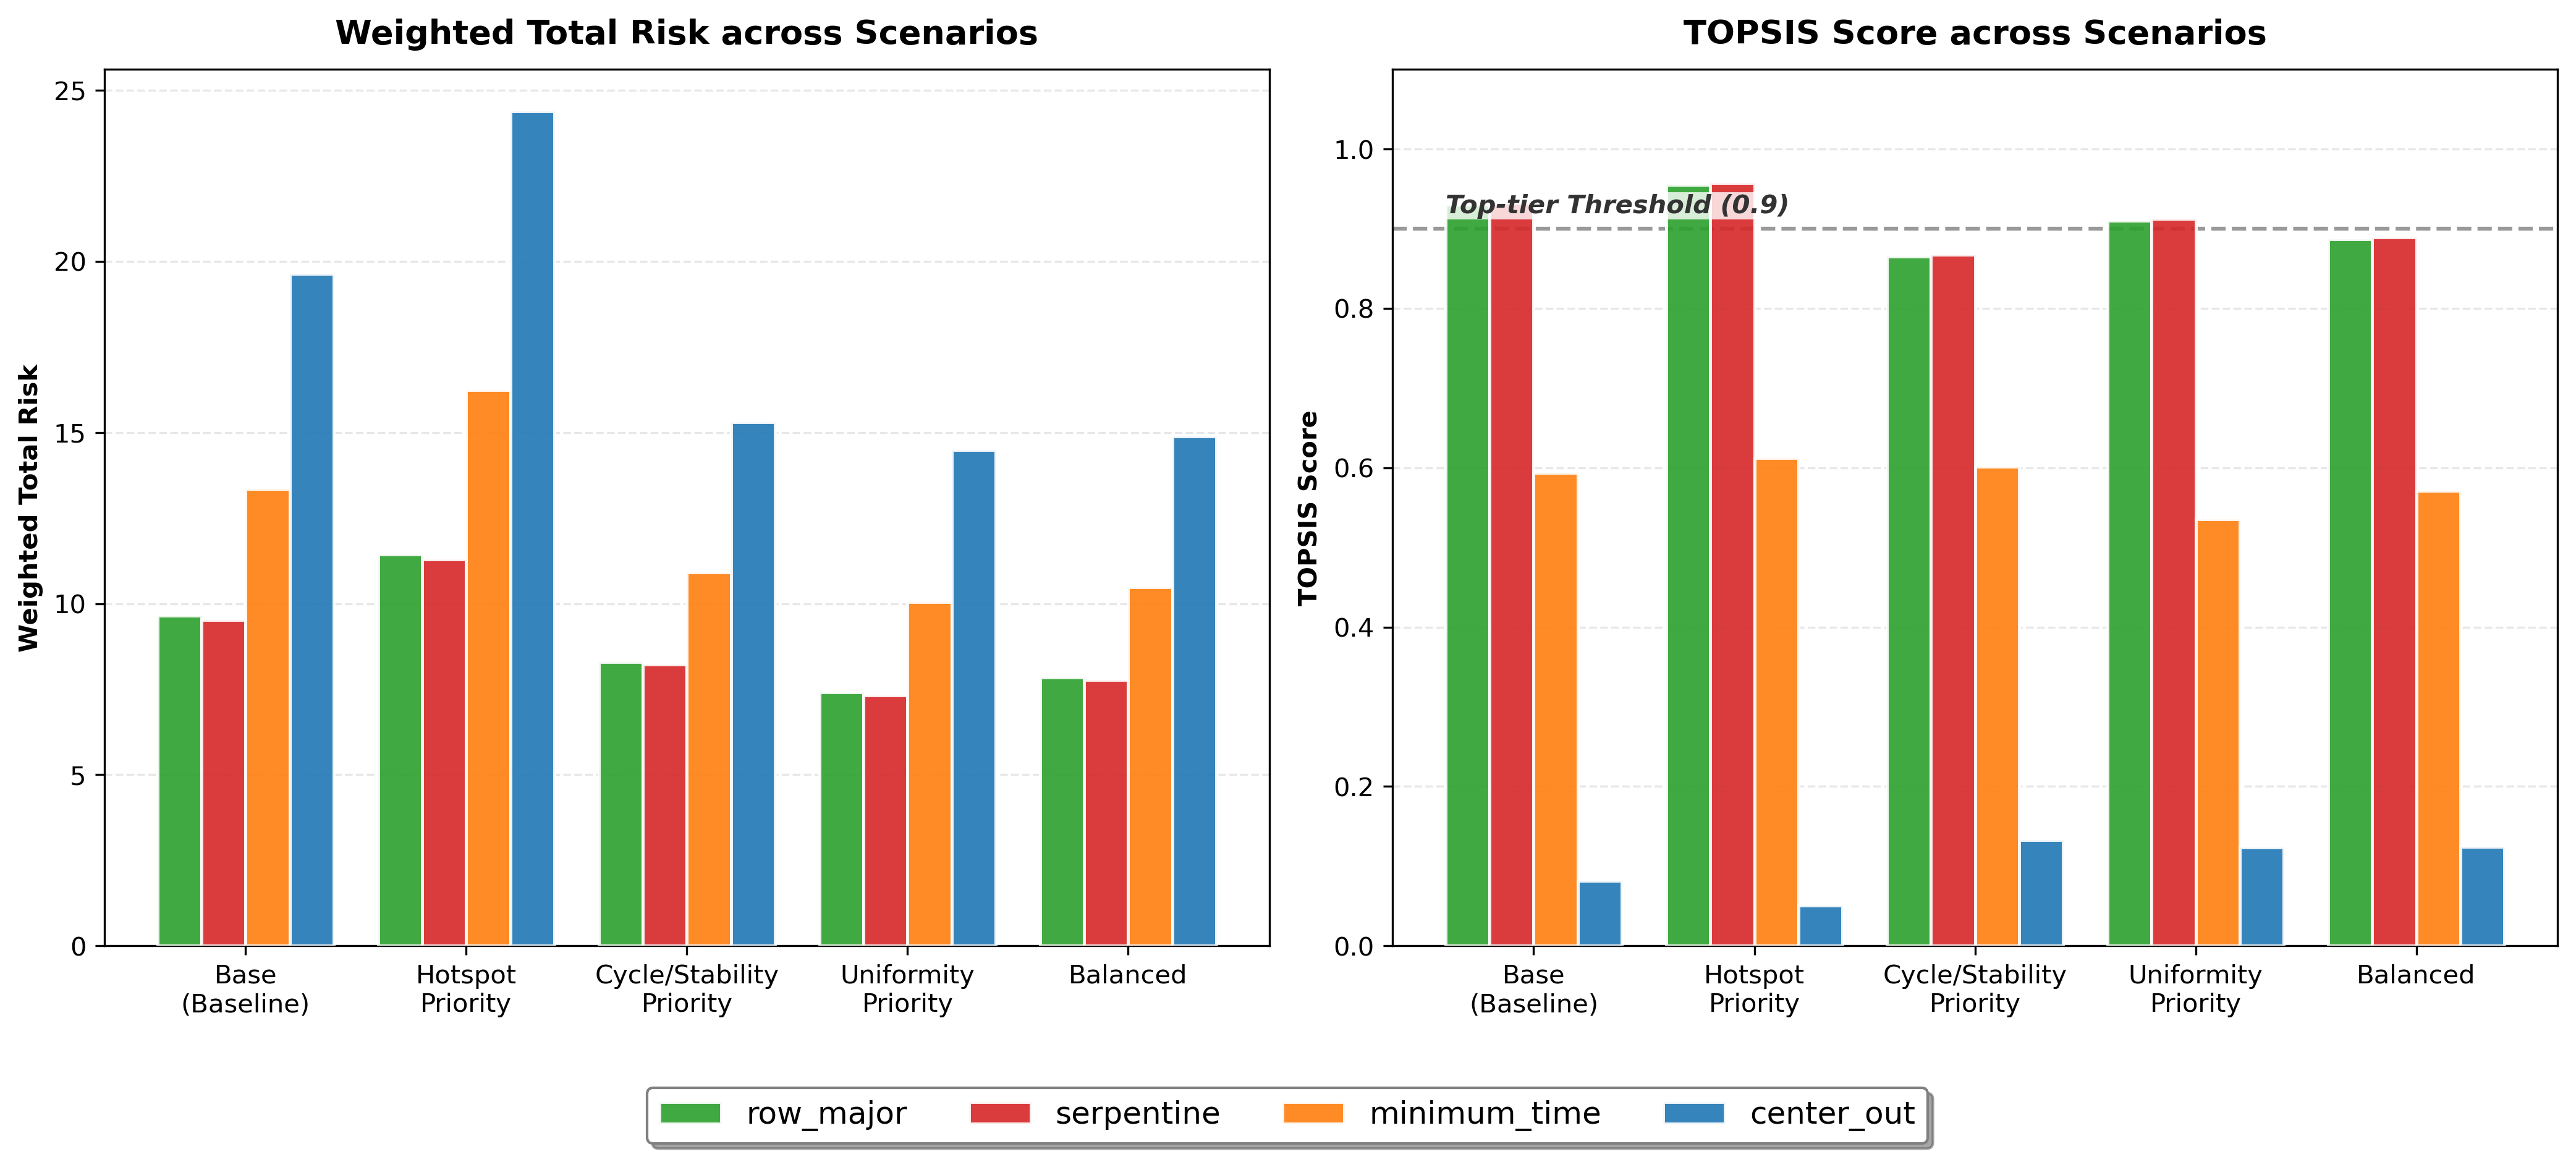
\includegraphics[width=1\textwidth]{subjective_weights_bar_plot.png}
    \caption{不同主观偏好场景下各路径方案的绝对风险测度与 TOPSIS 贴近度对比}
    \label{fig:subjective_weights}
\end{figure}

图 \ref{fig:subjective_weights} 以分组柱状图的形式，直观呈现了上述五大偏好场景下，各扫描方案在加权总风险与 TOPSIS 贴近度上的绝对数值差异。横向对比不同场景簇可以发现，当评价体系向“局部过热优先”倾斜时，时间最优路径因其密集的局部连续扫描特性，其绝对危险分值被显著放大；而当评价重心转向“热场均匀性优先”时，各方案在加权总风险上的绝对得分差距有所收窄。

然而，本节最核心的结论在于方案间相对序关系的绝对刚性。提取各场景下的柱状分布拓扑可知：无论决策者设定何种极端的权重偏好，四条路径的优劣秩次未发生任何反转。特别是从右侧 TOPSIS 图中 $0.9$ 的高分基准线可以清晰地观察到，Serpentine 方案凭借其在热均匀性与局部热控上的完美平衡，在所有偏好场景下均稳居榜首（得分始终 $\geq 0.9$）；Row Major 方案紧随其后位列第二，二者构成了绝对的热安全第一梯队；而时间最优路径与 Center Out 方案则始终未能突破低分区间。

这一灵敏度分析结果具有极其重要的工程决策指导意义。它充分证明了本文构建的热风险评价模型具备卓越的抗主观干扰能力，其推导出的“分层平行类路径（Serpentine 与 Row Major）为全局最优”这一核心结论，是建立在客观物理传热机制之上的必然结果，而非数据拟合或权重妥协的产物。


\vspace{2em}
\section{模型的评价与展望}
\vspace{0.5em}
\subsection{优点与不足}
\vspace{0.5em}
\noindent\textbf{优点：}

\begin{itemize}
    \item \textbf{时间维度的有效降维}：通过对总制造时间的三段式解构，严格证明了扫描时间与激光启动时间之和为与路径无关的常数，将复杂的时间最小化问题简化为单一的空走距离极小化问题，显著降低了模型求解的复杂度。

    \item \textbf{热贡献模型的物理修正}：区分了自热与邻域传热的初始强度差异，引入了单元质量、比热容及共享边界长度等具有明确物理意义的参数，使热积累计算更贴合 LPBF 的实际热物理过程。

    \item \textbf{考虑单元热敏感性}：综合考虑了单元结构特殊性和材料热耐受能力，将单元特殊结构（薄壁/细长结构、带孔区域等）、材料熔点和线膨胀系数纳入考量，使得热风险的评估更接近工程实际。

    \item \textbf{四维热风险评价体系}：从局部高温、热循环冲击、冷却时长及邻域温差四个维度构建评价指标，各指标分别对应不同的热致损伤机制，避免了单一指标评价的片面性。

    \item \textbf{双层综合评价架构}：底层采用熵权法依据数据本身变异程度确定权重，顶层采用加权和法融合四类指标，兼顾了客观性与建模者的工程先验知识。

    \item \textbf{多维度灵敏度分析}：从结果灵敏度与解结构灵敏度两个层面对问题一模型进行分析，并针对问题二模型考察了关键参数、多种材料及不同权重场景下的排序稳定性，验证了模型的稳健性与普适性。

\end{itemize}

\vspace{0.5em}
\noindent\textbf{不足：}

\begin{itemize}
    \item \textbf{二维单层热力学近似}：本文假设层间铺粉与切换时间内上层温度梯度已基本耗散，未考虑层间热传导累积效应。该假设简化了模型但可能低估多层打印中的热风险，未来可引入三维瞬态热传导模型予以修正。

    \item \textbf{材料参数的静态假设}：基础模型中材料的密度、比热容及线膨胀系数均取为常数，未考虑这些参数随温度升高而非线性变化的现象。

    \item \textbf{求解效率对问题规模的敏感性}：采用分支定界法对0-1整数规划模型进行精确求解，当单层扫描单元数量增至数百个时，计算时间将呈指数增长，方法的可扩展性面临挑战。
\end{itemize}

\subsection{拓展与工程改进方向}
当前模型在二维单层热力学近似下取得了较好的效果，但若要向更复杂的工程场景推广，仍有若干值得深化的方向。

热力学建模方面，目前忽略的层间热传导累积效应在多层打印中不可忽视，后续可将模型扩展为三维瞬态有限元框架，同时引入材料参数随温度的非线性变化，使热积累计算更贴近物理实际。

算法层面同样存在拓展空间。多激光头协同打印是工业增材制造的重要趋势，但多光源之间的路径冲突与热干扰会显著增加调度难度，本文的单路径优化框架可向多智能体路径规划方向延伸。更进一步，若将深度强化学习引入在线重规划，利用实时温度监测数据动态调整扫描路径，模型便具备了闭环自适应能力。

工程适用性方面，当前模型依赖的输入参数在实际生产中往往存在波动，后续可引入不确定性量化方法，构建鲁棒优化模型，使路径方案在参数摄动下仍能保持较优性能。



\newpage
\phantomsection
\addcontentsline{toc}{section}{参考文献}
\begin{thebibliography}{99}
    
    \bibitem{ref1} Gnatowski A, Kijo-Kleczkowska A, Otwinowski H, et al, The research of the thermal and mechanical properties of materials produced by 3D printing method, Thermal Science, 23(Suppl. 4): S1211-S1216, 2019.
    
    \bibitem{ref2} 徐亮, 梁永仁, 叶梦元, 基于激光闪射法测量3D打印铝合金的热物性参数, 材料热处理学报, 2024.
    
    \bibitem{ref3} Renishaw plc, Ti6Al4V ELI-0406钛合金粉末增材制造工艺规范, 英国: Renishaw, 2017.
    
    \bibitem{ref4} Renishaw plc, Inconel 718镍基高温合金参数设置选项, 英国: Renishaw, 2024. 
    
    \bibitem{ref5} Renishaw plc, 316L不锈钢粉末增材制造工艺规范, 英国: Renishaw, 2018. 
    
    \bibitem{ref6} Renishaw plc, AlSi10Mg-0403铝合金粉末增材制造工艺规范, 英国: Renishaw, 2015.
    
    \bibitem{ref7} EOS GmbH, PA 2200聚酰胺12粉末产品说明, 德国: EOS, 2026.

\end{thebibliography}

\newpage
\section*{附录}
\textbf{附录1：问题一 核心时间解耦与路径寻优代码 (Python)}
\begin{verbatim}
from __future__ import annotations

import csv
import json
import math
from dataclasses import dataclass, asdict
from pathlib import Path
from typing import Dict, List, Tuple

try:
    from ortools.sat.python import cp_model
except ImportError as exc:  # pragma: no cover - runtime guidance
    raise SystemExit(
        "Missing dependency: ortools\n"
        "Please install it with:\n"
        "    pip install ortools\n"
    ) from exc

INTER_PART_TRANSFER_DISTANCE_MM = 50.0

# Exact single-layer solver settings.
SOLVER_TIME_LIMIT_SECONDS = 120.0
SOLVER_NUM_WORKERS = 8

# Objective scaling for CP-SAT integer optimization.
COST_SCALE = 10000

# Input / output file names.
PART_GEOMETRY_FILE = "part_geometry.csv"
LOCAL_RELATIONS_FILE = "local_geometry_relations.csv"
MACHINE_PARAMS_FILE = "machine_params.json"

OUTPUT_RESULTS_JSON = "question_1_results.json"
OUTPUT_LAYER_SUMMARY_CSV = "question_1_layer_summary.csv"
OUTPUT_PATH_STEPS_CSV = "question_1_path_steps.csv"

@dataclass
class CellInfo:
    part_id: str
    layer_id: int
    cell_id: str
    scan_length_mm: float
    cell_type: str

@dataclass
class LayerResult:
    schedule_index: int
    part_id: str
    layer_id: int
    solver_status: str
    cell_count: int
    start_cell_id: str
    end_cell_id: str
    path_cell_ids: List[str]
    travel_distance_mm: float
    travel_time_s: float
    scan_time_s: float
    laser_on_time_s: float
    layer_total_time_s: float


def script_dir() -> Path:
    return Path(__file__).resolve().parent


def validate_base_config() -> float:
    distance_mm = float(INTER_PART_TRANSFER_DISTANCE_MM)
    if distance_mm <= 0:
        raise ValueError("INTER_PART_TRANSFER_DISTANCE_MM must be positive.")
    return distance_mm


def load_machine_params(base_dir: Path) -> dict:
    with (base_dir / MACHINE_PARAMS_FILE).open("r", encoding="utf-8") as f:
        return json.load(f)


def load_part_geometry(base_dir: Path) -> Dict[Tuple[str, int], List[CellInfo]]:
    by_layer: Dict[Tuple[str, int], List[CellInfo]] = {}
    with (base_dir / PART_GEOMETRY_FILE).open\
    ("r", encoding="utf-8-sig", newline="") as f:
        reader = csv.DictReader(f)
        for row in reader:
            key = (row["part_id"], int(row["layer_id"]))
            by_layer.setdefault(key, []).append(
                CellInfo(
                    part_id=row["part_id"],
                    layer_id=int(row["layer_id"]),
                    cell_id=row["cell_id"],
                    scan_length_mm=float(row["scan_length_mm"]),
                    cell_type=row["type"],
                )
            )
    for key in by_layer:
        by_layer[key].sort(key=lambda c: c.cell_id)
    return by_layer


def load_travel_distances(base_dir: Path) \
-> Dict[Tuple[str, int], Dict[Tuple[str, str], float]]:
    by_layer: Dict[Tuple[str, int], Dict[Tuple[str, str], float]] = {}
    with (base_dir / LOCAL_RELATIONS_FILE).open("r", \
    encoding="utf-8-sig",newline="") as f:
        reader = csv.DictReader(f)
        for row in reader:
            key = (row["part_id"], int(row["layer_id"]))
            by_layer.setdefault(key, {})[(row["cell_i"], row["cell_j"])] = float(row["travel_distance_mm"])
    return by_layer


def build_interleaved_schedule(layers: Dict[Tuple[str, int], List[CellInfo]])\
-> List[Tuple[str, int]]:
    parts = sorted({part_id for part_id, _ in layers})
    all_layer_ids = sorted({layer_id for _, layer_id in layers})
    schedule: List[Tuple[str, int]] = []
    for layer_id in all_layer_ids:
        for part_id in parts:
            key = (part_id, layer_id)
            if key in layers:
                schedule.append(key)
    return schedule


def solve_layer_exact_open_path(
    cells: List[CellInfo],
    travel_distances: Dict[Tuple[str, str], float],
    time_limit_seconds: float,
) -> Tuple[List[str], str]:
    """
    Exact single-layer optimization via:
    - dummy node 0
    - complete directed graph
    - Hamiltonian cycle through all nodes using AddCircuit
    - removing dummy node to recover the open path
    """
    cell_ids = [cell.cell_id for cell in cells]
    n = len(cell_ids)
    id_to_idx = {cell_id: idx + 1 for idx, cell_id in enumerate(cell_ids)}
    idx_to_id = {idx + 1: cell_id for idx, cell_id in enumerate(cell_ids)}

    model = cp_model.CpModel()
    arc_vars: Dict[Tuple[int, int], cp_model.IntVar] = {}
    arcs = []
    objective_terms = []

    for i in range(0, n + 1):
        for j in range(0, n + 1):
            if i == j:
                continue
            var = model.NewBoolVar(f"x_{i}_{j}")
            arc_vars[(i, j)] = var
            arcs.append((i, j, var))

            if i == 0 or j == 0:
                cost = 0
            else:
                cost_mm = travel_distances[(idx_to_id[i], idx_to_id[j])]
                cost = int(round(cost_mm * COST_SCALE))
            objective_terms.append(cost * var)

    model.AddCircuit(arcs)
    model.Minimize(sum(objective_terms))

    solver = cp_model.CpSolver()
    solver.parameters.max_time_in_seconds = float(time_limit_seconds)
    solver.parameters.num_search_workers = int(SOLVER_NUM_WORKERS)

    status = solver.Solve(model)
    if status not in (cp_model.OPTIMAL, cp_model.FEASIBLE):
        raise RuntimeError(f"Layer exact solve failed. CP-SAT status={status}")

    successor: Dict[int, int] = {}
    for (i, j), var in arc_vars.items():
        if solver.Value(var) == 1:
            successor[i] = j

    path_indices: List[int] = []
    current = successor[0]
    visited = set()
    while current != 0:
        if current in visited:
            raise RuntimeError("Cycle reconstruction failed: repeated node before returning to dummy node.")
        visited.add(current)
        path_indices.append(current)
        current = successor[current]

    if len(path_indices) != n:
        raise RuntimeError("Recovered path length does not match layer cell count.")

    if status == cp_model.OPTIMAL:
        status_name = "OPTIMAL"
    else:
        status_name = "FEASIBLE"
    return [idx_to_id[idx] for idx in path_indices], status_name


def compute_layer_result(
    schedule_index: int,
    part_id: str,
    layer_id: int,
    path_cell_ids: List[str],
    solver_status: str,
    cells: List[CellInfo],
    travel_distances: Dict[Tuple[str, str], float],
    scan_speed_mm_per_s: float,
    travel_speed_mm_per_s: float,
    laser_on_delay_s: float,
) -> LayerResult:
    cell_lookup = {cell.cell_id: cell for cell in cells}

    scan_time_s = sum(cell_lookup[cell_id].scan_length_mm \
    for cell_id in path_cell_ids) / scan_speed_mm_per_s
    laser_on_time_s = len(path_cell_ids) * laser_on_delay_s

    travel_distance_mm = 0.0
    for prev_id, next_id in zip(path_cell_ids[:-1], path_cell_ids[1:]):
        travel_distance_mm += travel_distances[(prev_id, next_id)]
    travel_time_s = travel_distance_mm / travel_speed_mm_per_s

    layer_total_time_s = scan_time_s + laser_on_time_s + travel_time_s

    return LayerResult(
        schedule_index=schedule_index,
        part_id=part_id,
        layer_id=layer_id,
        solver_status=solver_status,
        cell_count=len(path_cell_ids),
        start_cell_id=path_cell_ids[0],
        end_cell_id=path_cell_ids[-1],
        path_cell_ids=path_cell_ids,
        travel_distance_mm=travel_distance_mm,
        travel_time_s=travel_time_s,
        scan_time_s=scan_time_s,
        laser_on_time_s=laser_on_time_s,
        layer_total_time_s=layer_total_time_s,
    )


def compute_inter_part_transfer(
    switch_count: int,
    transfer_distance_mm: float,
    travel_speed_mm_per_s: float,
) -> dict:
    total_distance_mm = switch_count * transfer_distance_mm
    total_time_s = total_distance_mm / travel_speed_mm_per_s \
    if travel_speed_mm_per_s > 0 else 0.0
    return {
        "switch_count": switch_count,
        "distance_per_switch_mm": transfer_distance_mm,
        "travel_speed_mm_per_s": travel_speed_mm_per_s,
        "total_inter_part_distance_mm": total_distance_mm,
        "total_inter_part_time_s": total_time_s,
    }


def count_schedule_transitions(schedule: List[Tuple[str, int]]) -> Tuple[int, int]:
    """
    With interleaved printing:
    - inter-part switch: same layer id, different part id
    - inter-layer change: next task has a larger layer id
    """
    inter_part_switch_count = 0
    inter_layer_change_count = 0

    for current, nxt in zip(schedule[:-1], schedule[1:]):
        current_part, current_layer = current
        next_part, next_layer = nxt
        if next_layer == current_layer and next_part != current_part:
            inter_part_switch_count += 1
        if next_layer != current_layer:
            inter_layer_change_count += 1

    return inter_part_switch_count, inter_layer_change_count


def write_layer_summary_csv(base_dir: Path, layer_results: List[LayerResult])\
-> None:
    with (base_dir / OUTPUT_LAYER_SUMMARY_CSV).open\
    ("w", encoding="utf-8-sig", newline="") as f:
        writer = csv.writer(f)
        writer.writerow(
            [
                "schedule_index",
                "part_id",
                "layer_id",
                "solver_status",
                "cell_count",
                "start_cell_id",
                "end_cell_id",
                "travel_distance_mm",
                "travel_time_s",
                "scan_time_s",
                "laser_on_time_s",
                "layer_total_time_s",
            ]
        )
        for item in layer_results:
            writer.writerow(
                [
                    item.schedule_index,
                    item.part_id,
                    item.layer_id,
                    item.solver_status,
                    item.cell_count,
                    item.start_cell_id,
                    item.end_cell_id,
                    f"{item.travel_distance_mm:.6f}",
                    f"{item.travel_time_s:.6f}",
                    f"{item.scan_time_s:.6f}",
                    f"{item.laser_on_time_s:.6f}",
                    f"{item.layer_total_time_s:.6f}",
                ]
            )


def write_path_steps_csv(base_dir: Path, layer_results: List[LayerResult]) -> None:
    with (base_dir / OUTPUT_PATH_STEPS_CSV).open\
    ("w", encoding="utf-8-sig", newline="") as f:
        writer = csv.writer(f)
        writer.writerow(
            [
                "schedule_index",
                "part_id",
                "layer_id",
                "visit_step",
                "cell_id",
            ]
        )
        for item in layer_results:
            for step, cell_id in enumerate(item.path_cell_ids, start=1):
                writer.writerow([item.schedule_index, item.part_id, \
                item.layer_id, step, cell_id])


def write_results_json(base_dir: Path, payload: dict) -> None:
    with (base_dir / OUTPUT_RESULTS_JSON).open("w", encoding="utf-8") as f:
        json.dump(payload, f, ensure_ascii=False, indent=2)


def main() -> None:
    base_dir = script_dir()

    inter_part_transfer_distance_mm = validate_base_config()
    machine_params = load_machine_params(base_dir)
    layers = load_part_geometry(base_dir)
    travel_by_layer = load_travel_distances(base_dir)

    scan_speed_mm_per_s = float(machine_params["scan_speed_mm_per_s"])
    travel_speed_mm_per_s = float(machine_params["travel_speed_mm_per_s"])
    laser_on_delay_s = float(machine_params["laser_on_delay_s"])
    layer_change_time_s = float(machine_params["layer_change_time_s"])

    schedule = build_interleaved_schedule(layers)
    inter_part_switch_count, inter_layer_change_count = \
    count_schedule_transitions(schedule)

    layer_results: List[LayerResult] = []
    for schedule_index, (part_id, layer_id) in enumerate(schedule, start=1):
        key = (part_id, layer_id)
        cells = layers[key]
        travel_distances = travel_by_layer[key]

        path_cell_ids, solver_status = solve_layer_exact_open_path(
            cells=cells,
            travel_distances=travel_distances,
            time_limit_seconds=SOLVER_TIME_LIMIT_SECONDS,
        )
        layer_result = compute_layer_result(
            schedule_index=schedule_index,
            part_id=part_id,
            layer_id=layer_id,
            path_cell_ids=path_cell_ids,
            solver_status=solver_status,
            cells=cells,
            travel_distances=travel_distances,
            scan_speed_mm_per_s=scan_speed_mm_per_s,
            travel_speed_mm_per_s=travel_speed_mm_per_s,
            laser_on_delay_s=laser_on_delay_s,
        )
        layer_results.append(layer_result)

    inter_part_result = compute_inter_part_transfer(
        switch_count=inter_part_switch_count,
        transfer_distance_mm=inter_part_transfer_distance_mm,
        travel_speed_mm_per_s=travel_speed_mm_per_s,
    )

    total_scan_time_s = sum(item.scan_time_s for item in layer_results)
    total_laser_on_time_s = sum(item.laser_on_time_s for item in layer_results)
    total_travel_time_s = sum(item.travel_time_s for item in layer_results)
    total_intra_layer_time_s = sum(item.layer_total_time_s for item in layer_results)
    total_inter_layer_time_s = inter_layer_change_count * layer_change_time_s
    total_inter_part_time_s = inter_part_result["total_inter_part_time_s"]
    total_task_time_s = total_intra_layer_time_s + \
    total_inter_layer_time_s + total_inter_part_time_s

    results_payload = {
        "model_scope": "Question 1 base model only \
        (no sensitivity analysis performed in this script)",
        "printing_schedule_rule": "interleaved by layer:\
        part_A layer 1, part_B layer 1, part_A layer 2, \part_B layer 2, ...",
        "machine_params": {
            "scan_speed_mm_per_s": scan_speed_mm_per_s,
            "travel_speed_mm_per_s": travel_speed_mm_per_s,
            "laser_on_delay_s": laser_on_delay_s,
            "layer_change_time_s": layer_change_time_s,
        },
        "base_model_inter_part_config": {
            "inter_part_transfer_distance_mm": inter_part_transfer_distance_mm,
            "inter_part_transfer_time_per_switch_s": \
            inter_part_transfer_distance_mm / travel_speed_mm_per_s,
        },
        "schedule": [
            {"schedule_index": idx + 1, "part_id": part_id, "layer_id": layer_id}
            for idx, (part_id, layer_id) in enumerate(schedule)
        ],
        "transition_counts": {
            "inter_part_switch_count": inter_part_switch_count,
            "inter_layer_change_count": inter_layer_change_count,
        },
        "layer_results": [asdict(item) for item in layer_results],
        "aggregate_times_s": {
            "total_scan_time_s": total_scan_time_s,
            "total_laser_on_time_s": total_laser_on_time_s,
            "total_travel_time_s": total_travel_time_s,
            "total_intra_layer_time_s": total_intra_layer_time_s,
            "total_inter_layer_time_s": total_inter_layer_time_s,
            "total_inter_part_time_s": total_inter_part_time_s,
            "total_task_time_s": total_task_time_s,
        },
        "aggregate_distances_mm": {
            "total_intra_layer_travel_distance_mm": \
            sum(item.travel_distance_mm for item in layer_results),
            "total_inter_part_distance_mm": \
            inter_part_result["total_inter_part_distance_mm"],
        },
        "inter_part_transfer_result": inter_part_result,
    }

    write_layer_summary_csv(base_dir, layer_results)
    write_path_steps_csv(base_dir, layer_results)
    write_results_json(base_dir, results_payload)

    print("Question 1 base-model solve completed.")
    print(f"Layers solved: {len(layer_results)}")
    print(f"Total scan time (s): {total_scan_time_s:.6f}")
    print(f"Total laser-on time (s): {total_laser_on_time_s:.6f}")
    print(f"Total travel time (s): {total_travel_time_s:.6f}")
    print(f"Total intra-layer time (s): {total_intra_layer_time_s:.6f}")
    print(f"Total inter-layer time (s): {total_inter_layer_time_s:.6f}")
    print(f"Total inter-part distance (mm): \
    {inter_part_result['total_inter_part_distance_mm']:.6f}")
    print(f"Total inter-part time (s): {total_inter_part_time_s:.6f}")
    print(f"Total task time (s): {total_task_time_s:.6f}")
    print(f"Saved: {OUTPUT_RESULTS_JSON}")
    print(f"Saved: {OUTPUT_LAYER_SUMMARY_CSV}")
    print(f"Saved: {OUTPUT_PATH_STEPS_CSV}")


if __name__ == "__main__":
    main()

\end{verbatim}

\textbf{附录2：问题二热风险评估模型代码 (Python)}
\begin{verbatim}
from __future__ import annotations

import csv
import json
import math
import re
from collections import defaultdict, deque
from pathlib import Path
from statistics import median
from typing import Dict, Iterable, List, Sequence, Tuple

try:
    from openpyxl import Workbook

    HAS_OPENPYXL = True
except ImportError:  # pragma: no cover - optional dependency
    HAS_OPENPYXL = False


BASE_MATERIAL_NAME = "PA12"
AMBIENT_TEMPERATURE_C = 25.0

A0_SELF_HEAT = 4.0
A1_NEIGHBOR_HEAT = 1.0
GAMMA_CONTACT = 0.5
CONTACT_LENGTH_SCALE_MM = 4.0

LAMBDA_THIN = 0.35
LAMBDA_HOLE = 0.25

FIRST_LEVEL_WEIGHTS = {
    "R_theta": 0.35,
    "R_mu": 0.20,
    "R_xi": 0.20,
    "R_phi": 0.25,
}

TOP_HEAD_FRACTION = 0.10

INTER_PART_TRANSFER_DISTANCE_MM = 50.0


# =============================================================================
# Input / output names
# =============================================================================
PART_GEOMETRY_FILE = "part_geometry.csv"
LOCAL_RELATIONS_FILE = "local_geometry_relations.csv"
MACHINE_PARAMS_FILE = "machine_params.json"
THERMAL_PARAMS_FILE = "thermal_params.json"
BASELINE_PATHS_FILE = "baseline_paths.csv"
QUESTION_1_RESULTS_FILE = (
    "question_1/basic_model_result_for_question_1/question_1_results.json"
)
MATERIAL_MARKDOWN_FILE = "question_2/激光粉末床相关五种材料热物性汇总表.md"

OUTPUT_RESULTS_JSON = "question_2_base_results.json"
OUTPUT_SCHEME_OVERALL_CSV = "scheme_overall_summary.csv"
OUTPUT_SCHEME_PART_CSV = "scheme_part_summary.csv"
OUTPUT_SCHEME_LAYER_CSV = "scheme_layer_summary.csv"
OUTPUT_CELL_RISK_CSV = "cell_risk_details.csv"
OUTPUT_HEAT_HISTORY_CSV = "heat_history_records.csv"
OUTPUT_PATH_STEPS_CSV = "scheme_path_steps.csv"
OUTPUT_THRESHOLD_CSV = "threshold_alignment_reference.csv"
OUTPUT_WEIGHTS_CSV = "evaluation_weights_summary.csv"
OUTPUT_MATERIALS_CSV = "material_properties_summary.csv"
OUTPUT_WORKBOOK_XLSX = "question_2_base_results.xlsx"


def script_dir() -> Path:
    return Path(__file__).resolve().parent


def project_root() -> Path:
    return script_dir().parents[1]


def load_json(path: Path) -> dict:
    with path.open("r", encoding="utf-8") as f:
        return json.load(f)


def parse_range_midpoint(text: str) -> float:
    cleaned = (
        text.replace("–", "-")
        .replace("—", "-")
        .replace("−", "-")
        .replace(" ", "")
        .replace(",", "")
    )
    numbers = [float(match) for match in re.findall(r"\d+(?:\.\d+)?", cleaned)]
    if not numbers:
        raise ValueError(f"Could not parse numeric range from: {text!r}")
    if len(numbers) == 1:
        return numbers[0]
    return (numbers[0] + numbers[1]) / 2.0


def normalize_material_name(cell_text: str) -> str:
    text = cell_text.strip()
    if "PA12" in text:
        return "PA12"
    if "316L" in text:
        return "316L"
    if "Ti-6Al-4V" in text or "Ti64" in text or "Ti-6Al" in text:
        return "Ti-6Al-4V"
    if "AlSi10Mg" in text:
        return "AlSi10Mg"
    if "Inconel 718" in text or "INCONEL" in text or "IN718" in text:
        return "Inconel 718"
    raise ValueError(f"Unknown material row: {cell_text!r}")


def load_material_properties(markdown_path: Path) -> Dict[str, dict]:
    lines = markdown_path.read_text(encoding="utf-8").splitlines()
    materials: Dict[str, dict] = {}

    for line in lines:
        if not line.startswith("|"):
            continue
        if ":---" in line or "材料（中 / 英）" in line:
            continue

        cells = [cell.strip() for cell in line.split("|")[1:-1]]
        if len(cells) < 5:
            continue

        raw_name = cells[0]
        try:
            material_name = normalize_material_name(raw_name)
        except ValueError:
            continue

        materials[material_name] = {
            "material_name": material_name,
            "raw_name": raw_name,
            "melting_temperature_c": parse_range_midpoint(cells[1]),
            "specific_heat_j_per_kg_k": parse_range_midpoint(cells[2]),
            "density_g_per_cm3": parse_range_midpoint(cells[3]),
            "cte_1e_minus_6_per_k": parse_range_midpoint(cells[4]),
            "melting_temperature_range": cells[1],
            "specific_heat_range": cells[2],
            "density_range": cells[3],
            "cte_range": cells[4],
        }

    expected = {"PA12", "316L", "Ti-6Al-4V", "AlSi10Mg", "Inconel 718"}
    missing = expected.difference(materials)
    if missing:
        raise ValueError(f"Missing materials in markdown table: {sorted(missing)}")
    return materials


def compute_material_reference_values(
    materials: Dict[str, dict],
    ambient_temperature_c: float,
) -> dict:
    alpha_values = [item["cte_1e_minus_6_per_k"] for item in materials.values()]
    delta_t_values = [
        item["melting_temperature_c"] - ambient_temperature_c
        for item in materials.values()
    ]
    return {
        "alpha_L_ref": median(alpha_values),
        "delta_T_ref": median(delta_t_values),
    }


def load_part_geometry(path: Path) -> Dict[Tuple[str, int], Dict[str, dict]]:
    by_layer: Dict[Tuple[str, int], Dict[str, dict]] = defaultdict(dict)
    with path.open("r", encoding="utf-8-sig", newline="") as f:
        reader = csv.DictReader(f)
        for row in reader:
            key = (row["part_id"], int(row["layer_id"]))
            by_layer[key][row["cell_id"]] = {
                "part_id": row["part_id"],
                "layer_id": int(row["layer_id"]),
                "cell_id": row["cell_id"],
                "grid_x": int(row["grid_x"]),
                "grid_y": int(row["grid_y"]),
                "x_mm": float(row["x_mm"]),
                "y_mm": float(row["y_mm"]),
                "scan_length_mm": float(row["scan_length_mm"]),
                "area_mm2": float(row["area_mm2"]),
                "cell_type": row["type"],
                "xmin_mm": float(row["xmin_mm"]),
                "xmax_mm": float(row["xmax_mm"]),
                "ymin_mm": float(row["ymin_mm"]),
                "ymax_mm": float(row["ymax_mm"]),
                "layer_cell_count": int(row["layer_cell_count"]),
            }
    return by_layer


def load_local_relations(path: Path) \
-> Dict[Tuple[str, int], Dict[Tuple[str, str], dict]]:
    by_layer: Dict[Tuple[str, int], Dict[Tuple[str, str], dict]] = defaultdict(dict)
    with path.open("r", encoding="utf-8-sig", newline="") as f:
        reader = csv.DictReader(f)
        for row in reader:
            key = (row["part_id"], int(row["layer_id"]))
            dx_mm = float(row["dx_mm"])
            dy_mm = float(row["dy_mm"])
            by_layer[key][(row["cell_i"], row["cell_j"])] = {
                "travel_distance_mm": float(row["travel_distance_mm"]),
                "adjacent_flag": int(row["adjacent_flag"]),
                "spatial_weight": float(row["spatial_weight"]),
                "shared_boundary_mm": float(row["shared_boundary_mm"]),
                "contact_type": row["contact_type"],
                "local_relation_flag": int(row["local_relation_flag"]),
                "center_distance_mm": math.hypot(dx_mm, dy_mm),
            }
    return by_layer


def load_baseline_paths(path: Path) -> Dict[str, Dict[Tuple[str, int], List[str]]]:
    schemes: Dict[str, Dict[Tuple[str, int], List[Tuple[int, str]]]] \
    = defaultdict(
        lambda: defaultdict(list)
    )
    with path.open("r", encoding="utf-8-sig", newline="") as f:
        reader = csv.DictReader(f)
        for row in reader:
            key = (row["part_id"], int(row["layer_id"]))
            schemes[row["strategy_name"]][key].append((int(row["step"]), \
            row["cell_id"]))

    ordered: Dict[str, Dict[Tuple[str, int], List[str]]] = {}
    for scheme_name, layer_map in schemes.items():
        ordered[scheme_name] = {}
        for key, pairs in layer_map.items():
            ordered[scheme_name][key] = [
                cell_id for _, cell_id in sorted(pairs, key=lambda pair: pair[0])
            ]
    return ordered


def load_minimum_time_paths(path: Path) -> Dict[Tuple[str, int], List[str]]:
    data = load_json(path)
    result: Dict[Tuple[str, int], List[str]] = {}
    for layer_result in data["layer_results"]:
        key = (layer_result["part_id"], int(layer_result["layer_id"]))
        result[key] = list(layer_result["path_cell_ids"])
    return result


def build_interleaved_schedule(
    geometry: Dict[Tuple[str, int], Dict[str, dict]]
) -> List[Tuple[str, int]]:
    parts = sorted({part_id for part_id, _ in geometry})
    layer_ids = sorted({layer_id for _, layer_id in geometry})
    schedule: List[Tuple[str, int]] = []
    for layer_id in layer_ids:
        for part_id in parts:
            key = (part_id, layer_id)
            if key in geometry:
                schedule.append(key)
    return schedule


def validate_path(
    path_cell_ids: Sequence[str],
    geometry_for_layer: Dict[str, dict],
    key: Tuple[str, int],
    scheme_name: str,
) -> None:
    expected = set(geometry_for_layer)
    actual = list(path_cell_ids)
    if len(actual) != len(expected):
        raise ValueError(
            f"{scheme_name} path length mismatch for {key}: "
            f"expected {len(expected)}, got {len(actual)}"
        )
    if set(actual) != expected:
        raise ValueError(f"{scheme_name} path cell set mismatch for {key}.")
    if len(set(actual)) != len(actual):
        raise ValueError(f"{scheme_name} path contains duplicate cells for {key}.")


def find_hole_edge_cells(geometry_for_layer: Dict[str, dict]) -> set[str]:
    occupied = {
        (cell["grid_x"], cell["grid_y"]): cell_id
        for cell_id, cell in geometry_for_layer.items()
    }
    xs = [coord[0] for coord in occupied]
    ys = [coord[1] for coord in occupied]
    min_x, max_x = min(xs), max(xs)
    min_y, max_y = min(ys), max(ys)

    all_coords = {
        (x, y)
        for x in range(min_x, max_x + 1)
        for y in range(min_y, max_y + 1)
    }
    empty_coords = all_coords.difference(occupied)
    if not empty_coords:
        return set()

    def neighbors4(coord: Tuple[int, int]) -> Iterable[Tuple[int, int]]:
        x, y = coord
        for dx, dy in ((1, 0), (-1, 0), (0, 1), (0, -1)):
            yield (x + dx, y + dy)

    boundary_empty = {
        coord
        for coord in empty_coords
        if coord[0] in {min_x, max_x} or coord[1] in {min_y, max_y}
    }
    external = set(boundary_empty)
    queue: deque[Tuple[int, int]] = deque(boundary_empty)
    while queue:
        coord = queue.popleft()
        for nxt in neighbors4(coord):
            if nxt in empty_coords and nxt not in external:
                external.add(nxt)
                queue.append(nxt)

    hole_coords = empty_coords.difference(external)
    if not hole_coords:
        return set()

    hole_edge_cells: set[str] = set()
    for (x, y), cell_id in occupied.items():
        for dx in (-1, 0, 1):
            for dy in (-1, 0, 1):
                if dx == 0 and dy == 0:
                    continue
                if (x + dx, y + dy) in hole_coords:
                    hole_edge_cells.add(cell_id)
                    break
            else:
                continue
            break
    return hole_edge_cells


def top_fraction_mean(values: Sequence[float], fraction: float) -> float:
    if not values:
        return 0.0
    count = max(1, math.ceil(len(values) * fraction))
    selected = sorted(values, reverse=True)[:count]
    return sum(selected) / len(selected)


def empirical_quantile(values: Sequence[float], q: float) -> float:
    if not values:
        raise ValueError("Cannot compute quantile of empty sequence.")
    sorted_values = sorted(values)
    if q <= 0:
        return sorted_values[0]
    if q >= 1:
        return sorted_values[-1]
    pos = q * (len(sorted_values) - 1)
    lower = math.floor(pos)
    upper = math.ceil(pos)
    if lower == upper:
        return sorted_values[lower]
    weight = pos - lower
    return (
        sorted_values[lower] * (1.0 - weight)
        + sorted_values[upper] * weight
    )


def empirical_cdf(values: Sequence[float], threshold: float) -> float:
    if not values:
        raise ValueError("Cannot compute empirical CDF of empty sequence.")
    count = sum(1 for value in values if value <= threshold)
    return count / float(len(values))


def compute_material_context(
    materials: Dict[str, dict],
    base_material_name: str,
    ambient_temperature_c: float,
) -> dict:
    base = materials[base_material_name]
    refs = compute_material_reference_values(materials, ambient_temperature_c)
    delta_t_safe = base["melting_temperature_c"] - ambient_temperature_c
    kappa = math.sqrt(base["cte_1e_minus_6_per_k"] / refs["alpha_L_ref"]) * \
    math.sqrt(
        refs["delta_T_ref"] / delta_t_safe
    )
    return {
        "base_material_name": base_material_name,
        "base_material": base,
        "reference_alpha_L": refs["alpha_L_ref"],
        "reference_delta_T": refs["delta_T_ref"],
        "delta_T_safe": delta_t_safe,
        "kappa_mat": kappa,
    }


def build_contact_neighbors(
    relations_for_layer: Dict[Tuple[str, str], dict],
    geometry_for_layer: Dict[str, dict],
) -> Dict[str, List[str]]:
    neighbors: Dict[str, List[str]] = {cell_id: \
    [] for cell_id in geometry_for_layer}
    for (cell_i, cell_j), rel in relations_for_layer.items():
        if rel["shared_boundary_mm"] > 0:
            neighbors[cell_i].append(cell_j)
    return neighbors


def compute_contact_weight(rel: dict) -> float:
    return rel["spatial_weight"] * (
        1.0 + GAMMA_CONTACT * \
        (rel["shared_boundary_mm"] / CONTACT_LENGTH_SCALE_MM)
    )


def build_layer_timing(
    path_cell_ids: Sequence[str],
    geometry_for_layer: Dict[str, dict],
    relations_for_layer: Dict[Tuple[str, str], dict],
    scan_speed_mm_per_s: float,
    travel_speed_mm_per_s: float,
    laser_on_delay_s: float,
) -> Tuple[List[dict], dict]:
    events: List[dict] = []
    current_time = 0.0
    total_travel_distance_mm = 0.0

    for visit_step, cell_id in enumerate(path_cell_ids, start=1):
        cell = geometry_for_layer[cell_id]
        if visit_step == 1:
            travel_distance_mm = 0.0
        else:
            prev_cell_id = path_cell_ids[visit_step - 2]
            travel_distance_mm = relations_for_layer[(prev_cell_id, cell_id)][
                "travel_distance_mm"
            ]
        travel_time_s = travel_distance_mm / travel_speed_mm_per_s
        laser_on_time_s = laser_on_delay_s
        scan_time_s = cell["scan_length_mm"] / scan_speed_mm_per_s

        current_time += travel_time_s + laser_on_time_s + scan_time_s
        total_travel_distance_mm += travel_distance_mm

        events.append(
            {
                "visit_step": visit_step,
                "cell_id": cell_id,
                "travel_distance_mm": travel_distance_mm,
                "travel_time_s": travel_time_s,
                "laser_on_time_s": laser_on_time_s,
                "scan_time_s": scan_time_s,
                "scan_completion_time_s": current_time,
            }
        )

    totals = {
        "cell_count": len(path_cell_ids),
        "travel_distance_mm": total_travel_distance_mm,
        "travel_time_s": sum(event["travel_time_s"] for event in events),
        "scan_time_s": sum(event["scan_time_s"] for event in events),
        "laser_on_time_s": sum(event["laser_on_time_s"] for event in events),
    }
    totals["layer_total_time_s"] = (
        totals["travel_time_s"] + totals["scan_time_s"] + totals\
        ["laser_on_time_s"]
    )
    return events, totals


def compute_improved_heat_histories(
    path_cell_ids: Sequence[str],
    event_times: Sequence[float],
    geometry_for_layer: Dict[str, dict],
    relations_for_layer: Dict[Tuple[str, str], dict],
    alpha: float,
    beta: float,
    c_value: float,
    rho_value: float,
) -> Dict[str, List[float]]:
    cell_ids = list(path_cell_ids)
    histories: Dict[str, List[float]] = {cell_id: [] for cell_id in cell_ids}

    previous_state = {cell_id: 0.0 for cell_id in cell_ids}
    previous_time = 0.0

    for event_index, source_cell_id in enumerate(path_cell_ids):
        current_time = event_times[event_index]
        decay_factor = (
            0.0 if event_index == 0 else math.exp(-alpha * \
            (current_time - previous_time))
        )

        next_state: Dict[str, float] = {}
        for target_cell_id in cell_ids:
            decayed_value = (
                0.0 if event_index == 0 \
                else previous_state[target_cell_id] *\
                decay_factor
            )

            target_cell = geometry_for_layer[target_cell_id]
            mass_factor = target_cell["scan_length_mm"] * rho_value

            if target_cell_id == source_cell_id:
                q_value = A0_SELF_HEAT / (c_value * mass_factor)
            else:
                rel = relations_for_layer[(source_cell_id, target_cell_id)]
                q_value = (
                    A1_NEIGHBOR_HEAT
                    / (c_value * mass_factor)
                    * compute_contact_weight(rel)
                    * math.exp(-beta * rel["center_distance_mm"])
                )

            next_value = decayed_value + q_value
            histories[target_cell_id].append(next_value)
            next_state[target_cell_id] = next_value

        previous_state = next_state
        previous_time = current_time

    return histories


def compute_threshold_alignment(
    row_major_paths: Dict[Tuple[str, int], List[str]],
    geometry: Dict[Tuple[str, int], Dict[str, dict]],
    relations: Dict[Tuple[str, int], Dict[Tuple[str, str], dict]],
    machine_params: dict,
    thermal_params: dict,
    material_context: dict,
) -> Tuple[float, float, List[dict]]:
    original_scan_values: List[float] = []
    improved_scan_values: List[float] = []
    alignment_rows: List[dict] = []

    scan_speed = float(machine_params["scan_speed_mm_per_s"])
    travel_speed = float(machine_params["travel_speed_mm_per_s"])
    laser_on = float(machine_params["laser_on_delay_s"])
    alpha = float(thermal_params["alpha_per_s"])
    beta = float(thermal_params["beta_per_mm"])
    h_crit = float(thermal_params["H_crit"])
    original_a = float(thermal_params["A"])
    c_value = material_context["base_material"]["specific_heat_j_per_kg_k"]
    rho_value = material_context["base_material"]["density_g_per_cm3"]

    for key in sorted(row_major_paths):
        path_cell_ids = row_major_paths[key]
        geometry_for_layer = geometry[key]
        relations_for_layer = relations[key]
        validate_path(path_cell_ids, geometry_for_layer, key, "row_major")

        events, _ = build_layer_timing(
            path_cell_ids=path_cell_ids,
            geometry_for_layer=geometry_for_layer,
            relations_for_layer=relations_for_layer,
            scan_speed_mm_per_s=scan_speed,
            travel_speed_mm_per_s=travel_speed,
            laser_on_delay_s=laser_on,
        )
        event_times = [event["scan_completion_time_s"] for event in events]

        improved_histories = compute_improved_heat_histories(
            path_cell_ids=path_cell_ids,
            event_times=event_times,
            geometry_for_layer=geometry_for_layer,
            relations_for_layer=relations_for_layer,
            alpha=alpha,
            beta=beta,
            c_value=c_value,
            rho_value=rho_value,
        )

        for event_index, event in enumerate(events):
            current_cell_id = event["cell_id"]
            original_value = 0.0
            for previous_index in range(event_index):
                prev_cell_id = path_cell_ids[previous_index]
                prev_time = event_times[previous_index]
                rel = relations_for_layer[(prev_cell_id, current_cell_id)]
                original_value += original_a * math.exp(
                    -alpha * (event_times[event_index] - prev_time)
                ) * math.exp(-beta * rel["center_distance_mm"])

            improved_value = improved_histories[current_cell_id][event_index]
            original_scan_values.append(original_value)
            improved_scan_values.append(improved_value)
            alignment_rows.append(
                {
                    "part_id": key[0],
                    "layer_id": key[1],
                    "cell_id": current_cell_id,
                    "visit_step": event["visit_step"],
                    "original_scan_risk": original_value,
                    "improved_scan_risk": improved_value,
                }
            )

    quantile_q = empirical_cdf(original_scan_values, h_crit)
    h_thres = empirical_quantile(improved_scan_values, quantile_q)

    for row in alignment_rows:
        row["reference_scheme"] = "row_major"
        row["H_crit"] = h_crit
        row["quantile_q"] = quantile_q
        row["H_thres"] = h_thres

    return h_thres, quantile_q, alignment_rows


def compute_structural_sensitivity(
    cell: dict,
    hole_edge_cells: set[str],
    kappa_mat: float,
) -> Tuple[int, int, float]:
    is_thin = 1 if cell["cell_type"] == "thin_wall" else 0
    is_hole = 1 if cell["cell_id"] in hole_edge_cells else 0
    s_type = 1.0 + LAMBDA_THIN * is_thin + LAMBDA_HOLE * is_hole
    s_value = 1.0 + kappa_mat * (s_type - 1.0)
    return is_thin, is_hole, s_value


def first_below_threshold_index(
    values: Sequence[float],
    threshold: float,
    start_index: int,
) -> int | None:
    for index in range(start_index, len(values)):
        if values[index] < threshold:
            return index
    return None


def compute_cell_risk_metrics(
    cell_id: str,
    history: Sequence[float],
    visit_index: int,
    visit_time_s: float,
    event_times: Sequence[float],
    neighbors: Sequence[str],
    neighbor_histories: Dict[str, Sequence[float]],
    relations_for_layer: Dict[Tuple[str, str], dict],
    threshold_h: float,
    alpha: float,
    s_value: float,
) -> dict:
    mu_sum = 0.0
    for idx in range(visit_index, len(history)):
        previous_value = history[idx - 1] if idx > 0 else 0.0
        increase = history[idx] - previous_value
        if increase > 0:
            mu_sum += increase
    mu_value = s_value * mu_sum

    scan_heat = history[visit_index]
    if scan_heat < threshold_h:
        cooldown_time_s = 0.0
        xi_value = 0.0
    else:
        below_index = first_below_threshold_index\
        (history, threshold_h, visit_index)
        if below_index is not None:
            cooldown_time_s = event_times[below_index] - visit_time_s
        else:
            last_time = event_times[-1]
            last_heat = history[-1]
            extra_decay_s = 0.0
            if last_heat > threshold_h:
                extra_decay_s = math.log(last_heat / threshold_h) / alpha
            cooldown_time_s = (last_time - visit_time_s) + extra_decay_s
        xi_value = s_value * cooldown_time_s

    below_index = first_below_threshold_index(history, threshold_h, visit_index)
    theta_count = 0 if below_index is None else sum(
        1 for idx in range(below_index + 1, len(history)) \
        if history[idx] > threshold_h
    )
    theta_value = s_value * float(theta_count)

    phi_samples: List[float] = []
    for event_index in range(len(event_times)):
        numerator = 0.0
        denominator = 0.0
        for neighbor_id in neighbors:
            rel = relations_for_layer[(cell_id, neighbor_id)]
            weight = compute_contact_weight(rel)
            numerator += weight * abs(
                history[event_index] - neighbor_histories[neighbor_id][event_index]
            )
            denominator += weight
        phi_samples.append(0.0 if denominator <= 0 else numerator / denominator)
    phi_value = sum(phi_samples) / len(phi_samples) if phi_samples else 0.0

    return {
        "mu": mu_value,
        "xi": xi_value,
        "theta": theta_value,
        "phi": phi_value,
        "scan_heat_state": scan_heat,
        "peak_heat_state": max(history),
        "final_heat_state": history[-1],
        "cooldown_time_s": cooldown_time_s,
        "above_threshold_event_count": sum\
        (1 for value in history if value > threshold_h),
    }


def aggregate_cell_metrics(metric_rows: Sequence[dict]) -> dict:
    mu_values = [row["mu"] for row in metric_rows]
    xi_values = [row["xi"] for row in metric_rows]
    theta_values = [row["theta"] for row in metric_rows]
    phi_values = [row["phi"] for row in metric_rows]

    return {
        "cell_count": len(metric_rows),
        "mu_mean": sum(mu_values) / len(mu_values) if mu_values else 0.0,
        "mu_top10_mean": top_fraction_mean(mu_values, TOP_HEAD_FRACTION),
        "xi_mean": sum(xi_values) / len(xi_values) if xi_values else 0.0,
        "xi_max": max(xi_values) if xi_values else 0.0,
        "theta_mean": sum(theta_values) / len(theta_values) \
        if theta_values else 0.0,
        "theta_top10_mean": top_fraction_mean(theta_values, TOP_HEAD_FRACTION),
        "phi_mean": sum(phi_values) / len(phi_values) if phi_values else 0.0,
        "phi_top10_mean": top_fraction_mean(phi_values, TOP_HEAD_FRACTION),
        "phi_max": max(phi_values) if phi_values else 0.0,
        "scan_heat_mean": (
            sum(row["scan_heat_state"] for row in metric_rows) / len(metric_rows)
            if metric_rows
            else 0.0
        ),
        "peak_heat_max": (
            max(row["peak_heat_state"] for row in metric_rows) \
            if metric_rows else 0.0
        ),
        "final_heat_mean": (
            sum(row["final_heat_state"] for row in metric_rows) / len(metric_rows)
            if metric_rows
            else 0.0
        ),
    }


def entropy_weights(summary_rows: Sequence[dict], feature_names: Sequence[str])\
-> Dict[str, float]:
    if len(feature_names) == 1:
        return {feature_names[0]: 1.0}
    if not summary_rows or len(summary_rows) == 1:
        equal = 1.0 / len(feature_names)
        return {feature_name: equal for feature_name in feature_names}

    divergences: List[float] = []
    m = len(summary_rows)
    for feature_name in feature_names:
        column = [max(float(row[feature_name]), 0.0) for row in summary_rows]
        column_sum = sum(column)
        if column_sum <= 0 or max(column) - min(column) <= 1e-12:
            divergences.append(0.0)
            continue
        probabilities = [value / column_sum for value in column]
        entropy = 0.0
        for value in probabilities:
            if value > 0:
                entropy -= value * math.log(value)
        entropy /= math.log(m)
        divergences.append(1.0 - entropy)

    divergence_sum = sum(divergences)
    if divergence_sum <= 1e-12:
        equal = 1.0 / len(feature_names)
        return {feature_name: equal for feature_name in feature_names}

    return {
        feature_name: divergences[idx] / divergence_sum
        for idx, feature_name in enumerate(feature_names)
    }


def add_first_level_scores(
    summary_row: dict,
    weight_groups: Dict[str, Dict[str, float]],
) -> None:
    summary_row["R_mu"] = sum(
        summary_row[feature] * weight
        for feature, weight in weight_groups["R_mu"].items()
    )
    summary_row["R_xi"] = sum(
        summary_row[feature] * weight
        for feature, weight in weight_groups["R_xi"].items()
    )
    summary_row["R_theta"] = sum(
        summary_row[feature] * weight
        for feature, weight in weight_groups["R_theta"].items()
    )
    summary_row["R_phi"] = sum(
        summary_row[feature] * weight
        for feature, weight in weight_groups["R_phi"].items()
    )
    summary_row["weighted_sum_total_risk"] = (
        FIRST_LEVEL_WEIGHTS["R_theta"] * summary_row["R_theta"]
        + FIRST_LEVEL_WEIGHTS["R_mu"] * summary_row["R_mu"]
        + FIRST_LEVEL_WEIGHTS["R_xi"] * summary_row["R_xi"]
        + FIRST_LEVEL_WEIGHTS["R_phi"] * summary_row["R_phi"]
    )


def compute_topsis_scores(summary_rows: Sequence[dict]) -> Dict[str, float]:
    criteria = ["R_theta", "R_mu", "R_xi", "R_phi"]
    if not summary_rows:
        return {}

    scheme_names = [row["scheme_name"] for row in summary_rows]
    matrix = [
        [float(row[criterion]) for criterion in criteria]
        for row in summary_rows
    ]

    denominators = []
    for criterion_index in range(len(criteria)):
        denom = math.sqrt(sum(row[criterion_index] ** 2 for row in matrix))
        denominators.append(denom if denom > 0 else 1.0)

    weighted = []
    for row in matrix:
        normalized = [row[idx] / denominators[idx] \
        for idx in range(len(criteria))]
        weighted.append(
            [normalized[idx] * FIRST_LEVEL_WEIGHTS[criteria[idx]] \
            for idx in range(len(criteria))]
        )

    ideal_best = [min(row[idx] for row in weighted) \
    for idx in range(len(criteria))]
    ideal_worst = [max(row[idx] for row in weighted) \
    for idx in range(len(criteria))]

    scores: Dict[str, float] = {}
    for scheme_name, row in zip(scheme_names, weighted):
        dist_best = math.sqrt(
            sum((row[idx] - ideal_best[idx]) ** 2 \
            for idx in range(len(criteria)))
        )
        dist_worst = math.sqrt(
            sum((row[idx] - ideal_worst[idx]) ** 2 for idx in range(len(criteria)))
        )
        scores[scheme_name] = 0.5 if dist_best + dist_worst \
        <= 1e-12 else dist_worst / (
            dist_best + dist_worst
        )
    return scores


def rank_by(rows: List[dict], value_key: str, rank_key: str, reverse: bool) \
-> None:
    ordered = sorted(rows, key=lambda row: row[value_key], reverse=reverse)
    for rank, row in enumerate(ordered, start=1):
        row[rank_key] = rank


def write_csv(path: Path, rows: Sequence[dict], fieldnames: Sequence[str]) \
-> None:
    with path.open("w", encoding="utf-8-sig", newline="") as f:
        writer = csv.DictWriter(f, fieldnames=fieldnames)
        writer.writeheader()
        for row in rows:
            writer.writerow(row)


def maybe_write_workbook(output_dir: Path, sheets: Dict[str, List[dict]]) \
-> str:
    if not HAS_OPENPYXL:
        return "skipped (openpyxl not installed)"

    workbook = Workbook()
    workbook.remove(workbook.active)
    for sheet_name, rows in sheets.items():
        ws = workbook.create_sheet(title=sheet_name[:31])
        if not rows:
            continue
        headers = list(rows[0].keys())
        ws.append(headers)
        for row in rows:
            ws.append([row.get(header) for header in headers])
    workbook.save(output_dir / OUTPUT_WORKBOOK_XLSX)
    return "written"


def build_scheme_paths(
    geometry: Dict[Tuple[str, int], Dict[str, dict]],
    baseline_paths: Dict[str, Dict[Tuple[str, int], List[str]]],
    minimum_time_paths: Dict[Tuple[str, int], List[str]],
) -> Dict[str, Dict[Tuple[str, int], List[str]]]:
    schemes = {
        "row_major": baseline_paths["row_major"],
        "serpentine": baseline_paths["serpentine"],
        "center_out": baseline_paths["center_out"],
        "minimum_time": minimum_time_paths,
    }
    for scheme_name, layer_map in schemes.items():
        for key, geometry_for_layer in geometry.items():
            if key not in layer_map:
                raise ValueError(f"Missing {scheme_name} path for layer {key}.")
            validate_path(layer_map[key], geometry_for_layer, key, scheme_name)
    return schemes


def build_schedule_metadata(
    schedule: Sequence[Tuple[str, int]],
    travel_speed_mm_per_s: float,
    layer_change_time_s: float,
) -> dict:
    inter_part_switch_count = 0
    inter_layer_change_count = 0
    for current, nxt in zip(schedule[:-1], schedule[1:]):
        if current[1] != nxt[1]:
            inter_layer_change_count += 1
        elif current[0] != nxt[0]:
            inter_part_switch_count += 1

    return {
        "schedule": [
            {
                "schedule_index": index + 1,
                "part_id": part_id,
                "layer_id": layer_id,
            }
            for index, (part_id, layer_id) in enumerate(schedule)
        ],
        "inter_part_switch_count": inter_part_switch_count,
        "inter_layer_change_count": inter_layer_change_count,
        "inter_part_transfer_distance_mm": INTER_PART_TRANSFER_DISTANCE_MM,
        "inter_part_transfer_time_per_switch_s": (
            INTER_PART_TRANSFER_DISTANCE_MM / travel_speed_mm_per_s
        ),
        "layer_change_time_s": layer_change_time_s,
    }


def evaluate_scheme_layers(
    scheme_name: str,
    scheme_paths: Dict[Tuple[str, int], List[str]],
    schedule: Sequence[Tuple[str, int]],
    geometry: Dict[Tuple[str, int], Dict[str, dict]],
    relations: Dict[Tuple[str, int], Dict[Tuple[str, str], dict]],
    machine_params: dict,
    thermal_params: dict,
    material_context: dict,
    threshold_h: float,
) -> Tuple[List[dict], List[dict], List[dict], List[dict], List[dict]]:
    scan_speed = float(machine_params["scan_speed_mm_per_s"])
    travel_speed = float(machine_params["travel_speed_mm_per_s"])
    laser_on = float(machine_params["laser_on_delay_s"])
    alpha = float(thermal_params["alpha_per_s"])
    beta = float(thermal_params["beta_per_mm"])
    c_value = material_context["base_material"]["specific_heat_j_per_kg_k"]
    rho_value = material_context["base_material"]["density_g_per_cm3"]
    kappa_mat = material_context["kappa_mat"]

    layer_summary_rows: List[dict] = []
    cell_risk_rows: List[dict] = []
    heat_history_rows: List[dict] = []
    path_step_rows: List[dict] = []
    part_cells: Dict[str, List[dict]] = defaultdict(list)

    for schedule_index, key in enumerate(schedule, start=1):
        part_id, layer_id = key
        path_cell_ids = scheme_paths[key]
        geometry_for_layer = geometry[key]
        relations_for_layer = relations[key]
        hole_edge_cells = find_hole_edge_cells(geometry_for_layer)
        neighbors = build_contact_neighbors\
        (relations_for_layer, geometry_for_layer)

        events, time_totals = build_layer_timing(
            path_cell_ids=path_cell_ids,
            geometry_for_layer=geometry_for_layer,
            relations_for_layer=relations_for_layer,
            scan_speed_mm_per_s=scan_speed,
            travel_speed_mm_per_s=travel_speed,
            laser_on_delay_s=laser_on,
        )
        event_times = [event["scan_completion_time_s"] for event in events]
        histories = compute_improved_heat_histories(
            path_cell_ids=path_cell_ids,
            event_times=event_times,
            geometry_for_layer=geometry_for_layer,
            relations_for_layer=relations_for_layer,
            alpha=alpha,
            beta=beta,
            c_value=c_value,
            rho_value=rho_value,
        )
        visit_index_map = {cell_id: index for index, \
        cell_id in enumerate(path_cell_ids)}

        for event in events:
            path_step_rows.append(
                {
                    "scheme_name": scheme_name,
                    "schedule_index": schedule_index,
                    "part_id": part_id,
                    "layer_id": layer_id,
                    "visit_step": event["visit_step"],
                    "cell_id": event["cell_id"],
                    "travel_distance_mm": f"{event['travel_distance_mm']:.6f}",
                    "travel_time_s": f"{event['travel_time_s']:.6f}",
                    "scan_time_s": f"{event['scan_time_s']:.6f}",
                    "laser_on_time_s": f"{event['laser_on_time_s']:.6f}",
                    "scan_completion_time_s": f"\
                    {event['scan_completion_time_s']:.6f}",
                }
            )

        layer_cell_metrics: List[dict] = []
        for cell_id in path_cell_ids:
            cell = geometry_for_layer[cell_id]
            visit_index = visit_index_map[cell_id]
            is_thin, is_hole, s_value = compute_structural_sensitivity(
                cell=cell,
                hole_edge_cells=hole_edge_cells,
                kappa_mat=kappa_mat,
            )
            metric_values = compute_cell_risk_metrics(
                cell_id=cell_id,
                history=histories[cell_id],
                visit_index=visit_index,
                visit_time_s=event_times[visit_index],
                event_times=event_times,
                neighbors=neighbors[cell_id],
                neighbor_histories=histories,
                relations_for_layer=relations_for_layer,
                threshold_h=threshold_h,
                alpha=alpha,
                s_value=s_value,
            )

            cell_row = {
                "scheme_name": scheme_name,
                "schedule_index": schedule_index,
                "part_id": part_id,
                "layer_id": layer_id,
                "cell_id": cell_id,
                "visit_step": visit_index + 1,
                "cell_type": cell["cell_type"],
                "grid_x": cell["grid_x"],
                "grid_y": cell["grid_y"],
                "x_mm": cell["x_mm"],
                "y_mm": cell["y_mm"],
                "scan_length_mm": cell["scan_length_mm"],
                "is_thin": is_thin,
                "is_hole": is_hole,
                "S_j": s_value,
                **metric_values,
            }
            cell_risk_rows.append(cell_row)
            layer_cell_metrics.append(cell_row)
            part_cells[part_id].append(cell_row)

            for event_index, heat_value in enumerate(histories[cell_id]):
                event = events[event_index]
                heat_history_rows.append(
                    {
                        "scheme_name": scheme_name,
                        "schedule_index": schedule_index,
                        "part_id": part_id,
                        "layer_id": layer_id,
                        "event_step": event["visit_step"],
                        "event_cell_id": event["cell_id"],
                        "event_time_s": event["scan_completion_time_s"],
                        "target_cell_id": cell_id,
                        "heat_state": heat_value,
                        "above_threshold": 1 if heat_value > threshold_h else 0,
                    }
                )

        feature_row = aggregate_cell_metrics(layer_cell_metrics)
        layer_summary_rows.append(
            {
                "scheme_name": scheme_name,
                "schedule_index": schedule_index,
                "part_id": part_id,
                "layer_id": layer_id,
                "cell_count": len(path_cell_ids),
                "start_cell_id": path_cell_ids[0],
                "end_cell_id": path_cell_ids[-1],
                "travel_distance_mm": time_totals["travel_distance_mm"],
                "travel_time_s": time_totals["travel_time_s"],
                "scan_time_s": time_totals["scan_time_s"],
                "laser_on_time_s": time_totals["laser_on_time_s"],
                "layer_total_time_s": time_totals["layer_total_time_s"],
                **feature_row,
            }
        )

    part_summary_rows: List[dict] = []
    for part_id in sorted(part_cells):
        part_features = aggregate_cell_metrics(part_cells[part_id])
        matching_layers = [row for row in layer_summary_rows \
        if row["part_id"] == part_id]
        part_summary_rows.append(
            {
                "scheme_name": scheme_name,
                "part_id": part_id,
                "layer_count": len(matching_layers),
                "travel_distance_mm": sum(row["travel_distance_mm"] \
                for row in matching_layers),
                "travel_time_s": sum(row["travel_time_s"] \
                for row in matching_layers),
                "scan_time_s": sum(row["scan_time_s"] \
                for row in matching_layers),
                "laser_on_time_s": sum(row["laser_on_time_s"] \
                for row in matching_layers),
                "part_intra_layer_time_s": sum(row["layer_total_time_s"] \
                for row in matching_layers),
                **part_features,
            }
        )

    return layer_summary_rows, part_summary_rows, cell_risk_rows, \
    heat_history_rows, path_step_rows


def compute_scheme_overall_rows(
    layer_summary_rows: Sequence[dict],
    schedule_metadata: dict,
) -> List[dict]:
    by_scheme_layers: Dict[str, List[dict]] = defaultdict(list)
    for row in layer_summary_rows:
        by_scheme_layers[row["scheme_name"]].append(row)

    results: List[dict] = []
    for scheme_name in sorted(by_scheme_layers):
        scheme_layers = by_scheme_layers[scheme_name]
        inter_part_total_distance_mm = (
            schedule_metadata["inter_part_switch_count"]
            * schedule_metadata["inter_part_transfer_distance_mm"]
        )
        inter_part_total_time_s = (
            schedule_metadata["inter_part_switch_count"]
            * schedule_metadata["inter_part_transfer_time_per_switch_s"]
        )
        inter_layer_total_time_s = (
            schedule_metadata["inter_layer_change_count"]
            * schedule_metadata["layer_change_time_s"]
        )
        results.append(
            {
                "scheme_name": scheme_name,
                "layer_count": len(scheme_layers),
                "travel_distance_mm": sum(row["travel_distance_mm"] \
                for row in scheme_layers),
                "travel_time_s": sum(row["travel_time_s"] \
                for row in scheme_layers),
                "scan_time_s": sum(row["scan_time_s"] for row in scheme_layers),
                "laser_on_time_s": sum(row["laser_on_time_s"] \
                for row in scheme_layers),
                "intra_layer_total_time_s": sum(row["layer_total_time_s"] \
                for row in scheme_layers),
                "inter_layer_change_time_s": inter_layer_total_time_s,
                "inter_part_transfer_distance_mm": inter_part_total_distance_mm,
                "inter_part_transfer_time_s": inter_part_total_time_s,
                "total_task_time_s": (
                    sum(row["layer_total_time_s"] for row in scheme_layers)
                    + inter_layer_total_time_s
                    + inter_part_total_time_s
                ),
            }
        )
    return results


def attach_overall_feature_rows(overall_rows: List[dict], \
cell_risk_rows: Sequence[dict]) -> None:
    by_scheme: Dict[str, List[dict]] = defaultdict(list)
    for row in cell_risk_rows:
        by_scheme[row["scheme_name"]].append(row)
    for row in overall_rows:
        row.update(aggregate_cell_metrics(by_scheme[row["scheme_name"]]))


def apply_scores_to_rows(
    overall_rows: List[dict],
    part_rows: List[dict],
    layer_rows: List[dict],
) -> Dict[str, Dict[str, float]]:
    weight_groups = {
        "R_mu": entropy_weights(overall_rows, ["mu_mean", "mu_top10_mean"]),
        "R_xi": entropy_weights(overall_rows, ["xi_mean", "xi_max"]),
        "R_theta": entropy_weights(overall_rows, \
        ["theta_mean", "theta_top10_mean"]),
        "R_phi": entropy_weights(overall_rows, \
        ["phi_mean", "phi_top10_mean", "phi_max"]),
    }

    for row in overall_rows:
        add_first_level_scores(row, weight_groups)
    for row in part_rows:
        add_first_level_scores(row, weight_groups)
    for row in layer_rows:
        add_first_level_scores(row, weight_groups)

    rank_by(overall_rows, "weighted_sum_total_risk", \
    "weighted_sum_rank", reverse=False)
    topsis_scores = compute_topsis_scores(overall_rows)
    for row in overall_rows:
        row["topsis_score"] = topsis_scores[row["scheme_name"]]
    rank_by(overall_rows, "topsis_score", "topsis_rank", reverse=True)
    return weight_groups


def build_weight_rows(weight_groups: Dict[str, Dict[str, float]]) -> List[dict]:
    rows: List[dict] = []
    for group_name, weights in weight_groups.items():
        for feature_name, value in weights.items():
            rows.append(
                {
                    "group_name": group_name,
                    "feature_name": feature_name,
                    "weight_value": value,
                }
            )
    for key, value in FIRST_LEVEL_WEIGHTS.items():
        rows.append(
            {
                "group_name": "first_level",
                "feature_name": key,
                "weight_value": value,
            }
        )
    return rows


def main() -> None:
    output_dir = script_dir()
    root_dir = project_root()

    geometry = load_part_geometry(root_dir / PART_GEOMETRY_FILE)
    relations = load_local_relations(root_dir / LOCAL_RELATIONS_FILE)
    machine_params = load_json(root_dir / MACHINE_PARAMS_FILE)
    thermal_params = load_json(root_dir / THERMAL_PARAMS_FILE)
    baseline_paths = load_baseline_paths(root_dir / BASELINE_PATHS_FILE)
    minimum_time_paths = load_minimum_time_paths\
    (root_dir / QUESTION_1_RESULTS_FILE)
    materials = load_material_properties(root_dir / MATERIAL_MARKDOWN_FILE)
    material_context = compute_material_context(
        materials=materials,
        base_material_name=BASE_MATERIAL_NAME,
        ambient_temperature_c=AMBIENT_TEMPERATURE_C,
    )

    schemes = build_scheme_paths(geometry, baseline_paths, minimum_time_paths)
    schedule = build_interleaved_schedule(geometry)
    schedule_metadata = build_schedule_metadata(
        schedule=schedule,
        travel_speed_mm_per_s=float(machine_params["travel_speed_mm_per_s"]),
        layer_change_time_s=float(machine_params["layer_change_time_s"]),
    )

    threshold_h, quantile_q, threshold_rows = compute_threshold_alignment(
        row_major_paths=schemes["row_major"],
        geometry=geometry,
        relations=relations,
        machine_params=machine_params,
        thermal_params=thermal_params,
        material_context=material_context,
    )

    all_layer_rows: List[dict] = []
    all_part_rows: List[dict] = []
    all_cell_rows: List[dict] = []
    all_heat_history_rows: List[dict] = []
    all_path_step_rows: List[dict] = []

    for scheme_name in ["row_major", "serpentine", "center_out", "minimum_time"]:
        layer_rows, part_rows, cell_rows, heat_rows, path_rows =\
        evaluate_scheme_layers(
            scheme_name=scheme_name,
            scheme_paths=schemes[scheme_name],
            schedule=schedule,
            geometry=geometry,
            relations=relations,
            machine_params=machine_params,
            thermal_params=thermal_params,
            material_context=material_context,
            threshold_h=threshold_h,
        )
        all_layer_rows.extend(layer_rows)
        all_part_rows.extend(part_rows)
        all_cell_rows.extend(cell_rows)
        all_heat_history_rows.extend(heat_rows)
        all_path_step_rows.extend(path_rows)

    overall_rows = compute_scheme_overall_rows(all_layer_rows, schedule_metadata)
    attach_overall_feature_rows(overall_rows, all_cell_rows)
    weight_groups = apply_scores_to_rows\
    (overall_rows, all_part_rows, all_layer_rows)
    weight_rows = build_weight_rows(weight_groups)

    material_rows = []
    for material_name in sorted(materials):
        item = materials[material_name]
        material_rows.append(
            {
                "material_name": material_name,
                "melting_temperature_c": item["melting_temperature_c"],
                "specific_heat_j_per_kg_k": item["specific_heat_j_per_kg_k"],
                "density_g_per_cm3": item["density_g_per_cm3"],
                "cte_1e_minus_6_per_k": item["cte_1e_minus_6_per_k"],
                "delta_T_safe_c": item["melting_temperature_c"] \
                - AMBIENT_TEMPERATURE_C,
                "melting_temperature_range": item["melting_temperature_range"],
                "specific_heat_range": item["specific_heat_range"],
                "density_range": item["density_range"],
                "cte_range": item["cte_range"],
            }
        )

    results_payload = {
        "model_scope": "Question 2 base model only \
        (no sensitivity analysis or visualization in this script)",
        "scheme_names": ["row_major", "serpentine", "center_out", "minimum_time"],
        "base_material_name": BASE_MATERIAL_NAME,
        "material_context": {
            "ambient_temperature_c": AMBIENT_TEMPERATURE_C,
            "base_material": material_context["base_material"],
            "reference_alpha_L": material_context["reference_alpha_L"],
            "reference_delta_T": material_context["reference_delta_T"],
            "delta_T_safe": material_context["delta_T_safe"],
            "kappa_mat": material_context["kappa_mat"],
        },
        "thermal_model_parameters": {
            "A0_self_heat": A0_SELF_HEAT,
            "A1_neighbor_heat": A1_NEIGHBOR_HEAT,
            "alpha_per_s": float(thermal_params["alpha_per_s"]),
            "beta_per_mm": float(thermal_params["beta_per_mm"]),
            "gamma_contact": GAMMA_CONTACT,
            "contact_length_scale_mm": CONTACT_LENGTH_SCALE_MM,
            "H_crit_original": float(thermal_params["H_crit"]),
            "H_thres_aligned": threshold_h,
            "threshold_quantile_q": quantile_q,
        },
        "structural_sensitivity_parameters": {
            "lambda_thin": LAMBDA_THIN,
            "lambda_hole": LAMBDA_HOLE,
            "S_type_formula": "1 + lambda_1 * I_thin + lambda_2 * I_hole",
            "S_formula": "1 + kappa_mat * (S_type - 1)",
        },
        "schedule_metadata": schedule_metadata,
        "scheme_overall_summary": overall_rows,
        "evaluation_weight_summary": weight_rows,
    }

    (output_dir / OUTPUT_RESULTS_JSON).write_text(
        json.dumps(results_payload, ensure_ascii=False, indent=2),
        encoding="utf-8",
    )

    write_csv(output_dir / OUTPUT_SCHEME_OVERALL_CSV, overall_rows, \
    list(overall_rows[0].keys()))
    write_csv(output_dir / OUTPUT_SCHEME_PART_CSV, all_part_rows, \
    list(all_part_rows[0].keys()))
    write_csv(output_dir / OUTPUT_SCHEME_LAYER_CSV, all_layer_rows, \
    list(all_layer_rows[0].keys()))
    write_csv(output_dir / OUTPUT_CELL_RISK_CSV, all_cell_rows, \
    list(all_cell_rows[0].keys()))
    write_csv(output_dir / OUTPUT_HEAT_HISTORY_CSV, all_heat_history_rows, \
    list(all_heat_history_rows[0].keys()))
    write_csv(output_dir / OUTPUT_PATH_STEPS_CSV, all_path_step_rows, \
    list(all_path_step_rows[0].keys()))
    write_csv(output_dir / OUTPUT_THRESHOLD_CSV, threshold_rows, \
    list(threshold_rows[0].keys()))
    write_csv(output_dir / OUTPUT_WEIGHTS_CSV, weight_rows, \
    list(weight_rows[0].keys()))
    write_csv(output_dir / OUTPUT_MATERIALS_CSV, material_rows, \
    list(material_rows[0].keys()))

    workbook_status = maybe_write_workbook(
        output_dir,
        {
            "scheme_overall": overall_rows,
            "scheme_part": all_part_rows,
            "scheme_layer": all_layer_rows,
            "cell_risk_details": all_cell_rows,
            "heat_history": all_heat_history_rows,
            "path_steps": all_path_step_rows,
            "threshold_alignment": threshold_rows,
            "weights": weight_rows,
            "materials": material_rows,
        },
    )
    print("Question 2 base model finished.")
    print(f"Base material: {BASE_MATERIAL_NAME}")
    print(f"Aligned threshold H_thres: {threshold_h:.10f}")
    print(f"Workbook status: {workbook_status}")


if __name__ == "__main__":
    main()



\end{verbatim}








\end{document}
